\documentclass[10pt,twocolumn]{article}
\usepackage[margin=0.75in]{geometry}
\usepackage[T1]{fontenc}
\usepackage{amsmath,amssymb,amsthm}
\usepackage{graphicx}
\usepackage{booktabs}
\usepackage{algorithm}
\usepackage{algpseudocode}
\usepackage[numbers,sort&compress]{natbib}
\usepackage{xcolor}
\usepackage[colorlinks=true,linkcolor=blue!50!black,citecolor=blue!50!black,urlcolor=blue!50!black]{hyperref}
\usepackage[capitalise,noabbrev]{cleveref}
\usepackage[expansion=false]{microtype}
\usepackage{caption}
\captionsetup{font=small,labelfont=bf}

\newtheorem{theorem}{Theorem}
\newtheorem{lemma}{Lemma}
\newtheorem{proposition}{Proposition}
\newtheorem{definition}{Definition}
\newtheorem{corollary}{Corollary}
\newtheorem{remark}{Remark}
\newcommand{\orig}[1]{\textit{Origin: #1.}}
\newcommand{\RepoURL}{\url{https://github.com/USERNAME/negsearch}} % TODO: replace USERNAME after pushing the repository

\newcommand{\NInstances}{470}
\newcommand{\GroverBaseRange}{$1.32^n$--$1.38^n$}
\newcommand{\NFBaseRange}{$1.11^n$--$1.20^n$}
\newcommand{\MaxMPSQubits}{245}
\newcommand{\MaxMPSn}{32}
\newcommand{\NMPSA}{19}
\newcommand{\MPSAgreement}{19 of 19 preparation points and 17 of 17 amplification points agree with theory within $3\sigma$ shot noise; the largest amplified circuit has 22070 gates on 205 qubits.}
\newcommand{\ZXTRange}{51--70\%}
\newcommand{\ZXSummary}{On average ZX removes 51--70\% of the $T$ gates of each component, while the two-qubit count changes little; all 9 checked components passed the equivalence test.}
\newcommand{\SelectSummary}{Over 12 instances the combined reduction of the expected $T$-count relative to Grover without ZX ranges from 2.8$\times$ to 11.0$\times$. The optimum is interior ($K^*<\infty$) for 10 of 12 instances (distribution of $K^*$: 1: 2, 2: 5, 3: 3, $\infty$: 2), so checking every available negative condition is not always optimal; choosing $K^*$ instead of $K=\infty$ saves up to 1.61$\times$.}
\newcommand{\ResourceSummary}{At the largest sizes, relative to Grover: 3-SAT ($n=80$): $T$ lower by $1.7\times10^{5}$, $d$ 41$\to$29, 2.0$\times$ fewer physical qubits; 4-SAT ($n=70$): $T$ lower by $1.2\times10^{4}$, $d$ 41$\to$33, 1.5$\times$ fewer physical qubits; 1-in-3-SAT ($n=70$): $T$ lower by $2.3\times10^{5}$, $d$ 35$\to$23, 2.3$\times$ fewer physical qubits; 3-COL ($n=80$): $T$ lower by $4.2\times10^{4}$, $d$ 41$\to$31, 1.7$\times$ fewer physical qubits.}
\newcommand{\MiniSatMaxConflicts}{43,965}


\title{\textbf{Feasible-by-construction quantum optimisation: constraint automata for Grover search and QAOA, and what today's hardware could run}}
\author{Alberto Maldonado Romo\\ \small Quantum Open Source Foundation (QOSF)\\ \small \href{mailto:alberto@qosf.net}{\texttt{alberto@qosf.net}}}
\date{}

\begin{document}
\maketitle
\begin{abstract}
Constraints are where quantum optimisation most often loses its promise: Grover search ignores their structure, and the quantum approximate optimisation algorithm (QAOA) either penalises violations, which leaves most samples infeasible, or needs a hand-built mixer per constraint. We study one construction that serves both. A constraint automaton, the reduced decision diagram of the feasible set, is compiled into a state preparation $A_q$ whose support is exactly the feasible set. We prove that it exists for every constraint set at a cost set by the automaton width; that amplitude amplification over $A_q$ needs no more iterations than Grover's algorithm and an oracle that tests only the objective; and that QAOA with the Grover mixer, or any feasibility-preserving mixer, returns only feasible samples at every depth and for all angles, with no penalty weights or slack qubits. One compiler handles seven constraint types (up to $50\times$ fewer amplification iterations on tight constraints, $100\,\%$ feasible samples against $21$--$95\,\%$ for penalty QAOA, $80$ variables on matrix-product states) and fails where the theory says it should. The central question is what survives on hardware. On a portfolio with $192$ variables and $137$ constraints, classical conditioning derived from the automaton and exact pruning cut the compiled circuit from $5\cdot10^{6}$ to a few thousand CZ gates, because the interface fixes most variables; what remains for the quantum computer is a core of $2.5$--$11$ free qubits on average at $8$--$24$ variables, but of tens to hundreds of qubits at $96$--$768$ variables, depending on how loose the constraints are. On cores of $16$--$20$ free qubits, the size at which one layer is predicted to run on today's devices, we compare it with unbalanced penalisation, an XY-mixer QAOA and a single-basis variant of Fourier-based linear combination of unitaries (LCU). Our layer keeps $100\,\%$ feasible samples in ideal simulation against $4$--$18\,\%$ for the LCU and XY circuits ($44$--$70\,\%$ for unbalanced), at $1.2$--$1.9$ times the CZ gates; against baselines given the warm start of the LCU paper, the noise model gives it $1.2$--$3.3$ times the best baseline's probability of the optimum per shot at $16$ free qubits, and an erratic result at $20$ (best in three of four instances by $7$ to $22$ times, $2.5$ times worse in the other), so the advantage is modest and depends on how well the baselines are trained. The generic automaton is not predicted to run at these sizes, its symmetric (Dicke) special case is, and amplitude amplification is a fault-tolerant use: it needs the full coherent superposition, whose gate count grows with the automaton width, whereas sampling the interface classically gives a statistical mixture of branches that suits QAOA with independent block mixers but forgoes global amplification. No result is measured on a device: every table states whether its numbers are exact, compiled, noise-model, simulated or estimated, and a $120$-qubit experiment with pre-stated criteria is released but not run. We claim no advantage over classical solvers.
\end{abstract}

\section{Introduction}
Constraint handling is the main practical obstacle for quantum optimisation. Grover's algorithm~\cite{grover1996} and amplitude amplification~\cite{bhmt2002} amplify the uniform superposition, so they ignore the structure of the constraints. QAOA~\cite{farhi2014,hadfield2019} has two options. It can add penalty terms, whose weights must be tuned and which leave most sampled strings infeasible. Or it can use a mixer designed for each constraint. Recent quantum treatments go further. Unbalanced penalisation~\cite{montanez2024unbalanced} avoids slack variables for inequality constraints. Fourier-based linear combinations of unitaries (LCU, with experiments on $106$ qubits~\cite{carrera2026fourier}) replace dense interactions by single-qubit layers. Both still sample infeasible strings.

We start from a simple observation. If a quantum state is prepared with support exactly on the feasible assignments, both algorithms inherit feasibility. The amplification oracle only has to look at the objective, and a Grover mixer, or any feasibility-preserving mixer, keeps every sample feasible.

Such a state is written from the constraint automaton, the reduced decision diagram of the feasible set. Each variable is read in turn. When both values can still be completed, the variable is its own fair coin. When only one value can be completed, it is forced. This is the decision-diagram preparation of~\cite{mozafari2020bdd} with biased coins instead of solution counts; we call the forcing rule \emph{negation-forced}, after the CNF case that motivated it.

The theory is simple. The questions that decide its value are practical. What does the circuit cost? How much of the problem is left after classical reduction? How does it compare with the other quantum treatments on a device?

\paragraph{Two regimes, and what each one preserves.} The compatibility with Grover's algorithm depends on keeping the \emph{full} coherent superposition over the feasible set, and that has a price: the circuit of the general automaton grows with its width, which is exponential in the number of variables in the worst case (in our experiment with overlapping constraints, eight constraints on $14$ variables take the compiled circuit from $293$ to $1.7\cdot10^{4}$ CZ gates, \cref{sec:sota}). The practical way to avoid that cost is to fix an interface classically and to sample it. This turns the state into a \emph{statistical mixture} of branches instead of a global coherent superposition. A mixture is compatible with QAOA, because every branch splits into independent blocks that carry their own feasibility-preserving mixers, but it \emph{forfeits global amplitude amplification}: amplification can then act only inside one branch, the search over the interface becomes classical enumeration, and the quadratic speedup over the whole solution space is lost. The two results of this paper therefore live in different regimes. Amplification (\cref{sec:grover}) requires the global superposition and is a fault-tolerant statement, whose circuit cost is set by the width. The hardware-oriented results (\cref{sec:reduction,sec:sota}) use the conditioned, mixed regime, where the layer runs on cores of $16$--$20$ free qubits and the amplification advantage is not available.

\paragraph{Reading guide.} \emph{Key idea:} write the set of feasible strings as a small automaton that reads the variables one by one, and prepare a quantum state that follows the automaton, flipping a fair coin where both values can still be completed and forcing the value where only one can; every string it can produce is feasible. \emph{Two uses:} amplitude amplification of that state (global superposition, fault tolerant) and QAOA over it (near term, blocks sampled classically). \emph{What to read:} the theory is \cref{sec:general,sec:algorithms}; how large the circuit gets and what classical reduction leaves is \cref{sec:reduction}; the comparison with penalisation, XY mixers and Fourier-LCU, and the limits of what a device can run, is \cref{sec:sota}; \cref{sec:discussion} lists what is and is not established. \emph{Impact, stated plainly:} the contribution is a unified analysis and an honest accounting of cost, a refinement of known decision-diagram preparation and Grover mixers and not a new paradigm, and the practical case rests on predictions that a device run would have to confirm or refute.

\paragraph{Contributions.}
\begin{enumerate}\itemsep0pt
\item \emph{Theory} (\cref{sec:general,sec:algorithms}). An exactness theorem for $A_q$ over every constraint set, with the automaton width as the cost parameter and a sound relaxation that trades width against completeness; amplitude amplification with at most Grover's iterations and an objective-only oracle; and feasibility invariance of QAOA for the Grover mixer and any feasibility-preserving mixer.
\item \emph{Validation} (\cref{sec:validation}). One compiler, checked at gate level on seven constraint types, at scale on matrix-product states up to $80$ variables, and with an explicit failing case.
\item \emph{Classical reduction and the residual core} (\cref{sec:reduction}). On a $192$-variable, $137$-constraint portfolio, preprocessing derived from the automaton cuts the compiled preparation from $5\cdot10^6$ to a few thousand CZ gates; the interface fixes most variables, which leaves a core of a few free qubits at $24$ variables but of tens to hundreds at $96$--$768$, and we map its size.
\item \emph{Comparison with the quantum state of the art and hardware reach} (\cref{sec:sota}). The same core under our layer, unbalanced penalisation, an XY-mixer QAOA and a Fourier-LCU variant, with weak (uniform-start) and strong (warm-started) baselines; what a device could run (cores of $16$--$20$ free qubits, by compiled counts and noise models), what it could not (the generic automaton), the fault-tolerant role of amplification, and a $120$-qubit experiment specified with pre-stated criteria.
\end{enumerate}

\paragraph{Scope.} The amplification speedup is quadratic relative to classical sampling from the same state, not relative to classical solvers; the QAOA results show a better encoding, not a quantum advantage. The instances are solved quickly by classical solvers. \textbf{No result in this paper is measured on a quantum device.} Every table and results figure carries an \emph{Origin} line with one label: \emph{exact} (analysis, enumeration or noiseless simulation of the ideal circuit), \emph{compiled} (gate counts and depth after transpilation to the \texttt{ibm\_fez} topology, exact for that compiler and silent about a device's output), \emph{noise model} (the estimated success probability, ESP, the product of one minus the gate errors, and the global depolarising model built on it: predictions), \emph{gate-level simulation} (Aer with the FakeFez noise model, up to about $20$ qubits; no crosstalk, no drift), or \emph{estimate} (extrapolations and fault-tolerant resources). The CNF special case that motivated the construction, the gate and hardware accounting, and details of every experiment are in the appendices.

\section{Related work}
\paragraph{Classical and randomised algorithms.} The algorithm of Paturi, Pudl\'ak and Zane (PPZ)~\cite{ppz1999} and PPSZ~\cite{ppsz2005,hertli2014,ppszbetter} assign variables in random order and force a value when a clause demands it; Sch\"oning's walk~\cite{schoening1999} repairs violated clauses. Las Vegas algorithms can be amplitude-amplified~\cite{bhmt2002,ambainis2004,dunjko2018}, and quantum backtracking~\cite{montanaro2018} speeds up tree search. For CNF our exponent with full forcing coincides with amplified PPZ (\cref{sec:nf}).
\paragraph{Constraint-aware state preparation and QAOA.} Preparing the uniform state over the support of a Boolean function from a decision diagram is established~\cite{mozafari2020bdd}, and the Grover mixer~\cite{bartschi2020gm} moves the burden of QAOA from the mixer to a feasible-state preparation. Grover adaptive search for constrained optimisation~\cite{gilliam2021gas}, biased Grover search~\cite{wilkening2025biased}, partitioned-constraint QAOA with Dicke circuits~\cite{wilkie2025pcqaoa}, local Grover mixers~\cite{choi2026local} and indicator-function QAOA~\cite{bucher2025if} address the same problem from other angles. We do not claim that a decision-diagram state with a Grover mixer is new. What is specific here: the branching probabilities are coins, so no solution counting is needed and the success probability has the closed form $\sum_x2^{-D(x)}$; the two uses are analysed together with the width as the single cost parameter; and the study of what survives classical reduction and on hardware, against the quantum state of the art.
\paragraph{Quantum treatments of penalties and objectives.} Unbalanced penalisation~\cite{montanez2024unbalanced} replaces slack variables by an asymmetric penalty for inequality constraints. Fourier-based LCU~\cite{carrera2026fourier} replaces highly connected interactions by layers of single-qubit gates at a polynomial sampling overhead, with guarantees on the conditional value at risk and experiments on $106$ superconducting qubits; it lowers depth by paying in samples, while our construction keeps every sample feasible and pays in gates. We compare with both in \cref{sec:sota}, using for the latter the single-basis-circuit variant (one trained $R_z$ layer per count constraint) and not its sampling machinery.
\paragraph{Measurement-driven search and ZX-calculus.} Search by measurement~\cite{childs2002,mizel2009,andres2022,prabhat2026}, measurement-driven SAT~\cite{benjamin2017,zhang2024zeno} and the quantum Lov\'asz local lemma~\cite{schwarz2013,gilyen2017} use measurements of constraint projectors; our classicality lemma (\cref{sec:classical}) delineates when they collapse to classical algorithms. ZX-calculus~\cite{coecke2011,duncan2020,kissinger2020tcount,pyzx} and relative-phase or measurement-based uncomputation~\cite{gidney2018} are complementary and used in the appendices.

\section{Constraint automata and the state \texorpdfstring{$A_q$}{Aq}}\label{sec:general}
Every method below starts from one object: a quantum state whose support is exactly the set of feasible assignments, built from a constraint automaton. This section defines the automaton and the state, proves that the construction exists for \emph{every} constraint set, and states the one quantity that governs its cost, the automaton width. \Cref{sec:algorithms} uses the state for amplitude amplification and for QAOA, and \cref{sec:validation} runs one code path (constraint set $\to$ automaton $\to$ circuit) on seven constraint types.

Let $F\subseteq\{0,1\}^n$ be the feasible set and fix a variable order. For a prefix $u\in\{0,1\}^k$ let $F_u=\{v: uv\in F\}$ be its set of feasible completions, and write $u\sim u'$ if $F_u=F_{u'}$. The classes with $F_u\neq\emptyset$ are the \emph{states} $S_k$ of level $k$; a prefix with $F_u=\emptyset$ is \emph{dead}. Appending a bit $b$ maps a state $s$ to a state $\delta_k(s,b)$, or to a dead prefix, and the \emph{live set} $L_k(s)=\{b:\delta_k(s,b)\ \text{is not dead}\}$ is non-empty. This is the reduced ordered binary decision diagram of $F$~\cite{bryant1986}; it is unique and minimal for the order, and its \emph{width} is $w=\max_k|S_k|$.

\begin{definition}[general negation-forced preparation]
Process the variables in order, keeping the current state $s$ in a register. If $L_k(s)=\{0,1\}$, rotate $x_k$ with $R_Y(\theta_q)$, $\sin^2(\theta_q/2)=q$ (a decision). If $L_k(s)=\{1\}$, apply $X$ (value $0$ is a forbidden pattern, so $x_k=1$ is forced); if $L_k(s)=\{0\}$, do nothing. Then update the register with $\delta_k$. We call the resulting unitary $A_q$.
\end{definition}
For a CNF clause this reduces to the rule of \cref{sec:nf}, where ``all other literals false'' is the condition that makes a value forbidden (this is the original negation-forced construction). For a counter it is the look-ahead of the portfolio circuit of \cref{sec:portfolio}.

The existence of such a state is, in essence, decision-diagram state preparation~\cite{mozafari2020bdd}; Theorem~\ref{thm:universal} states it for biased coins, which need no solution counting, and fixes the notation used below.

\begin{theorem}[exactness for every constraint set]\label{thm:universal}
For every $F\neq\emptyset$ and every order, $A_q|0\rangle=\sum_{x\in F}\sqrt{\mu_q(x)}\,|x\rangle|g(x)\rangle$, where $g(x)$ is the sequence of automaton states along $x$ and $\mu_q(x)=\prod_{k\in\mathrm{Dec}(x)}q^{x_k}(1-q)^{1-x_k}$, with $\mathrm{Dec}(x)$ the positions at which both values are live. In particular the support on $x$ is exactly $F$, there are no dead ends, $\sum_x\mu_q(x)=1$, and $\mu_{1/2}(x)=2^{-D(x)}$ with $D(x)=|\mathrm{Dec}(x)|\le n$.
\end{theorem}
\begin{proof}
By induction on the level: after $k$ steps the state is $\sum_u\sqrt{\mu(u)}|u\rangle|g(u)\rangle$ over the live prefixes $u$ reachable under the rule, because a branch is created only for a live value and, by definition of liveness, every live prefix has at least one feasible completion. The probability mass is never lost, so the final mass sums to one, and a string is reached if and only if all its prefixes are live, that is, if and only if it lies in $F$. The register $g(x)$ is a function of $x$.
\end{proof}
\paragraph{Worked example.} Take $n=3$ and $F=\{100,010,001\}$ (exactly one of three variables is $1$). The automaton has two states per level (``none placed yet'', ``one placed''), so $w=2$. With $q=\tfrac12$: $x_0$ is a decision (both values are live); if $x_0=1$, the rest is forced to $0$, giving $x=100$ with $\mu=\tfrac12$ ($D=1$); if $x_0=0$, $x_1$ is a decision, and then $x_2$ is forced, giving $010$ and $001$ with $\mu=\tfrac14$ each ($D=2$). The state is $\tfrac1{\sqrt2}|100\rangle+\tfrac12|010\rangle+\tfrac12|001\rangle$ (with the register values attached): its support is exactly $F$, no dead end occurs, and the infeasible strings $000,110,\dots$ have zero amplitude.

\paragraph{Cost.} Level $k$ needs at most $|S_k|$ multi-controlled rotations or flips, controlled on the $\lceil\log_2|S_k|\rceil$ qubits of the state register, and at most $2|S_k|$ multi-controlled flips that write the next state into a fresh register. The total is $O(\sum_k|S_k|)\le O(nw)$ multi-controlled gates and $n+\sum_k\lceil\log_2|S_k|\rceil$ qubits. Running the register updates backwards returns the registers to $|0\rangle$ and leaves $\sum_x\sqrt{\mu_q(x)}|x\rangle|0\rangle$ (checked in simulation). Since XY mixers and diagonal phases do not change a conserved register, the registers of the portfolio circuit need not be uncomputed at all.

\begin{proposition}[width of common constraints]\label{prop:width}
(i) $\sum_ix_i=K$: $w\le\min(K,n-K)+1$. (ii) A linear inequality $\sum_iw_ix_i\le W$ with non-negative integer weights: $w\le W+1$. (iii) A conjunction of constraints (conflict edges, set-packing or exact-cover overlaps, colourings, one-hot rows): $|S_k|\le2^{f_k}+1$, where $f_k$ is the number of already placed variables that share a constraint with an unplaced variable (frontier). (iv) $m\times m$ permutation matrices in row-major order: $w\le(m+1)2^m$.
\end{proposition}
\begin{proof}
(i), (ii), (iv): the future depends only on the number placed, the partial weight and the set of used columns, respectively. (iii): a completion of $u$ must satisfy the constraints that mix prefix and suffix, which see $u$ only through its frontier; constraints inside the prefix are either satisfied (all prefixes alike) or $u$ is dead.
\end{proof}
Exact feasibility look-ahead cannot be cheap for all constraints: for CNF it decides whether a restricted formula is satisfiable, which is NP-hard, and a constraint automaton of polynomial width for every formula would break this. The framework therefore includes a dial.
\begin{definition}[sound relaxation]
An automaton with live sets $L'_k(s)\supseteq L_k(s)$ (it forces only when the violation is certain) is a \emph{sound relaxation}.
\end{definition}
\begin{proposition}\label{prop:relax}
For a sound relaxation the support of $A_{1/2}|0\rangle$ contains $F$, every $x\in F$ has weight $\mu(x)=2^{-D'(x)}\ge2^{-n}$, hence $\Pr[F]\ge|F|/2^n$, and the preparation is never worse than the uniform state. Bounded look-ahead on CNF clauses (\cref{sec:nf}) is a sound relaxation.
\end{proposition}
Width trades against the fraction of weight outside $F$ (\cref{tab:gen_relax}).

\section{Two algorithms over \texorpdfstring{$A_q$}{Aq}}\label{sec:algorithms}
\subsection{Amplitude amplification}\label{sec:grover}
Let $G\subseteq F$ be the marked set (optimal solutions, or all with $C(x)\le c$), and $a_q=\mu_q(G)=\sum_{x\in G}\mu_q(x)$. Amplitude amplification~\cite{bhmt2002} with $A_q$ reflects about $A_q|0\rangle$ with $A_q(2|0\rangle\langle0|-I)A_q^\dagger$ and marks with an oracle $S_G$.
\begin{theorem}[amplification over any constraint set]\label{thm:grover}
After $k$ iterations the success probability is $\sin^2((2k+1)\vartheta)$ with $\sin\vartheta=\sqrt{a_q}$, so $k^\star=\lfloor\pi/(4\vartheta)\rfloor$ iterations suffice. The oracle only needs to test the objective ($C(x)\le c$): it acts as $S_G$ on $\mathrm{span}\{|x\rangle|g(x)\rangle:x\in F\}$, which contains every vector the iteration visits, so feasibility need not be verified. For $q=\tfrac12$, $a_{1/2}=\sum_{x\in G}2^{-D(x)}\ge|G|/2^n$, so $k^\star\le k^\star_{\rm Grover}$ for every instance, and for small $a$ the gain factor is
\[
\sqrt{a_{1/2}\,2^n/|G|}=\Big(\tfrac{1}{|G|}\sum\nolimits_{x\in G}2^{\,n-D(x)}\Big)^{1/2}\ \ge1 .
\]
\end{theorem}
\begin{proof}
The standard amplitude-amplification analysis in the plane spanned by the good and bad components of $A_q|0\rangle$; the last two claims follow from \cref{thm:universal}, $\mu_{1/2}=2^{-D}$ and $D\le n$.
\end{proof}
\begin{remark}[any preparation with support $F$]\label{rem:anyA}
Theorems~\ref{thm:grover} and~\ref{thm:qaoa} use only that $A|0\rangle$ has support exactly $F$ (on the $x$ register, with deterministic garbage). The distribution $\mu_{1/2}(x)=2^{-D(x)}$ belongs to our automaton compiler, not to the theorems. Any other exact preparation can replace it, with $a=\sum_{x\in G}|\langle x|A|0\rangle|^2$ in place of $a_q$. For count constraints the Dicke state $|D^n_k\rangle$ is such a preparation, with $\mu(x)=1/|F|$, no register and $a=|G|/|F|\ge|G|/2^n$; it is a structure-specific implementation of the automaton of width $\le\min(k,n-k)+1$ and needs no solution counting. A circuit that only approximates $A$ (for example one produced by a transpiler with approximation degree below one) leaves the support $F$, and the theorems no longer apply; \cref{sec:general-depth} gives an instance in which the amplified probability falls to zero.
\end{remark}
Two caveats keep the claim honest. First, Grover's oracle on the uniform state must also check feasibility with an automaton run of the same order as $A_q$ itself; \cref{tab:gen_cost} measures the resulting gate counts. Second, drawing from $A_q$ and testing classically succeeds after $1/a_q$ samples, so the quadratic gap to the \emph{same} preparation is all that remains; this is not a gain over classical solvers.

\subsection{QAOA: feasibility at every depth}\label{sec:qaoa}
The invariance below is the defining property of the Grover mixer~\cite{bartschi2020gm}, restated for our state and for any feasibility-preserving mixer.

\begin{theorem}[feasibility invariance]\label{thm:qaoa}
Let $|\psi_0\rangle=A_q|0\rangle$ and let $\mathcal H_F=\mathrm{span}\{|x\rangle|g(x)\rangle:x\in F\}$. For all depths $p$ and all angles, a QAOA circuit whose phase separators are diagonal in the computational basis and whose mixers are (a) the Grover mixer $e^{-i\beta|\psi_0\rangle\langle\psi_0|}$, or (b) any unitary that maps $\mathcal H_F$ to itself (XY on count constraints, neighbour or Hadfield-type mixers in general), keeps the state in $\mathcal H_F$: every sample is feasible. The phase separator needs the objective only, with no penalty weight and no slack qubits.
\end{theorem}
\begin{proof}
Diagonal operators preserve coordinate subspaces. The Grover mixer maps $v\mapsto v+(e^{-i\beta}-1)\langle\psi_0|v\rangle\psi_0$, and $\psi_0\in\mathcal H_F$ by \cref{thm:universal}. Case (b) is the hypothesis.
\end{proof}
The Grover mixer is available for \emph{every} constraint at a price of two applications of $A_q$ per layer plus a multi-controlled phase; local mixers are cheaper but exist only when the constraint has the matching structure (counts for XY, a connected move graph for a neighbour mixer). The generality of the state and of the Grover mixer, and the structure-dependence of cheap mixers, are what the experiments below separate.

\section{One compiler, seven constraint types}\label{sec:validation}
All experiments use one code path: constraint set $\to$ automaton $\to$ $A_q$ (numerically and as a Qiskit circuit) $\to$ amplitude amplification and QAOA. The automaton is built from the truth table for $n\le16$ and, for larger instances, written from the problem structure. The families are cardinality with a quadratic risk objective, knapsack with different weights, weighted independent set, set packing, exact cover, $3$-colouring and quadratic assignment, with five random instances each (tables in \cref{sec:pipeline}).

\begin{figure*}[t]\centering
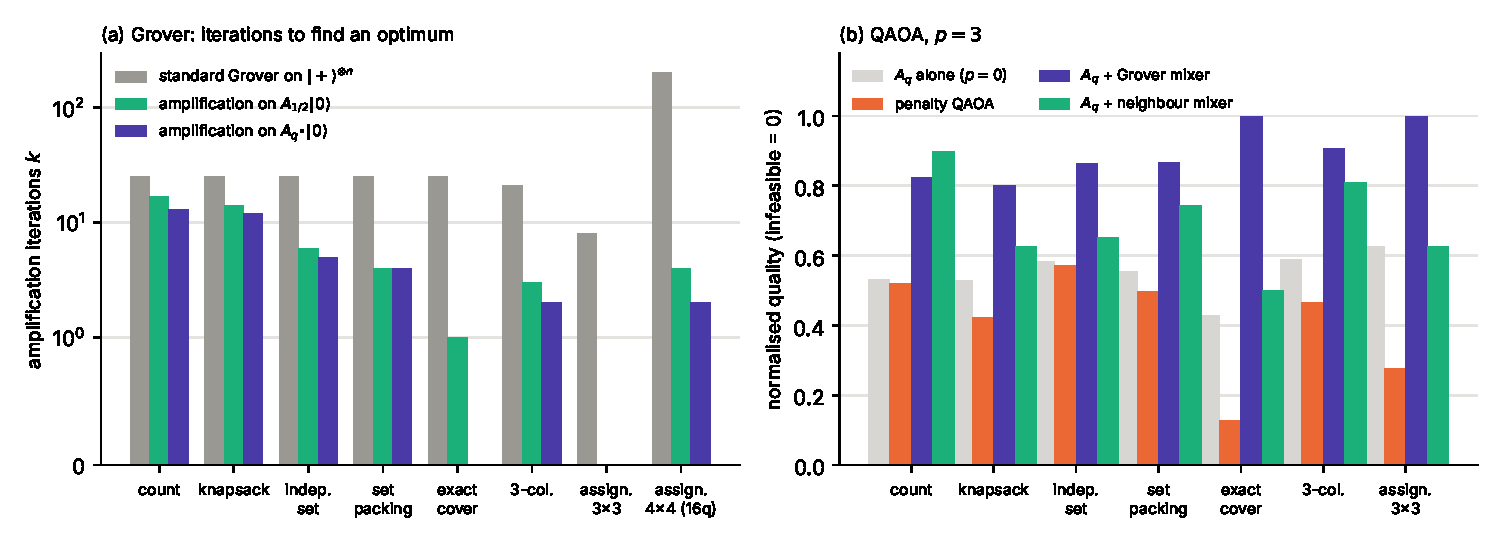
\includegraphics[width=\textwidth]{figures/fig_general.pdf}
\caption{\orig{exact ideal numerics} One pipeline on seven constraint types. (a) Amplification iterations to find an optimum: standard Grover, $A_{1/2}$, and $A_q$ with the best bias (symmetric log axis); a missing bar is $k=0$, i.e.\ measuring $A_q|0\rangle$ already finds an optimum with high probability. (b) QAOA at $p=3$: quality, infeasible samples counted as $0$.}\label{fig:general}
\end{figure*}

\paragraph{Amplification.} The gain follows the tightness of the constraint. With loose constraints (cardinality, knapsack; $|F|/2^n\approx0.2$--$0.4$) the saving is $1.5$--$2\times$ ($25\to17$ and $25\to14$ iterations at $q=\tfrac12$). With tight constraints it is large: independent set $25\to6$, set packing $25\to4$, $3$-colouring $21\to3$, exact cover $25\to1$; for $3\times3$ assignments the optimum is found by measuring $A_q|0\rangle$, and for $4\times4$ permutations ($24$ feasible strings among $65\,536$) standard Grover needs $201$ iterations and $A_q$ needs $4$ ($2$ with the best bias).

\paragraph{QAOA.} With the Grover mixer every sample is feasible, at every depth and for arbitrary angles (the smallest feasible mass over all instances, depths and methods is $1-3\cdot10^{-16}$). Penalty QAOA, with the best of four penalty weights, has $21$--$95\,\%$ feasible samples, falling with the tightness, and a lower quality on all seven families; at $p=3$ the Grover mixer wins in quality on $34$ of $34$ instances (median $0.80$--$1.00$ against $0.13$--$0.57$). For the $4\times4$ assignment penalty QAOA gives $2.6\,\%$ feasible samples and quality $0.014$, against $100\,\%$ and $0.82$ for $A_q$. Two caveats: exact cover and assignment have only $3$--$6$ feasible strings, so they show the mechanism and not difficulty; and local mixers need a connected move graph (the neighbour mixer does not move the state on exact cover and permutations), so cheap mixers are structure-dependent while the Grover mixer is general at the price of two copies of $A_q$ per layer.

\paragraph{Circuits and scale.} The compiled circuits reproduce the exact formulas to $8\cdot10^{-15}$ (all Grover iterations) and $5\cdot10^{-16}$ ($p=2$ QAOA); the compiled $A_q$ costs $24$--$297$ CZ gates for the six $n=6$ families, without hand optimisation. With the automaton written from the structure of the problem, the same compiler runs on matrix-product states up to $60$ variables for a cardinality constraint ($274$ qubits), $80$ for a band independent set ($236$) and $30$ for knapsack ($145$); all $15$ instances ($7$ configurations) give $100\,\%$ feasible shots against uniform feasible shares down to $2\cdot10^{-11}$. These runs validate the circuits at scale and say nothing about advantage.

\paragraph{Where it fails.} Market split ($m$ equalities on random integers) is the opposite case: exact look-ahead would solve the instance, and the practical bound-only relaxation has width $21$ at $n=10$ and $12\,067$ at $n=20$, while the iterations shrink only fourfold. There the circuit grows faster than the iterations shrink and the construction does not pay. The width--completeness dial is monotone and sound: tracking a knapsack weight only up to a lower bound reduces the width from $33$ to $1$, and the iterations rise from $25$ to the $50$ of standard Grover (\cref{prop:relax}).

\section{From theory to circuits: classical reduction and the residual quantum core}\label{sec:reduction}
Feasibility by construction is only useful if the circuit can be run. We test this on a multi-period long/short portfolio with sector caps, long/short exclusivity, a per-period capital and budget, and a global trading budget: $A=12$ assets in three sectors and $T=8$ periods give $n=192$ variables and $137$ constraints of four kinds, with a quadratic risk objective (\cref{sec:large}).

\paragraph{The coherent state does not fit.} The automaton over all constraints has width $11$ at $n=24$ and $103$ at $n=192$, because the global budget couples all periods, and the compiled $A_q$ grows from $12.9$ thousand CZ gates and $88$ qubits to $5.1$ million and $1156$ qubits (default synthesis, before routing). The feasible share of the uniform state is $2^{-131}$, which is what the construction repairs, but the circuit is far beyond any device.

\paragraph{Reduction derived from the automaton.} Three classical steps act before any circuit is built. (i)~\emph{Variable order}: period-major gives widths $8$, $23$, $11$ against $36$, $172$, $36$ for asset-major on three small instances. (ii)~\emph{Conditioning on an interface}: drawing the per-period and per-sector counts of longs and shorts classically makes the periods independent blocks and the cost linear in $T$, from $5.1$ million to $29$ thousand CZ gates at $n=192$, and to about $2.9$ thousand with a second level of conditioning and one-hot registers. (iii)~\emph{Symmetry-aware lowering}: in each block the (long, short) pairs of the assets are interchangeable (an automatic check on $F$), so the block is prepared with Dicke states and a chain of controlled swaps, exactly uniform on the feasible set, with no register and no uncomputation; per block it is $3.1$--$4.4\times$ smaller than the generic circuit and $5$--$8\times$ when the generic registers must be uncomputed, as QAOA with pair-exchange mixers requires (for the preparation of a whole core the ratio is $14$--$28\times$, \cref{sec:sota}). This lowering is not specific to our construction (Dicke states are known); the role of the automaton there is to detect the structure and guarantee the support.

\paragraph{What conditioning costs.} The interface is drawn classically, so the superposition over interface values becomes a mixture. That is valid for sampling and for QAOA with mixers that conserve the interface (case (b) of \cref{thm:qaoa}), and invalid for amplification of the whole state and for the global Grover mixer, which need coherence across interface values.

\paragraph{Exact pruning, and how much is left.} Given the interface, variables that take the same value in all feasible strings of their block are known: they leave the objective, blocks with a single feasible string need no mixer, blocks without longs or shorts use a two-qubit swap rotation instead of a four-qubit pair exchange, and a constraint gauge rewrites couplings with the constant counts. The state on the feasible set is unchanged (checked against dense simulation to $10^{-14}$) and the compiled layer shrinks $4$--$8\times$ (at $n=24$, $1131\to259$--$262$ CZ, median ESP $0.01\to0.36$--$0.38$; \cref{tab:core_prune}). The reduction is large because the interface fixes most variables: on average only $2.5$, $6.0$, $6.9$ and $11.1$ of $8$, $12$, $16$ and $24$ variables stay free. This must qualify every size quoted for executability: what is left to the quantum computer is a \emph{core}, and its size, not that of the original problem, is what a device must run.

\begin{table}[t]
\centering\footnotesize\setlength{\tabcolsep}{4pt}
\caption{\orig{exact classical counting and sampling; no circuits} Residual quantum core after the exact classical reduction, over $200$ sampled interface tuples per row. Families differ in how loose the local constraints are (tight: at most one long position per sector and $3$ positions per period; medium: $2$, $6$; loose: $4$, $12$). Free: qubits that remain (upper bound); $\log_2|F|$: feasible strings of the core; ZZ: couplings among free variables for a dense objective.}\label{tab:core_map}
\begin{tabular}{lrrrr}
\toprule
family & $n$ & free & $\log_2|F|$ & ZZ\\
\midrule
tight & 96 & 42 & 18 & 881\\
tight & 192 & 84 & 25 & 3528\\
tight & 384 & 168 & 50 & 14112\\
tight & 768 & 336 & 64 & 56448\\
medium & 96 & 58 & 28 & 1691\\
medium & 192 & 113 & 44 & 6432\\
medium & 384 & 221 & 89 & 24605\\
medium & 768 & 437 & 120 & 95816\\
loose & 96 & 84 & 41 & 3535\\
loose & 192 & 137 & 71 & 9497\\
loose & 384 & 254 & 138 & 32406\\
loose & 768 & 478 & 203 & 114381\\
\bottomrule
\end{tabular}
\end{table}


\paragraph{How large can the core be?} The average above is for $n\le24$. \Cref{tab:core_map} counts the core for families of different looseness and up to $768$ variables: the share of free variables is $44$--$46\,\%$ for tight constraints and $62$--$88\,\%$ for loose ones, so the core grows with the problem, to $42$--$84$ free qubits for tight constraints at $n=96$--$192$ and to hundreds for loose ones. With tight constraints the core is still enumerable up to about $n=192$ ($2^{25}$ feasible strings) and needs no quantum treatment there; with loose constraints it has $2^{41}$ feasible strings at $n=96$ and $2^{138}$ at $n=384$, so enumeration is impossible and a quantum treatment of the core could matter. Such cores are far beyond what a device is predicted to run (\cref{sec:sota}). The reduction is preprocessing that benefits any quantum method equally; the size of the core is a property of how loose the constraints are.

\section{Comparison with quantum baselines, and what hardware could run}\label{sec:sota}
The question here is not whether a quantum circuit beats a classical solver; it is how our layer compares with other \emph{quantum} treatments of the same constraints, and what a device could run. On the same residual core, with the same classically reduced objective, we compare our QAOA layer with unbalanced penalisation~\cite{montanez2024unbalanced}, with the single-basis-circuit form of Fourier-based LCU~\cite{carrera2026fourier} (one trained $R_z$ angle per count constraint and a trained single-qubit mixer; not its sampling machinery) and with QAOA with an XY mixer inside every count group, the coherent circuit that the LCU approximates. Plain penalty QAOA was the weaker baseline in \cref{sec:validation} and \cref{sec:large} and is not repeated here.

\paragraph{Gate counts.} Unbalanced penalisation and the LCU form add no two-qubit gates beyond the objective: the constraint layer is single-qubit or falls on pairs the dense objective already couples. Our layer adds the preparation and the mixers, $77\,\%$ to $14\,\%$ of the objective's gates as the core grows from $48$ to $512$ variables (before routing). After routing to heavy-hex our layer has $1.9$--$2.5\times$ the CZ gates and $2.6$--$3.7\times$ the depth of a uniform-start baseline on average over six cores of $16$--$64$ qubits; on the cores below it has $1.2$--$1.9\times$ the CZ gates of the warm-started LCU and unbalanced circuits and $0.95$--$1.4\times$ those of the XY circuit. Per layer it is therefore somewhat more expensive; what it buys is that every sample is feasible.

\paragraph{Baselines, weak and strong.} In a first comparison (\cref{tab:core_cases}) Fourier-LCU and unbalanced start from the uniform state, as in common QAOA implementations. This is a weak baseline: the Fourier-LCU paper warm-starts every qubit with $R_Y(2\arcsin\sqrt{k/n})$, a product state whose probability of satisfying a cardinality constraint is $\Theta(1/\sqrt n)$. \Cref{tab:core_baselines} gives all baselines this start and trains them with $12$ restarts ($4$ at $20$ qubits) in dense simulation; the compiled circuits equal the simulation to $10^{-15}$. Everything is on cores that were chosen to fit ($16$ and $20$ free qubits; a typical interface leaves tens of free qubits, $42$--$84$ for tight constraints at $n=96$--$192$, \cref{tab:core_map}, which no method is predicted to run).

\begin{table*}[t]
\centering\footnotesize\setlength{\tabcolsep}{4pt}
\caption{\orig{compiled counts; ideal feasibility and quality from exact simulation; success probabilities from the ESP model; nothing executed} Three cases, one $p=1$ layer on the residual core, compiled to \texttt{ibm\_fez} (best of $3$--$4$ seeds). Feasible, quality ($1$ is the optimum, among feasible samples) and $P(\mathrm{opt})$ are ideal-simulation values; the Fourier-LCU and unbalanced baselines here start from the uniform state (a weak baseline; warm-started ones in \cref{tab:core_baselines}), were trained in dense simulation with few restarts, and at $n=192$ are compiled only. The cores were chosen to fit ($16$, $20$, $30$ free qubits). Grover rows: one compiled iteration with an ancilla-free and a V-chain reflection, and the iterations needed; $|F|$: feasible strings of the core.}\label{tab:core_cases}
\begin{tabular}{rrrlrrrrrr}
\toprule
$n$ & free & $|F|$ & method & CZ & depth & ESP & feas. & qual. & $P$(opt)\\
\midrule
64 & 16 & 64 & ours (QAOA) & 473 & 541 & 0.191 & 100\,\% & 0.67 & 4.18\,\%\\
 & &  & Fourier-LCU & 412 & 525 & 0.235 & 17\,\% & 0.73 & 0.96\,\%\\
 & &  & unbalanced & 412 & 525 & 0.234 & 11\,\% & 0.65 & 0.62\,\%\\
 & & & ours (Grover, 1 it., no ancilla) & 3454 & 8025 & $5.3\cdot10^{-6}$ & \multicolumn{3}{l}{16 qubits; 6 iterations}\\
 & & & ours (Grover, 1 it., V-chain) & 323 & 578 & 0.306 & \multicolumn{3}{l}{31 qubits; 6 iterations}\\
\midrule
100 & 20 & 5000 & ours (QAOA) & 669 & 607 & 0.066 & 100\,\% & 0.65 & 0.40\,\%\\
 & &  & Fourier-LCU & 413 & 307 & 0.184 & 10\,\% & 0.65 & 0.03\,\%\\
 & &  & unbalanced & 413 & 310 & 0.184 & 12\,\% & 0.52 & 0.0086\,\%\\
 & & & ours (Grover, 1 it., no ancilla) & 6270 & 14390 & $5.1\cdot10^{-11}$ & \multicolumn{3}{l}{20 qubits; 56 iterations}\\
 & & & ours (Grover, 1 it., V-chain) & 800 & 968 & 0.033 & \multicolumn{3}{l}{40 qubits; 56 iterations}\\
\midrule
192 & 30 & 303750 & ours (QAOA) & 923 & 586 & 0.037 & 100\,\% & 0.59 & 0.0021\,\%\\
 & &  & Fourier-LCU & 612 & 414 & 0.120 & -- & -- & --\\
 & &  & unbalanced & 614 & 418 & 0.119 & -- & -- & --\\
 & & & ours (Grover, 1 it., no ancilla) & 8743 & 19188 & $2.7\cdot10^{-20}$ & \multicolumn{3}{l}{30 qubits; 433 iterations}\\
 & & & ours (Grover, 1 it., V-chain) & 1279 & 1555 & $3.2\cdot10^{-3}$ & \multicolumn{3}{l}{64 qubits; 433 iterations}\\
\bottomrule
\end{tabular}
\end{table*}


\begin{table*}[t]\centering\scriptsize\setlength{\tabcolsep}{3pt}
\caption{\orig{compiled counts; ideal feasibility, quality and $P(\mathrm{opt})$ from exact dense simulation; per-shot values from the ESP and depolarising model; nothing executed} Stronger baselines on the residual core: ws = warm start: all baselines start from the warm-started product state of the Fourier-LCU paper (RY$(2\arcsin\sqrt{k/m})$ per qubit) and are trained with $12$ restarts ($p=1$). Mean $\pm$ standard deviation over instances (objective seeds $\times$ interface tuples). Feasible, quality (among feasible samples) and $P(\mathrm{opt})$: ideal. Last column: probability of the optimum per shot under the depolarising model with the ESP of the compiled circuit.}\label{tab:core_baselines}
\begin{tabular}{llrrrrrr}\toprule
core & method & CZ & ESP & feas. & quality & $P$(opt) ideal & $P$(opt) per shot (model)\\\midrule
$n=64$, $f=16$ (6 inst.) & ours ($F$) & $352\pm100$ & $0.320\pm0.117$ & $100\pm0$\,\% & $0.71\pm0.03$ & $3.68\pm0.90$\,\% & $1.272\pm0.708$\,\%\\
 & Fourier-LCU, ws & $277\pm94$ & $0.416\pm0.138$ & $18\pm4$\,\% & $0.72\pm0.11$ & $1.37\pm0.67$\,\% & $0.585\pm0.429$\,\%\\
 & unbalanced, ws & $277\pm94$ & $0.417\pm0.139$ & $70\pm0$\,\% & $0.54\pm0.05$ & $1.15\pm0.00$\,\% & $0.481\pm0.160$\,\%\\
 & XY mixer, ws & $363\pm111$ & $0.319\pm0.124$ & $15\pm0$\,\% & $0.70\pm0.03$ & $0.63\pm0.22$\,\% & $0.217\pm0.131$\,\%\\
\midrule
$n=100$, $f=20$ (4 inst.) & ours ($F$) & $555\pm0$ & $0.162\pm0.000$ & $100\pm0$\,\% & $0.75\pm0.06$ & $0.46\pm0.40$\,\% & $0.075\pm0.065$\,\%\\
 & Fourier-LCU, ws & $299\pm0$ & $0.368\pm0.000$ & $3\pm1$\,\% & $0.72\pm0.05$ & $0.12\pm0.20$\,\% & $0.044\pm0.075$\,\%\\
 & unbalanced, ws & $296\pm3$ & $0.373\pm0.004$ & $44\pm0$\,\% & $0.57\pm0.07$ & $0.00\pm0.00$\,\% & $0.002\pm0.000$\,\%\\
 & XY mixer, ws & $391\pm0$ & $0.272\pm0.001$ & $1\pm0$\,\% & $0.76\pm0.06$ & $0.01\pm0.01$\,\% & $0.003\pm0.003$\,\%\\
\bottomrule
\end{tabular}\end{table*}


\paragraph{Results.} With the uniform start the baselines give $10$--$17\,\%$ feasible samples at $16$ and $20$ qubits, and our layer's probability of the optimum per shot under the noise model is $3.5$--$16\times$ theirs (\cref{tab:core_cases}). The warm start closes much of that gap (\cref{tab:core_baselines}). In ideal simulation at $p=1$, on the $16$-qubit core (six instances), our layer gives $100\,\%$ feasible samples, quality $0.71$ among feasible samples and $P(\mathrm{opt})=3.7\,\%$; the warm-started LCU gives $18\,\%$, $0.72$ and $1.4\,\%$, unbalanced penalisation $70\,\%$ (and $96\,\%$ at $p=2$), $0.54$ and $1.2\,\%$, and the XY mixer $15\,\%$, $0.70$ and $0.6\,\%$. At $p=2$ our layer reaches $P(\mathrm{opt})=8.3\,\%$ against $6.5\,\%$ for the LCU, whose quality ($0.82$) is above ours ($0.77$) but whose results vary by an order of magnitude between instances. At $20$ qubits (four instances, with four restarts in two and eight in the other two) the baselines are weaker, with $2$--$6\,\%$ (LCU), $44\,\%$ (unbalanced) and $1\,\%$ (XY) feasible samples. Under the depolarising model, with the ESP of each compiled circuit (our layer has more CZ gates than the warm-started LCU and unbalanced circuits), the probability of the optimum per shot is $1.3\,\%$ for our layer against $0.59\,\%$, $0.48\,\%$ and $0.22\,\%$ at $16$ qubits, between $1.2$ and $3.3$ times that of the best baseline in each of the six instances. At $20$ qubits the per-shot probability of the optimum is small for every circuit ($0.01$--$0.18\,\%$ for ours) and varies by an order of magnitude between instances: our layer is the best in three of the four instances (by $7$, $22$ and $22$ times over the best baseline) and $2.5$ times worse in one, where the single-basis LCU reaches $0.17\,\%$ against our $0.07\,\%$; with this model the unbalanced circuit stays at $0.002\,\%$ because its feasible fraction is lowered by the noise. Across all ten instances our layer is best in nine, which is a small sample. The honest summary is that the feasible-by-construction layer keeps its structural advantage ($100\,\%$ feasible samples, no penalty weights to tune) and an advantage per shot that is modest at $16$ qubits and larger but erratic at $20$, and that it depends on how well the baselines are trained.

\paragraph{Noise model.} We use three levels, in increasing cost: ESP (the product of one minus the error of every compiled gate), a global depolarising model ($\mathrm{ESP}\cdot P_\mathrm{ideal}+(1-\mathrm{ESP})\cdot\mathrm{uniform}$) and, up to about $20$ qubits, a gate-level Aer simulation with the FakeFez noise model. On one $16$-qubit core the model is only slightly conservative ($18.1\,\%$ feasible shots against $21.8\pm1.7\,\%$ simulated for our layer, $600$ shots; \cref{sec:core}). Per-shot values in this section are predictions, not measurements, and apply to the models of two small cores.

\begin{table*}[t]
\centering\footnotesize\setlength{\tabcolsep}{4pt}
\caption{\orig{estimate, an extrapolation of the ESP model; no hardware} What one QAOA layer needs. Effective error per CZ $\varepsilon=-\ln(\mathrm{ESP})/\#\mathrm{CZ}$ over nine compiled circuits (median $0.0035$). ESP of our layer at $473$, $669$, $923$ CZ if the error per CZ were reduced by the factor shown; last columns: free qubits whose layer keeps ESP $\ge0.3$ and $\ge0.1$ at $\approx31$ CZ per free qubit (a dense objective gives fewer). The scaling of the error rate is an assumption.}\label{tab:core_hw}
\begin{tabular}{lrrrrr}
\toprule
error per CZ & ESP$_{16}$ & ESP$_{20}$ & ESP$_{30}$ & free qubits, ESP$\ge0.3$ & ESP$\ge0.1$\\
\midrule
today ($\varepsilon\approx0.0035$) & 0.19 & 0.09 & 0.04 & 11 & 21\\
$3\times$ better & 0.57 & 0.46 & 0.34 & 33 & 63\\
$10\times$ better & 0.85 & 0.79 & 0.72 & 110 & 211\\
\bottomrule
\end{tabular}
\end{table*}


\paragraph{Does the block grow with the number of constraints?} \orig{exact enumeration and compiled counts to $\{$CX, Rz, SX, X$\}$, all-to-all; no noise, no device} It depends on whether the constraints decompose (\path{experiments/constraint_scaling*.py}; the three parts below are the three panels of \cref{fig:constraint_scaling}). (a)~\emph{Panel (a).} For disjoint cardinality constraints the block is one Dicke state per group and the depth is that of the largest group: at $n=24$, going from $m=1$ to $12$ groups lowers it from $1761$ to $13$, and adding groups of the same size leaves it unchanged while the CZ count grows linearly. A penalty layer is cheaper per constraint ($552$ CZ and depth $135$ against $1962$ and $1761$ for one group of $24$, or $981$ CZ with the optimised Dicke block of \cref{sec:core}) but does not give feasible samples. (b)~\emph{Panel (b).} For overlapping constraints the generic automaton circuit does grow: with random constraints (five of $14$ variables, at most two) the width goes from $3$ to about $40$ and the circuit from $293$ to $1.7\cdot10^{4}$ CZ for eight constraints, while a penalty layer grows from $20$ to $116$ CZ. In that regime the construction is not competitive in gate count. (c)~\emph{Panel (c).} Interface conditioning is what restores a small block: fixing the $s$ most frequent variables classically halves the width for each variable fixed (mean CZ per branch over two instances: $1.7\cdot10^4$ at $s=0$, $1.6\cdot10^3$ at $s=3$ and $1.6\cdot10^2$ at $s=6$), at the price of $7$ and about $33$ classical branches. So the block is constant in the number of constraints only for the part that decomposes; the rest is moved to the classical interface, whose size is the real cost of the method.

\paragraph{What a device could run.} The effective error per CZ over all nine compiled circuits is $0.0035$--$0.0041$, which gives $\mathrm{ESP}\approx e^{-0.0035\,N_\mathrm{CZ}}$, and one free qubit costs about $31$ CZ in these cores (the objective couples only variables of one period). A layer with ESP $\ge0.3$ then allows about $11$ free qubits and one with ESP $\ge0.1$ about $21$ (\cref{tab:core_hw}); our layer compiles to $473$, $669$ and $923$ CZ for $16$, $20$ and $30$ free qubits, with ESP $0.19$, $0.066$ and $0.037$. Post-selection on feasibility is free for a feasible-by-construction circuit and turns noise into a loss of shots by $1/\mathrm{ESP}$ rather than a distortion: on the $16$-qubit core the quality after post-selection is $0.713$ against $0.717$ ideal. It does not catch errors that map a feasible string to another feasible string. Error cancellation would cost about $e^{4\varepsilon N_\mathrm{CZ}}$ ($7\cdot10^2$ at $473$ CZ, $4\cdot10^5$ at $923$) and is not used; dynamical decoupling, twirling and readout mitigation were not applied in the estimates.

\paragraph{The generic automaton does not run at these sizes.} With the generic automaton preparation the layer takes $2.0$, $2.9$ and $4.9$ thousand CZ gates against $464$, $581$ and $923$ for the symmetric lowering, even with measurement-based uncomputation (\cref{sec:core}). \emph{So the part specific to us, the automaton for arbitrary constraints, is not predicted to run on today's devices at these sizes; what is predicted to run is its symmetric special case.}

\paragraph{Amplitude amplification is a fault-tolerant use.} Among the QAOA variants compared here only ours admits it. One iteration costs $3.5$, $6.3$ and $8.7$ thousand CZ with an ancilla-free reflection, and $323$, $800$ and $1279$ with a Toffoli V-chain ($10.7\times$ to $6.8\times$ fewer; $31$, $40$ and $64$ qubits), with ESP per iteration $0.31$, $0.033$ and $0.003$ against the $6$, $56$ and $433$ iterations needed. Its advantage appears for large cores, where it needs $2^{4}$--$2^{6}$ times fewer iterations than Grover over all strings in the cases above and up to $2^{95}$ in the larger cores of \cref{sec:core} ($23$--$326$ free qubits); a fault-tolerant cost model ($88$--$1156$ logical qubits) is in \cref{sec:large}.

\paragraph{Combining with other methods.} A diagonal layer of any kind keeps the support, so \emph{any approximation of the objective layer preserves feasibility} and only affects quality. (This paragraph uses a second interface tuple per size, \cref{sec:core}, so its values are comparable only within it.) Without the two-qubit objective layer, our preparation and mixers compile to $66$, $260$ and $357$ CZ gates with ESP $0.80$, $0.41$ and $0.24$, against $0.20$, $0.15$ and $0.04$ with it. Replacing the objective by a single-qubit mean-field layer, as the cheapest stand-in for a Fourier-type decomposition, keeps the quality in ideal simulation ($0.741$, $0.700$, $0.622$ against $0.731$, $0.677$, $0.599$ with the full layer). The stand-in is not the LCU method, and the mean-field problem is trivial classically, so a quantum layer on top of it adds value only if it improves on the classical solution of that linearisation, which was not tested.

\paragraph{A 120-qubit experiment, specified and not run.} The estimates above concern one core at a time. To use a chip of more than $100$ qubits, we use the independence the interface gives: a portfolio with $n=120$ variables splits into twelve blocks of $10$ qubits, each with its own quadratic objective, placed on disjoint regions of $11$ physical qubits (a chip with at least $132$ usable qubits, such as the $156$-qubit \texttt{ibm\_fez}) and run as one circuit of $120$ measured qubits. Twelve circuits are specified (ours light and full, ours preparation only, a Hadamard control, the warm-started Fourier-LCU variant, unbalanced penalty and XY-mixer QAOA, trained and given the same decomposition, which is the setting most favourable to them, and, for the cost-informed preparation of \cref{sec:core}, our tilted preparation alone and with $p=1$ against the three baselines given the same classical information), together with five criteria fixed before any run (\cref{app:hw100}). \Cref{tab:hw100_pred} gives the compiled counts and the noise-model prediction: the preparation alone is predicted to give about $67\,\%$ feasible shots per block against $28\,\%$ for the warm-started unbalanced circuit, $11$--$12\,\%$ for the LCU and XY circuits and $1.7\,\%$ for the control; our $p=1$ layer gives $22\,\%$ (light) and $13\,\%$ (full), below the unbalanced circuit, because the layer costs three to four times the preparation; and the LCU and XY circuits are predicted to have a better quality among their feasible samples ($0.71$ and $0.70$ against $0.66$). So the clearest prediction is for the preparation alone, not for the $p=1$ layer. With the classical tilt (same gates, other Dicke angles) the preparation alone is predicted to give $66\,\%$ feasible shots per block and a quality of $0.79$, against $14$--$33\,\%$ and $0.83$--$0.88$ for the baselines that receive the same information: the tilt raises every circuit's quality, and ours keeps the lead in feasibility, not in quality. Blocks of ten qubits are classically trivial, so the experiment would show feasibility at a scale where global-constraint methods have no chance, not an advantage. The experiment is released as notebooks and has not been run.

\begin{table*}[t]\centering\small
\caption{\orig{compiled counts; ideal values from exact simulation; noisy values from the depolarising model; nothing executed} Predictions for the 120-qubit experiment (twelve blocks of $10$ qubits in one circuit; averages over blocks; CZ and ESP: median per block, depth: maximum). Feasible: share of shots of a block that satisfy its constraints; quality: $1-$normalised cost among feasible shots (uniform on the feasible set: about $0.5$). Not measured.}\label{tab:hw100_pred}
\begin{tabular}{lrrrrrrr}\toprule
method & CZ & depth & ESP & feas. ideal & feas. model & qual. ideal & qual. model\\\midrule
ours, $p{=}1$ light & 338 & 1008 & 0.22 & 1.000 & 0.220 & 0.67 & 0.66\\
ours, $p{=}1$ full & 447 & 1196 & 0.11 & 1.000 & 0.134 & 0.72 & 0.69\\
ours, preparation only & 96 & 449 & 0.71 & 1.000 & 0.669 & 0.50 & 0.50\\
uniform (Hadamards) & 0 & 4 & 1.00 & 0.017 & 0.017 & 0.50 & 0.50\\
Fourier-LCU, warm start & 154 & 296 & 0.47 & 0.244 & 0.122 & 0.74 & 0.71\\
unbalanced, warm start & 154 & 299 & 0.47 & 0.589 & 0.281 & 0.51 & 0.51\\
XY mixer, warm start & 194 & 342 & 0.41 & 0.239 & 0.107 & 0.73 & 0.70\\
ours, tilted preparation only & 99 & 457 & 0.69 & 1.000 & 0.660 & 0.80 & 0.79\\
ours, tilted, $p{=}1$ light & 342 & 1028 & 0.21 & 1.000 & 0.217 & 0.85 & 0.82\\
Fourier-LCU, tilted start & 154 & 298 & 0.47 & 0.375 & 0.182 & 0.91 & 0.88\\
unbalanced, tilted start & 153 & 296 & 0.47 & 0.690 & 0.330 & 0.84 & 0.83\\
XY mixer, tilted start & 192 & 344 & 0.40 & 0.326 & 0.138 & 0.91 & 0.87\\
\bottomrule\end{tabular}\end{table*}


\paragraph{Depth and cost on IBM hardware at 120 qubits.} \orig{compiled counts and an estimate; nothing executed} \Cref{tab:hw100_cost} adds the total depth and the two-qubit depth of the same circuits. The twelve blocks run in parallel, so depth does not grow with the number of blocks: our $p=1$ light layer has depth $1008$ and two-qubit depth $310$ ($4128$ CZ in all, about $344$ per block), the full layer $1196$ and $371$, the preparation alone $449$ and $149$, and the baselines $296$--$342$ and $103$--$115$ ($1838$ CZ for the LCU and unbalanced circuits, $2289$ for the XY mixer). Our layer therefore has about three times the two-qubit depth of the LCU and unbalanced circuits, and the preparation alone about $1.4\times$ with $34\%$ fewer CZ gates; the tilt changes these numbers by less than $4\%$. The scheduled duration is $13$--$44\,\mu$s per shot, so the time on the device is set by the repetition delay (default $250\,\mu$s) and the readout, not by the circuit: about $2.6$--$2.9$ s per $10^4$ shots for each circuit, $\approx11$ s for the four-circuit comparison (ours with and without the layer, LCU, unbalanced) and $\approx32$ s for all twelve. At the pay-as-you-go price listed by IBM ($\$96$ per minute of QPU time, billed per second) this is about $\$4.3$ per circuit, $\$17$ for the four-circuit comparison and $\$51$ for all twelve per $10^4$ shots, before the job overhead, which we did not estimate; a $10^5$-shot run multiplies it by ten. Whether a $156$-qubit device is available in the free plan ($10$ minutes per $28$ days) depends on the account. These are estimates from a calibration snapshot, not measurements; the total and two-qubit depths of the $16$--$30$-qubit cores of \cref{sec:core} were not recompiled.
\begin{table}[t]\centering\scriptsize\setlength{\tabcolsep}{2pt}
\caption{\orig{compiled counts on the \texttt{ibm\_fez} snapshot; time is an estimate; nothing executed} The $120$-qubit circuits (twelve blocks in one circuit): total depth, two-qubit depth, CZ gates (all blocks), scheduled duration and estimated QPU time for $10^4$ shots (duration plus the default repetition delay of $250\,\mu$s per shot; job overhead not included).}\label{tab:hw100_cost}
\begin{tabular}{lrrrrr}\toprule
circuit & depth & 2q depth & CZ & dur. ($\mu$s) & QPU s\\\midrule
ours $p{=}1$ light & 1008 & 310 & 4128 & 37 & 2.9\\
ours $p{=}1$ full & 1196 & 371 & 5466 & 44 & 2.9\\
ours, preparation & 449 & 149 & 1220 & 18 & 2.7\\
uniform & 4 & 0 & 0 & 2 & 2.5\\
Fourier-LCU, ws & 296 & 103 & 1838 & 13 & 2.6\\
unbalanced, ws & 299 & 103 & 1838 & 13 & 2.6\\
XY mixer, ws & 342 & 115 & 2289 & 15 & 2.6\\
ours tilted, prep. & 457 & 143 & 1230 & 18 & 2.7\\
ours tilted $p{=}1$ & 1028 & 319 & 4164 & 38 & 2.9\\
LCU, tilted start & 298 & 103 & 1838 & 13 & 2.6\\
unbalanced, tilted start & 296 & 103 & 1797 & 13 & 2.6\\
XY, tilted start & 344 & 115 & 2274 & 15 & 2.6\\
\midrule
all twelve circuits & & & & & 32\\
\bottomrule\end{tabular}\end{table}



\section{Discussion and limitations}\label{sec:discussion}
\paragraph{What is established.} The theory holds in every case checked: feasibility by construction, amplification and QAOA invariance, and the compiled circuits equal the ideal simulation to $10^{-14}$. The classical reduction derived from the automaton is exact and large, and it benefits any quantum method equally; it leaves a core that is small in absolute terms only at about $24$ variables or fewer (a few free qubits on average) and that grows to tens or hundreds of qubits at $96$--$768$ variables. Compiled for the \texttt{ibm\_fez} topology, our layer on cores of $16$--$20$ free qubits has an estimated success probability of $0.07$--$0.19$ (noise model); it gives $100\,\%$ feasible samples and quality above uniform sampling of the feasible set in ideal simulation. It costs $1.2$--$1.9$ times the CZ gates of the warm-started LCU and unbalanced circuits. Under the noise model it is predicted to give $1.2$--$3.3$ times the probability of the optimum per shot of the best warm-started baseline at $16$ free qubits (six instances), and an erratic result at $20$ (four instances); against uniform-start baselines the factor is $3.5$--$16$. Its quality among feasible samples is equal to that of the LCU at $p=1$ and below it at $p=2$ ($0.77$ against $0.82$), and the LCU's results vary widely between instances. The advantage that remains beyond that is amplification, in the fault-tolerant regime.
\paragraph{What is not.} We make no claim relative to classical solvers, which is not the question asked here. The comparison with the quantum baselines is limited to cores of $16$ and $20$ qubits (six and four instances), with $12$ restarts at $16$ qubits and $4$ to $8$ at $20$, a Fourier-LCU in its single-basis-circuit form that omits the sampling machinery and the CVaR objective of the original, and interface tuples chosen so that the core fits; the cores at $16$ qubits are small ($|F|=64$, two count groups); at larger sizes the baselines were only compiled. The generic automaton, the part specific to this construction, is not predicted to run at the sizes above even with measurement-based uncomputation; what is predicted to run is its symmetric special case, which is not specific to us. Conditioning on an interface turns the global superposition into a statistical mixture of branches: it is compatible with QAOA with independent block mixers, but it gives up the coherence that global amplification and the global Grover mixer need, so the amplification advantage is not available in the regime in which the hardware figures were obtained. The hardware figures are compiled counts, noise-model predictions and gate-level simulations, whose gap to a device (crosstalk, drift, non-depolarising noise) is unknown: the $120$-qubit experiment that would close it is released but not run, and it may fail its own criteria (the objective layer may not pay off at these depths). The numerics are small (the truth-table automaton limits $n\le16$; larger runs use automata written from the structure), QAOA angles are local optima, and exact cover and assignment have tiny feasible sets.
\paragraph{Outlook.} Four directions follow: informed preparation, where constraint propagation and local consistency are compiled into the coherent state and whose benefit can be computed exactly beforehand; compilation that optimises jointly over logic, non-Clifford cost and routing, including a lowering of counting automata that would remove Toffoli gates (untested); richer constraint languages (pseudo-Boolean and mixed-integer constraints, routing, verification); and hybridisation with classical reasoning engines, with the quantum routine as an amplification module receiving the propagation rules a classical solver has already derived. The immediate steps are the run of the $120$-qubit experiment and its repetition with the original Fourier-LCU as baseline.

\section{Conclusion}
A constraint automaton turns every constraint set into a state preparation whose support is exactly the feasible set. Over it, amplitude amplification needs at most Grover's iterations with an objective-only oracle, and QAOA with the Grover mixer or any feasibility-preserving mixer is feasible at every depth and for all angles. One compiler reproduces the exact formulas at gate level on seven constraint types and fails where the theory says it should. On a $192$-variable portfolio, classical reduction from the automaton leaves a core of a few free qubits at $24$ variables and of tens to hundreds at $96$--$768$; on cores of $16$--$20$ free qubits our layer is feasible at every shot in ideal simulation, costs $1.2$--$1.9$ times the CZ gates of the warm-started quantum baselines, and is predicted by a noise model (which agrees within about $20\,\%$, conservatively, with a gate-level simulation on one $16$-qubit core) to give $1.2$--$3.3$ times the best baseline's probability of the optimum per shot at $16$ free qubits, a margin that is not robust at $20$. The two halves of the result must be read together. Compatibility with Grover's algorithm depends on keeping the full coherent superposition over the feasible set, and for the general automaton the number of gates needed for that superposition grows with the width, which is exponential in the worst case; sampling the interface classically avoids that cost by replacing the global superposition with a statistical mixture of branches, which suits QAOA with independent block mixers and which \emph{removes} global amplitude amplification. Amplification is therefore a fault-tolerant use, and the near-term results do not carry it. A quantum advantage over classical solvers is not established, and the hardware experiment is specified and not run. The 120-qubit predictions include a negative one: the $p=1$ layer is predicted to fall below the warm-started unbalanced circuit in feasible fraction (criterion 2b) because the cost layer multiplies the gates of the preparation by three to four; we keep it in the pre-stated criteria as a check that the noise model is not tuned to favour the proposal, and only the preparation alone is predicted to win.

\paragraph{Code and data availability.} The \texttt{negsearch} package, the experiment scripts, the raw results, the figure scripts, hardware-ready notebooks (multiple knapsack, general constraints with Grover and QAOA, and QOBLIB portfolio optimisation with all encodings compared in \cref{sec:portfolio}, and the three notebooks of the $120$-qubit experiment, \path{notebooks/HW100_*.ipynb}) and every problem instance used in this work (DIMACS format, with generator seeds and the variable orders evaluated) are available at \RepoURL{}.
\paragraph{Acknowledgements and use of AI tools.} The author thanks the Quantum Open Source Foundation community. In the spirit of methodological transparency, the author declares that an AI assistant (Claude, Anthropic) was used to support literature search, software development, the design and execution of numerical experiments, and the drafting and editing of the manuscript. The final reading, the choice of every claim and the decision of what to report, including the negative results, were made by the author, who checked the code, the data and the text and takes full responsibility for the content of this work; the AI assistant is not an author and its output was treated as a draft to be verified, not as a source. Simulations used Qiskit, Qiskit Aer, PyZX and PySAT on commodity CPUs.


\appendix
\section{One pipeline, seven constraint types: details}\label{sec:pipeline}
All experiments use the same code: the feasible set is turned into its automaton, then into $A_q$ (numerically and as a Qiskit circuit), then into amplitude amplification and QAOA. The automaton is built here from the truth table ($n\le16$), which is exponential; what is general is its existence and width, and for larger instances it is written from the problem structure, as the counters of \cref{sec:portfolio}. Instances: cardinality with a quadratic risk objective, knapsack with \emph{different weights}, weighted independent set, set packing, exact cover, 3-colouring and quadratic assignment, with five random instances per family. The summary is in \cref{sec:validation}; this appendix has the tables.


\begin{table*}[t]\centering\small\setlength{\tabcolsep}{3.5pt}
\caption{\orig{exact ideal numerics} Amplitude amplification on seven constraint types with the same pipeline (exact numerics, $n=10$ decision variables unless noted; median over the instances, optimal solutions marked). $w$: automaton width; $a_{\rm unif}$, $a_{1/2}$, $a_{q^*}$: probability of the marked set in the uniform state, in $A_{1/2}|0\rangle$ and in the best-biased $A_q|0\rangle$; $k$: optimal number of amplification iterations. Standard Grover must also verify feasibility in its oracle; $A_q$ does not.}\label{tab:gen_grover}
\begin{tabular}{llrrrrrrrrr}\toprule
family & constraint & inst. & $w$ & $|F|/2^n$ & $a_{\rm unif}$ & $a_{1/2}$ & $a_{q^*}$ & $k_{\rm std}$ & $k_{1/2}$ & $k_{q^*}$\\\midrule
cardinality ($\sum x=4$) & count & 5 & 5 & 0.205 & $9.8\!\cdot\!10^{-4}$ & $2.0\!\cdot\!10^{-3}$ & $3.2\!\cdot\!10^{-3}$ & 25 & 17 & 13\\
knapsack (weights $w_i$) & linear ineq. & 5 & 14 & 0.385 & $9.8\!\cdot\!10^{-4}$ & $2.9\!\cdot\!10^{-3}$ & $3.8\!\cdot\!10^{-3}$ & 25 & 14 & 12\\
independent set & pairwise & 5 & 11 & 0.075 & $9.8\!\cdot\!10^{-4}$ & 0.016 & 0.022 & 25 & 6 & 5\\
set packing & overlap $\le1$ & 5 & 6 & 0.024 & $9.8\!\cdot\!10^{-4}$ & 0.031 & 0.035 & 25 & 4 & 4\\
exact cover & overlap $=1$ & 5 & 3 & $2.9\!\cdot\!10^{-3}$ & $9.8\!\cdot\!10^{-4}$ & 0.250 & 0.902 & 25 & 1 & 0\\
3-colouring & one-hot + edges & 4 & 11 & 0.029 & $1.5\!\cdot\!10^{-3}$ & 0.039 & 0.069 & 21 & 3 & 2\\
assignment (permutations) & row/col sums $=1$ & 5 & 5 & 0.012 & $7.8\!\cdot\!10^{-3}$ & 0.625 & 0.950 & 8 & 0 & 0\\
assignment $4\times4$ ($n{=}16$) & row/col sums $=1$ & 1 & 9 & $3.7\!\cdot\!10^{-4}$ & $1.5\!\cdot\!10^{-5}$ & 0.031 & 0.082 & 201 & 4 & 2\\
\bottomrule\end{tabular}\end{table*}

\begin{table*}[t]\centering\small\setlength{\tabcolsep}{3.5pt}
\caption{\orig{exact ideal numerics} QAOA at depth $p=3$ on the same families (exact numerics, median over instances). Penalty: $|+\rangle^{\otimes n}$, X mixer, best of four penalty weights. $A_q$+GM: negation-forced initial state, objective-only phase, Grover mixer (valid for any constraint). $A_q$+NB: same state, mixer over single flips and swaps inside $F$ (numerics only). Quality: normalised objective with infeasible samples counted as 0; $p{=}0$ is $A_q$ alone.}\label{tab:gen_qaoa}
\begin{tabular}{lrrrrrrrrrr}\toprule
& & \multicolumn{3}{c}{P(feasible)} & \multicolumn{4}{c}{quality} & \multicolumn{2}{c}{P(optimum)}\\\cmidrule(lr){3-5}\cmidrule(lr){6-9}\cmidrule(lr){10-11}
family & inst. & penalty & $A_q$+GM & $A_q$+NB & $A_q$ alone & penalty & $A_q$+GM & $A_q$+NB & penalty & $A_q$+GM\\\midrule
cardinality ($\sum x=4$) & 5 & 0.95 & 1.00 & 1.00 & 0.53 & 0.52 & 0.82 & 0.90 & 0.007 & 0.022\\
knapsack (weights $w_i$) & 5 & 0.89 & 1.00 & 1.00 & 0.53 & 0.42 & 0.80 & 0.63 & 0.002 & 0.037\\
independent set & 5 & 0.89 & 1.00 & 1.00 & 0.58 & 0.57 & 0.86 & 0.65 & 0.035 & 0.161\\
set packing & 5 & 0.82 & 1.00 & 1.00 & 0.55 & 0.50 & 0.87 & 0.74 & 0.063 & 0.472\\
exact cover & 5 & 0.21 & 1.00 & 1.00 & 0.43 & 0.13 & 1.00 & 0.50 & 0.069 & 1.000\\
3-colouring & 4 & 0.73 & 1.00 & 1.00 & 0.59 & 0.46 & 0.91 & 0.81 & 0.048 & 0.345\\
assignment (permutations) & 5 & 0.38 & 1.00 & 1.00 & 0.63 & 0.28 & 1.00 & 0.63 & 0.262 & 1.000\\
\bottomrule\end{tabular}\end{table*}

\begin{table*}[t]\centering\small
\caption{\orig{compiled counts and ideal (noiseless) simulation} Generic compiler (automaton $\to$ circuit), $n=6$ decision variables, Qiskit Aer. $q$: total qubits (decisions + automaton registers); CZ and depth of $A_q$ after transpilation to $\{$CZ, $R_z$, $\sqrt X$, $X$, $R_y\}$ without any hand optimisation; errors are the largest deviation of the simulated circuit probabilities from the exact formula over all Grover iterations / the $p{=}2$ Grover-mixer QAOA circuit.}\label{tab:gen_circ}
\begin{tabular}{lrrrrrr}\toprule
family & $q$ & $w$ & CZ($A_q$) & $k_{\rm std}\to k_{A_q}$ & err.\ Grover & err.\ QAOA\\\midrule
cardinality & 14 & 4 & 200 & $6\to3$ & 3e-15 & 1e-16\\
knapsack & 15 & 5 & 297 & $6\to6$ & 8e-15 & 3e-16\\
independent set & 13 & 3 & 107 & $6\to4$ & 4e-15 & 5e-16\\
set packing & 13 & 3 & 97 & $6\to3$ & 2e-15 & 2e-16\\
exact cover & 9 & 2 & 24 & $6\to0$ & 2e-15 & 1e-16\\
3-colouring & 12 & 3 & 88 & $6\to4$ & 2e-15 & 2e-16\\
\bottomrule\end{tabular}\end{table*}

\begin{table}[t]\centering\small\setlength{\tabcolsep}{4pt}
\caption{\orig{exact automaton construction} Width\,--\,completeness dial on knapsack ($n=12$, six instances, median). The automaton tracks the weight in units of $r$ (a lower bound), so forcing is sound but incomplete: $r=1$ is exact, $r$ above the largest weight keeps no information.}\label{tab:gen_relax}
\begin{tabular}{rrrrr}\toprule
$r$ & width & P(feas.) & $a_{\rm opt}$ & $k_{A_q}$ (std.\ 50)\\\midrule
1 & 33 & 1.00 & $9.8\!\cdot\!10^{-4}$ & 25\\
2 & 18 & 0.71 & $7.3\!\cdot\!10^{-4}$ & 30\\
3 & 12 & 0.47 & $4.9\!\cdot\!10^{-4}$ & 35\\
4 & 9 & 0.43 & $3.7\!\cdot\!10^{-4}$ & 42\\
6 & 6 & 0.39 & $2.4\!\cdot\!10^{-4}$ & 50\\
12 & 1 & 0.39 & $2.4\!\cdot\!10^{-4}$ & 50\\
\bottomrule\end{tabular}\end{table}

\begin{table*}[t]\centering\small\setlength{\tabcolsep}{3.5pt}
\caption{\orig{ideal (noiseless) matrix-product-state simulation} The generic compiler at scale (Aer matrix-product states, 2000 shots, automata written from the problem structure). Qubits include the automaton registers (interleaved with the variables); the bond dimension of the final state equals the automaton width. Feasible: share of samples accepted by the automaton. Uniform: share of feasible strings among all $2^n$ (exact). Mean: mean sample objective $\pm$ standard error against the exact expectation under $A_q$ (dynamic programme over the automaton). Best / opt.: best of 2000 shots / exact optimum.}\label{tab:gen_scale}
\begin{tabular}{lrrrrrrrrr}\toprule
family & $n$ & qubits & $w$ & bond & feasible & uniform & mean (MPS) & mean (exact) & best / opt.\\\midrule
cardinality (count) & 24 & 85 & 5 & 5 & 1.000 & $6.3\!\cdot\!10^{-4}$ & $21.3\pm0.1$ & 21.3 & 32 / 36\\
cardinality (count) & 60 & 274 & 11 & 11 & 1.000 & $6.5\!\cdot\!10^{-8}$ & $52.3\pm0.1$ & 52.2 & 73 / 96\\
independent set (band) & 24 & 68 & 3 & 3 & 1.000 & $7.5\!\cdot\!10^{-4}$ & $23.8\pm0.1$ & 23.6 & 37 / 37\\
independent set (band) & 60 & 176 & 3 & 3 & 1.000 & $1.0\!\cdot\!10^{-8}$ & $66.3\pm0.2$ & 66.1 & 100 / 109\\
independent set (band) & 80 & 236 & 3 & 3 & 1.000 & $2.1\!\cdot\!10^{-11}$ & $83.3\pm0.2$ & 82.7 & 118 / 130\\
knapsack & 18 & 77 & 17 & 17 & 1.000 & 0.218 & $70.9\pm0.3$ & 70.9 & 111 / 116\\
knapsack & 30 & 145 & 25 & 25 & 1.000 & 0.156 & $118.7\pm0.3$ & 118.9 & 173 / 185\\
\bottomrule\end{tabular}\end{table*}

\begin{table}[t]\centering\small\setlength{\tabcolsep}{4pt}
\caption{\orig{exact automaton construction} Limit: market split ($m=3$ equality constraints, random integers up to 99, one planted solution). The automaton is the sound relaxation that forces only when a bound makes a value impossible (state = vector of partial sums). Width: distinct states; P(feas.): probability that $A_{1/2}|0\rangle$ ends on a solution (dead ends lose mass); medians over three instances.}\label{tab:gen_limits}
\begin{tabular}{rrrrr}\toprule
$n$ & width & P(feas.) & uniform & $k_{\rm std}\to k_{A_q}$\\\midrule
10 & 21 & 0.062 & $9.8\!\cdot\!10^{-4}$ & $25\to3$\\
12 & 76 & $2.0\!\cdot\!10^{-3}$ & $2.4\!\cdot\!10^{-4}$ & $50\to17$\\
14 & 113 & $3.9\!\cdot\!10^{-3}$ & $6.1\!\cdot\!10^{-5}$ & $100\to12$\\
16 & 341 & $4.9\!\cdot\!10^{-4}$ & $1.5\!\cdot\!10^{-5}$ & $201\to35$\\
18 & 5\,253 & $6.1\!\cdot\!10^{-5}$ & $3.8\!\cdot\!10^{-6}$ & $402\to100$\\
20 & 12\,067 & $1.5\!\cdot\!10^{-5}$ & $9.5\!\cdot\!10^{-7}$ & $804\to201$\\
\bottomrule\end{tabular}\end{table}


\paragraph{Grover (\cref{tab:gen_grover}, \cref{fig:general}a).} The preparation $A_q$ cuts the amplification iterations on all seven constraint types, and the gain follows the tightness of the constraint. With loose constraints ($|F|/2^n\approx0.2$--$0.4$: cardinality, knapsack) the saving is $1.5$--$2\times$ ($25\to17$ and $25\to14$ iterations at $q=\tfrac12$, $13$ and $12$ with the best bias). With tight constraints it is large: independent set $25\to6$, set packing $25\to4$, 3-colouring $21\to3$, exact cover $25\to1$, and for $3\times3$ assignments the optimum is found by measuring $A_q|0\rangle$ directly (success $0.63$ at $q=\tfrac12$). For the $4\times4$ permutations ($n=16$, $24$ of $65\,536$ strings feasible) standard Grover needs $201$ iterations and $A_q$ needs $4$ ($2$ with the best bias), which is the regime where the construction pays most. The bias $q^\star$ is a free parameter that is cheap to tune, since $a_q$ is a polynomial in $q$.

\paragraph{QAOA (\cref{tab:gen_qaoa}, \cref{fig:general}b).} With the Grover mixer, $A_q$ gives 100\,\% feasible samples on every instance, at every depth and with arbitrary angles, as \cref{thm:qaoa} states (the smallest feasible mass over all instances, depths and methods is $1-3\cdot10^{-16}$). Penalty QAOA with the best of four penalty weights has $21$--$95$\,\% feasible samples, falling with the tightness of the constraint, and a lower quality than $A_q$ alone on all seven families (the penalty ansatz loses what the initial state already guarantees). At $p=3$ the Grover mixer beats the penalty ansatz in quality on 34 of 34 instances (median $0.80$--$1.00$ against $0.13$--$0.57$), and the neighbour mixer on 33 of 34. For the $4\times4$ assignment ($16$ qubits, $p=2$), penalty QAOA gives $2.6$\,\% feasible samples and quality $0.014$, against $100$\,\% and $0.82$ with $P(\mathrm{optimum})=0.20$ for $A_q$ with the Grover mixer. Two caveats. First, on exact cover and on assignments the feasible set has $3$--$6$ elements, so even a random feasible sample is optimal with probability between $1/5$ and $2/3$ (exact cover: $1$--$2$ optima among $3$--$5$ feasible strings; $3\times3$ assignments: $2$--$4$ among $6$): these instances show the mechanism, not difficulty; the informative ones are cardinality, knapsack, independent set, set packing and colouring. Second, the neighbour mixer is a \emph{local} mixer and needs a connected move graph: on exact cover and on permutations single flips and swaps do not connect the feasible strings, the mixer does not move the state, and its quality is that of $A_q$ alone. Local mixers are cheap but structure-dependent (XY for counts, as in \cref{sec:portfolio}); the Grover mixer is general but needs two copies of $A_q$ per layer.

\paragraph{Circuits (\cref{tab:gen_circ}).} The compiler turns each automaton into a Qiskit circuit with no problem-specific code. On six families with $n=6$ the circuit reproduces the exact formulas to $8\cdot10^{-15}$ for all Grover iterations and to $5\cdot10^{-16}$ for $p=2$ Grover-mixer QAOA, and the garbage registers are deterministic given $x$. The compiled $A_q$ costs $24$--$297$ CZ gates without any optimisation, an upper bound that hand-written counters reduce considerably (the portfolio circuit, \cref{tab:pf_depth}).

\paragraph{Relaxed automata (\cref{tab:gen_relax}).} Knapsack with a weight tracked only up to a lower bound in units of $r$ reduces the width from $33$ to $1$ while P(feasible) of $A_q|0\rangle$ falls from $1.00$ to the uniform value $0.39$ and the iterations rise from $25$ to the $50$ of standard Grover. The dial is monotone and sound: no feasible string ever loses weight, as \cref{prop:relax} requires. This is the situation for generic CNF, where exact look-ahead is intractable and bounded look-ahead is the relaxation.



\paragraph{Scale (\cref{tab:gen_scale}).} With the automaton written from the structure of the problem (partial count, partial weight, last $d$ bits of a band graph) the same compiler runs on Aer's matrix-product-state simulator up to $60$ variables for a cardinality constraint ($274$ qubits), $80$ for a band independent set ($236$ qubits) and $30$ for knapsack ($145$ qubits). Every one of $15$ instances gives $100$\,\% feasible shots, against a uniform share of feasible strings that falls to $6.5\cdot10^{-8}$ and $2.1\cdot10^{-11}$; the bond dimension of the final state equals the automaton width ($3$--$25$) because the registers are interleaved with the variables; the mean sample objective agrees with the exact expectation under $A_q$ (a dynamic programme over the automaton) within two standard errors in $14$ of $15$ instances (largest deviation $2.6$). These runs validate the compiled circuits at scale. The sampled distribution is that of the classical walk $\mu_q$, so they say nothing about quantum advantage.

\paragraph{A limit (\cref{tab:gen_limits}).} Market split ($m$ equality constraints on random integers, one planted solution) is the opposite case. Exact look-ahead would need to know which partial-sum vectors can still reach $b$, that is, to solve the instance (its minimal automaton is a single path). The practical automaton is the bound-only relaxation, whose width grows from $21$ at $n=10$ to $12\,067$ at $n=20$ ($m=3$; $m=2$ and $m=4$ give $14\,240$ and $7\,756$), while P(feasible) of $A_q$ falls to $1.5\cdot10^{-5}$ and the iterations shrink only fourfold ($804\to201$). Each automaton state needs a multi-controlled gate, so the circuit grows faster than the iterations shrink: for such constraints the construction does not pay, which is the width trade-off of \cref{prop:relax} in its harshest form.

\section{Gate cost and hardware viability}\label{sec:hardware}
\begin{table*}[t]\centering\small\setlength{\tabcolsep}{3.5pt}
\caption{\orig{compiled counts} Gate cost of amplitude amplification, standard Grover against $A_q$ (CZ after transpilation to $\{$CZ, $R_z$, $\sqrt X$, $X$, $R_y\}$, no hand optimisation; the objective-threshold oracle is common to both and not counted). Standard iteration: feasibility oracle (automaton compute, phase, uncompute) + diffusion. $A_q$ iteration: $A_q^\dagger$, $A_q$, and the phase flip on all qubits. ``default: Qiskit's ancilla-free multi-controlled gates; ``V-chain: the two all-qubit phase flips use Toffoli V-chains with clean ancillas (extra $N-3$ qubits for $A_q$). Totals = iterations $\times$ cost per iteration (+ one $A_q$).}\label{tab:gen_cost}
\begin{tabular}{lrrrrrrrrrr}\toprule
& & & & & & \multicolumn{2}{c}{total CZ, default} & \multicolumn{2}{c}{total CZ, V-chain}\\\cmidrule(lr){7-8}\cmidrule(lr){9-10}
family & $n$ & $w$ & CZ($A_q$) & CZ(oracle) & $k_{\rm std}\!\to\!k_{A_q}$ & standard & $A_q$ & standard & $A_q$\\\midrule
cardinality & 10 & 5 & 912 & 2\,608 & $25\to17$ & 76\,300 & 129\,908 & 66\,400 & 34\,674\\
knapsack & 10 & 14 & 3\,227 & 9\,732 & $17\to14$ & 172\,992 & 207\,319 & 166\,260 & 96\,271\\
independent set & 10 & 9 & 1\,351 & 4\,912 & $25\to8$ & 133\,900 & 80\,023 & 124\,000 & 24\,407\\
set packing & 10 & 4 & 335 & 1\,660 & $14\to1$ & 29\,456 & 5\,169 & 23\,912 & 1\,143\\
exact cover & 10 & 4 & 276 & 1\,864 & $25\to1$ & 57\,700 & 5\,368 & 47\,800 & 972\\
3-colouring & 10 & 15 & 1\,810 & 7\,598 & $25\to4$ & 201\,050 & 48\,786 & 191\,150 & 17\,058\\
assignment $3\times3$ & 9 & 5 & 358 & 1\,998 & $8\to0$ & 18\,576 & 358 & 16\,320 & 358\\
assignment $4\times4$ & 16 & 9 & 2\,078 & 10\,654 & $201\to4$ & 2\,442\,954 & 108\,310 & 2\,158\,338 & 19\,974\\
\bottomrule\end{tabular}\end{table*}

Iteration counts are not the whole cost: $A_q$ and the reflection about $A_q|0\rangle$ are circuits too. This appendix accounts for the gates, first abstractly and then routed to the \texttt{ibm\_fez} topology, and says which instances could be predicted to run today. Nothing here was executed on a quantum device.

\paragraph{Gate cost per amplification (\cref{tab:gen_cost}).} We also synthesised the feasibility oracle that standard Grover needs (automaton run into fresh registers, phase, uncomputation; verified to flip exactly the feasible strings) and compare totals on equal footing, with the objective-threshold oracle left out because both methods need it. With Qiskit's default ancilla-free multi-controlled gates, the phase flip on all qubits of the $A_q$ iteration dominates (22\,402 of 26\,558 CZ for $4\times4$ assignments) and the totals favour $A_q$ on six of eight rows, by $1.7\times$ (independent set) to $52\times$ ($3\times3$ assignment) and $23\times$ ($4\times4$), but not on the two loose constraints (cardinality $130\,000$ against $76\,000$, knapsack $207\,000$ against $173\,000$). If the two all-qubit phase flips use Toffoli V-chains with clean ancillas (extra qubits), $A_q$ wins on all eight rows, by $1.7\times$ to $108\times$. These are unoptimised counts and the standard side's oracle uses the same unoptimised gates, so the figures show where the iteration savings survive the extra cost of $A_q$ and the reflection: for tight constraints they do, for loose ones they depend on how the multi-controlled phase is synthesised.

\paragraph{Depth across constraint families (compile only).}\label{sec:general-depth} Without executing anything, we compiled $A_q$, one amplification iteration and one Grover-mixer QAOA layer on the \texttt{ibm\_fez} topology (FakeFez snapshot) for seven families (\path{experiments/hardware_depth_multi.py}, \path{experiments/hardware_depth_variants.py}). Settings: optimisation level 3, approximation degree $1$, median of five transpiler seeds, multi-controlled Z gates as Toffoli V-chains; every circuit is legal on the coupling map. With the generic compiler, $A_q$ alone costs $24$--$694$ CZ, and an iteration or QAOA layer $206$--$4388$ CZ (about $0.2$--$3.6$ times the median $T_2$ of the qubits used). Only the exact-cover instance has an estimated success probability near $0.5$ for an iteration (a product of gate errors, not a simulation); for the other families it is $\le0.03$. Routing roughly doubles the CZ count: for the exact-cover iteration, $106$ CZ before routing become $206$--$243$, and for the Dicke iteration $267$ become $505$--$535$.

Three structural changes were tested. (i) For count constraints, a Dicke-state preparation (\path{negsearch/dicke.py}; \cref{rem:anyA}) reduces an iteration for $3$ of $6$ from $1659$ to $529$ CZ ($28\to9$ qubits, estimated success probability $0.001\to0.18$) and $A_q$ alone from $361$ to $118$ CZ; for $4$ of $8$, from $3885$ to $1069$ CZ. (ii) A one-hot automaton register lowers depth on wide automata (assignment $3\times3$: $7508\to4851$) but raises CZ counts on narrow ones (exact cover: $220\to333$), so it is not a general improvement. (iii) For QAOA on count constraints, an XY-ring mixer is much cheaper per layer than the Grover mixer (\cref{tab:gen_xy}). Four attempts gave no usable gain: other multi-controlled synthesis methods ($496$--$574$ CZ against $529$), a layout found by solving the placement as a quadratic assignment problem (\path{negsearch/qap_layout.py}; worse than the default layout on all five circuits tested, for instance $512$ against $227$ CZ for the exact-cover iteration, because the static cost ignores the swaps the router inserts and, without an error term, lands on noisy qubits), many transpiler seeds (about $5$--$10$\,\% fewer CZ), and approximate transpilation. The last is invalid, not merely ineffective: with approximation degree $0.9$ the compiled circuits have $53$ and $61$ CZ before routing but amplify nothing ($P(\mathrm{opt})=0$ in both cases, against $1.0$ and $0.392$), and degree $0.99$ already changes the Dicke result from $0.392$ to $0.659$. We therefore expect the exact-cover and the Dicke-based count instances to be the only ones whose amplification iteration is measurable on current devices.

\begin{table}[t]
\centering\small
\caption{\orig{exact ideal simulation; compiled counts and ESP (model); nothing executed} QAOA on the $3$-of-$6$ cardinality instance ($|F|=20$, one optimum; a uniform feasible sample is optimal with probability $0.05$): XY-ring mixer against Grover mixer, both on the Dicke state. Best $P(\mathrm{opt})$ over $12$ noiseless local optimisations of the angles per depth $p$ (a local optimum, not a global guarantee); CZ and estimated success probability (ESP, product of gate errors) after compilation to the \texttt{ibm\_fez} topology, nothing executed.}\label{tab:gen_xy}
\begin{tabular}{lrrrrrr}
\toprule
 & \multicolumn{3}{c}{XY-ring mixer} & \multicolumn{3}{c}{Grover mixer}\\
\cmidrule(lr){2-4}\cmidrule(lr){5-7}
$p$ & $P(\mathrm{opt})$ & CZ & ESP & $P(\mathrm{opt})$ & CZ & ESP\\
\midrule
1 & 0.160 & 205 & 0.52 & 0.235 & 529 & 0.19\\
2 & 0.403 & 282 & 0.41 & 0.541 & 941 & 0.05\\
3 & 0.534 & -- & -- & 0.851 & -- & --\\
\bottomrule
\end{tabular}
\end{table}
The XY mixer keeps every sample at Hamming weight $k$, so it falls under case (b) of \cref{thm:qaoa} and gives feasible samples, but the theorem says nothing about its speed of convergence. At comparable or smaller CZ cost it is better here ($0.40$ at $282$ CZ against $0.24$ at $529$ CZ), and at equal depth the Grover mixer is better (for $p=3$, $0.85$ against $0.53$). XY is a local mixer, so it works for counts and not for exact cover or permutations, where single moves do not connect the feasible set.

\paragraph{Hardware-ready example.} The notebook \path{notebooks/General_constraints_Grover_QAOA_hardware.ipynb} is designed to run a six-variable exact-cover instance ($8$ qubits with the registers; $24$ CZ for $A_q$, and $333$ CZ for one amplification iteration on the \texttt{ibm\_fez} layout with the default multi-controlled synthesis used by the script; ideal P(optimum) $0.25\to1$). With the Toffoli V-chain of the depth paragraph above the same iteration needs $206$--$243$ CZ (median $224$, estimated success probability $0.47$ against $0.31$), and the figures below use the default synthesis unless stated. Under the \texttt{ibm\_fez} noise model, $A_q$ alone yields $89$\,\% feasible samples (uniform: $4.7$\,\%) and P(optimum) $0.21$; one iteration yields P(optimum) $0.32$ and $46$\,\% feasible samples. Compilation on the \texttt{ibm\_fez} topology (FakeFez snapshot, $20$ transpiler seeds, \path{experiments/hardware_depth_check.py}) gives legal circuits in every case: $A_q$ uses $22$--$24$ CZ, depth $78$--$86$ and $4.3\,\mu$s on $8$ qubits; one iteration uses $307$--$343$ CZ, depth $768$--$843$ and $30\,\mu$s on $13$ qubits, about a fifth of the median $T_1$ ($144\,\mu$s) and a third of $T_2$ ($98\,\mu$s), with an estimated success probability (product of gate errors) of $0.31$ against $0.90$ for $A_q$ alone. The 333-CZ circuit is therefore predicted to be at the edge of current devices, and most of its ideal gain is lost to noise. We report no data from real hardware. The script \path{experiments/hardware_general.py} runs the circuits with a uniform-state reference, a depth-matched noise control ($A_q$ followed by barrier-separated pairs of identical CZ gates) and several layouts, and \path{experiments/hardware_general_report.py} reports Wilson intervals and three pre-specified one-sided tests ($A_q$ against the uniform state, one iteration against $A_q$, one iteration against the noise control).

\section{Many constraints: the larger case and its classical preprocessing}\label{sec:large}
This appendix gives the multi-constraint case of \cref{sec:reduction} in full: the case, the width of the coherent state, the classical preprocessing derived from the automaton, quality against penalty QAOA, circuits for a device, the block scheme for $100$--$200$ variables and the fault-tolerant estimate.

\paragraph{The case.} A multi-period long/short portfolio with $A$ assets (grouped in sectors) and $T$ periods; the decision variables are $x_{t,i,d}$ with $d\in\{\mathrm{long},\mathrm{short}\}$. Per period: capital $0\le L_t-S_t\le3$ and budget $L_t+S_t\le3$ (as in \cref{sec:portfolio}), at most one long position per sector, and no long and short position on the same asset; globally, a trading budget $\sum_t(L_t+S_t)\le Q$ with $Q=\lceil 0.6\cdot3T\rceil$. With $T=8$, $A=12$ and three sectors this is $n=192$ variables and $137$ constraints. The automaton is written from the structure of the problem (\path{negsearch/large_case.py}) and validated against brute-force enumeration (at $n=16$ both variable orders give exactly the $521$ feasible strings); the same compiler as before then applies. The objective is quadratic with couplings across assets and periods (risk and a transaction term), so a dynamic programme over the automaton does not solve it.

\paragraph{The coherent state does not fit hardware.} \Cref{tab:large_scaling} shows that the coherent state $A_q$ over all constraints has width $11$ at $n=24$ and $103$ at $n=192$ (the global budget couples all periods), and its compiled size grows from $12.9$ thousand to $5.1$ million CZ gates and from $88$ to $1156$ qubits (default synthesis, before routing). The uniform state has a feasible share of $2^{-12.6}$ at $n=24$ and $2^{-131}$ at $n=192$, which is what the construction fixes; but it uses \emph{more} qubits than a slack-variable QUBO ($252$ at $n=192$).

\begin{table*}[t]
\centering\footnotesize\setlength{\tabcolsep}{2.6pt}
\caption{\orig{exact automaton construction and compiled counts} Multi-period portfolio with sector caps, long/short exclusivity and a global trading budget ($A$ assets, $T$ periods, sectors of $3$--$5$ assets). Left: the coherent state $A_q$ over all constraints (binary register, period-major order). Right: classical preprocessing that conditions on the interface. CZ counts (thousands) use Qiskit's default ancilla-free multi-controlled synthesis, before routing (routing roughly doubles them). ``Per-period'' conditions on the number of positions of each period (binary registers, sum over periods); ``per-sector'' also on the counts of each sector (one-hot registers; typical total over the blocks, and the largest single block in CZ). The uniform column is the share of feasible strings in the uniform state; the slack column is the number of qubits of a slack-variable QUBO.}\label{tab:large_scaling}
\begin{tabular}{lrrrrrrrrrr}
\toprule
 & & & \multicolumn{3}{c}{coherent $A_q$} & & & \multicolumn{3}{c}{conditioned (k CZ)}\\
\cmidrule(lr){4-6}\cmidrule(lr){9-11}
$A,T$ & $n$ & constr. & width & qubits & kCZ & unif. & slack q. & per-period & per-sector & max block\\
\midrule
6,2 & 24 & 21 & 11 & 88 & 12.9 & $2^{-13}$ & 39 & 1.3 & 0.3 & 115\\
8,3 & 48 & 37 & 27 & 207 & 116.5 & $2^{-30}$ & 69 & 3.4 & 0.7 & 209\\
10,4 & 80 & 57 & 31 & 380 & 339.4 & $2^{-53}$ & 107 & 6.3 & 1.7 & 349\\
10,6 & 120 & 85 & 52 & 636 & 1,189.6 & $2^{-77}$ & 160 & 9.4 & 2.5 & 349\\
12,8 & 192 & 137 & 103 & 1156 & 5,058.5 & $2^{-131}$ & 252 & 29.0 & 2.9 & 209\\
\bottomrule
\end{tabular}
\end{table*}


\paragraph{Classical preprocessing from the theory.} Three steps, all computed before any circuit is run. (i)~\emph{Variable order.} The width of the exact automaton depends strongly on the order: period-major gives $8$, $23$ and $11$ states against $36$, $172$ and $36$ for asset-major on three small instances. (ii)~\emph{Conditioning on an interface.} If the number of positions of each period is drawn classically, the periods become independent blocks and the cost grows linearly in $T$: from $12.9$ to $1.3$ thousand CZ at $n=24$, and from $5.1$ million to $29$ thousand at $n=192$. (iii)~\emph{A second level.} Conditioning also on the counts per sector, with one-hot registers (which beat binary registers on blocks of width $\ge5$ by a factor $3$--$5$), leaves blocks of at most $349$ CZ each and a typical total of $2.9$ thousand CZ at $n=192$. This is a decomposition by separators, as in tree decompositions: the generalisation of ``draw the counts classically and prepare Dicke states'' of \cref{sec:portfolio}. The initial distribution of the interface must have full support on the feasible interface values (we use weights proportional to the number of completions).

\paragraph{More preprocessing before the circuit.} Three further passes act on the constraint set before the automaton is compiled (\path{negsearch/preprocess.py}, \path{negsearch/symlower.py}; \cref{tab:large_order,tab:large_symmetry}). The first two leave the feasible set unchanged, up to the forced variables, so feasibility by construction is preserved. (i)~\emph{Cleaning and order search.} Repeated and subsumed clauses are removed, unit clauses are propagated (a forced variable stops being a qubit), and the variable order is chosen to minimise the automaton width by hill climbing on adjacent swaps. On random conflict constraints with $14$--$26$ variables the width falls from $10$, $20$, $20$ and $269$ (index order) to $5$, $14$, $18$ and $49$, and a low-degree-first order is far worse ($24$ to $188$); the clause counts in \cref{tab:large_order} come from injected redundancy and do not estimate natural instances. (ii)~\emph{Symmetry.} In every block of the portfolio the (long, short) pairs of the assets are interchangeable, which an automatic check on the feasible set detects. The block is then a set of arrangements, and instead of the generic register-based $A_q$ it is prepared with Dicke states on the long qubits and on the compressed short qubits, followed by a chain of controlled swaps that inserts the long positions. The state is exactly uniform on the feasible set (checked for every block with up to five assets, $l\le1$ and $s\le3$), it imposes the exclusivity, and it needs no register, no uncomputation and no post-selection. It cuts the compiled size by $3.1$--$4.4\times$ against the generic circuit (for five assets with $(l,s)=(1,1)$: $598\to160$ CZ and $43\to10$ qubits) and by $5$--$8\times$ when the generic registers must be uncomputed, which QAOA with pair-exchange mixers requires. For plain counts a Dicke state alone is cheaper still ($16$ CZ for the same block, without the exclusivity): on symmetric counting structure the generic automaton is not the competitive circuit, and its role is to find the structure and to give the support guarantee. (iii)~\emph{Separators}, as above.

\begin{table*}[t]
\centering\footnotesize\setlength{\tabcolsep}{4pt}
\caption{\orig{exact automaton construction} Variable order and automaton width for conflict constraints (random pair-exclusion graphs with repeated, subsumed and unit clauses injected). Width of the reduced automaton for the index order, a low-degree-first order, a degeneracy order, a colouring-layer order and the best order found by hill climbing on adjacent swaps (starting from the best of the four). Cleaning removes repeated and subsumed clauses and propagates unit clauses (forced variables stop being qubits); the repeated and subsumed clauses are injected, so the reduction in clauses is not an estimate for natural instances.}\label{tab:large_order}
\begin{tabular}{rrrrrrrr}
\toprule
$n$ & clauses (raw$\to$clean) & qubits & index & low degree & degeneracy & colouring & searched\\
\midrule
14 & 38$\to$20 & 12 & 10 & 24 & 12 & 11 & 5\\
18 & 52$\to$29 & 17 & 20 & 66 & 23 & 23 & 14\\
22 & 42$\to$23 & 19 & 20 & 120 & 20 & 56 & 18\\
26 & 64$\to$39 & 25 & 269 & 188 & 100 & 182 & 49\\
\bottomrule
\end{tabular}
\end{table*}

\begin{table*}[t]
\centering\footnotesize\setlength{\tabcolsep}{3.5pt}
\caption{\orig{compiled counts} Symmetry-aware lowering of $A_q$ for a block of $m$ interchangeable assets conditioned on $l$ longs and $s$ shorts (all units found interchangeable by the automatic check). CZ after routing to \texttt{ibm\_fez} (best of three seeds). The generic $A_q$ uses a one-hot automaton register, relative-phase Toffolis, and for QAOA the registers uncomputed; the lowering has no register, no uncomputation and no post-selection.}\label{tab:large_symmetry}
\begin{tabular}{rrrrrrrr}
\toprule
$m$ & $(l,s)$ & $|F|$ & generic: qubits & CZ & CZ uncomputed & lowering: qubits & CZ\\
\midrule
3 & (1,1) & 6 & 21 & 190 & 281 & 6 & 46\\
4 & (1,1) & 12 & 32 & 385 & 733 & 8 & 95\\
4 & (1,2) & 12 & 33 & 430 & 773 & 8 & 112\\
5 & (0,3) & 10 & 30 & 269 & 457 & 10 & 86\\
5 & (1,1) & 20 & 43 & 598 & 1136 & 10 & 160\\
5 & (1,2) & 30 & 49 & 872 & 1590 & 10 & 200\\
\bottomrule
\end{tabular}
\end{table*}


\paragraph{What the preprocessing costs.} Drawing the interface classically replaces a superposition over interface values by a mixture. This is valid for sampling and for QAOA with mixers that conserve the interface: the Grover mixer applied to each block separately keeps every block's constraints, hence every sample feasible (case~(b) of \cref{thm:qaoa}). It is \emph{not} valid for amplitude amplification of the whole state or for the global Grover mixer, which need coherence across interface values. It also moves the quantum content: the initial distribution of a conditioned state is a product of tiny blocks that a classical computer samples trivially, and the quantum part is the cost layer, whose quadratic couplings entangle the blocks, and the block mixers.

\paragraph{Quality against penalty and unbalanced QAOA.} At $n=16$ (\cref{tab:large_quality}) the state keeps every sample feasible, and the conditioned version, with the interface drawn classically and a Grover mixer per interface value, loses very little against the coherent one (quality $0.71$ against $0.73$ at $p=3$). Penalty QAOA and unbalanced QAOA, with a uniform start, an $X$ mixer and the better of two penalty weights, reach $0.17$ and $0.44$ at $p=3$, with $39$\,\% and $83$\,\% feasible samples. The study is small: two random objectives, locally optimised angles from three restarts, and $P(\mathrm{opt})$ at most $0.02$ for every method because $521$ strings are feasible, so the gap is in quality and feasibility, not in finding the optimum.

\begin{table}[t]
\centering\small\setlength{\tabcolsep}{4pt}
\caption{\orig{exact ideal numerics} Quality on the multi-constraint case at $n=16$ (4 assets, 2 periods, 2 sectors; $521$ feasible strings; uniform feasible share $0.8$\,\%; mean over 2 random objectives). QAOA depth $p$, exact numerics with locally optimised angles. Quality counts infeasible samples as $0$; $P(\mathrm{opt})$ is the probability of an optimal string (uniform feasible sampling: 0.0019). Preparation alone ($p=0$): feasible $1.00$, quality 0.44.}\label{tab:large_quality}
\begin{tabular}{llrrr}
\toprule
$p$ & method & feasible & quality & $P(\mathrm{opt})$\\
\midrule
1 & $A_q$ + Grover mixer & 1.00 & 0.61 & 0.008\\
1 & conditioned + Grover mixer & 1.00 & 0.61 & 0.008\\
1 & penalty QAOA & 0.34 & 0.16 & 0.000\\
1 & unbalanced QAOA & 0.65 & 0.26 & 0.000\\
\midrule
2 & $A_q$ + Grover mixer & 1.00 & 0.69 & 0.014\\
2 & conditioned + Grover mixer & 1.00 & 0.69 & 0.012\\
2 & penalty QAOA & 0.24 & 0.15 & 0.003\\
2 & unbalanced QAOA & 0.73 & 0.41 & 0.005\\
\midrule
3 & $A_q$ + Grover mixer & 1.00 & 0.73 & 0.019\\
3 & conditioned + Grover mixer & 1.00 & 0.71 & 0.016\\
3 & penalty QAOA & 0.39 & 0.17 & 0.001\\
3 & unbalanced QAOA & 0.83 & 0.44 & 0.001\\
\bottomrule
\end{tabular}
\end{table}


\paragraph{Circuits for hardware.} We generated and validated circuits for two instances (\path{experiments/hardware_large_case.py}; \cref{tab:large_hw}). For $n=24$ (six assets, two periods, two sectors; $21$ constraints, $2620$ feasible strings among $1.7\cdot10^7$) the preparation of one interface tuple uses $150$--$184$ CZ, depth $136$--$238$ and $40$--$42$ qubits, with an estimated success probability of $0.39$--$0.46$ and a duration of about $0.1\,T_2$. The QAOA layer is not executable at this size: the cost layer (about $640$ CZ after routing) and four block mixers bring it to $3.8$--$4.4$ thousand CZ. At $n=8$ (four assets, one period) a full $p=1$ QAOA circuit has $443$--$488$ CZ, depth $693$--$775$, $16$ qubits and an estimated success probability of $0.18$--$0.2$. Validation: the logical $n=8$ QAOA circuit reproduces the exact product-space numerics to $6\cdot10^{-16}$ for all eight interface tuples, and the $n=24$ preparation, simulated as matrix product states, gives $100\,\%$ feasible samples and a distance to the exact distribution within shot noise (total variation $0.023$--$0.025$ for supports of $81$ strings, $20{,}000$ shots). At larger $n$ the dense quadratic layer and the block mixers set the limit, not the preparation. The script submits the circuits to a device (with a minimum estimated success probability), and \path{experiments/hardware_large_case_report.py} reports the share of feasible samples with Wilson intervals; no data from a device are reported here.

\begin{table*}[t]
\centering\small\setlength{\tabcolsep}{4pt}
\caption{\orig{compiled counts and ESP (model); nothing executed} Hardware circuits generated for the conditioned multi-constraint case, compiled on the \texttt{ibm\_fez} topology (FakeFez snapshot; best of 10 transpiler seeds by estimated success probability; ranges over the interface tuples compiled). Nothing was executed on a device. The QAOA layer is not executable at $n=24$ (about $3.8$--$4.4$ thousand CZ, estimated success probability $\approx0$), so only the preparation was generated there.}\label{tab:large_hw}
\begin{tabular}{llrrrrr}
\toprule
instance & circuit & qubits & CZ & depth & $\mu$s & ESP\\
\midrule
$n=24$ & $A_q$ only & 40--42 & 150--184 & 136--238 & 6.4--10.3 & 0.39--0.46\\
$n=8$ & $A_q$ only & 12 & 20--22 & 34 & 2.7 & 0.89--0.90\\
$n=8$ & $A_q$ + QAOA $p{=}1$ & 16 & 443--488 & 693--775 & 28.1--31.5 & 0.18--0.20\\
\bottomrule
\end{tabular}
\end{table*}


\paragraph{Ideal, optimised and executable (QAOA).} \Cref{tab:large_qaoa_real} compares the first version of the QAOA layer with the optimised one, compiled to the \texttt{ibm\_fez} topology. Pair-exchange mixers instead of a Grover mixer per block cut the CZ count by $1.8$--$2.1\times$ ($443\to243$ at $n=8$, $1391\to660$ at $n=16$, $4002\to1894$ at $n=24$): in the first version the reflection of the Grover mixer carried about $60\%$ of the gates, and the dense objective layer ($28$ couplings at $n=8$, $156$ at $n=24$) is intrinsic to the quadratic objective. Pruning the objective couplings below $25\%$ of the largest cuts a further $17$--$43\%$ and leaves feasibility untouched; its cost is a small loss of quality ($0.574\to0.567$ at $n=8$ and $0.541\to0.531$ at $n=16$, against $0.514$ and $0.474$ for the uniform feasible preparation) and of the probability of the optimum ($0.0046\to0.0015$ at $n=16$, $p=1$). The result: one layer at $n=8$ is estimated to be within reach of current devices (success probability $0.45$--$0.54$) and improves on the preparation alone by $0.06$ in quality; $n=12$ and $n=16$ are on the frontier ($0.12$ and $0.29$, a weak signal); and at $n=24$ no variant is executable ($0.01$ with all optimisations). The quality at $n=16$ is exact and averaged over all interface tuples, with angles from four restarts. A noisy device returns a mixture of this distribution and noise, so the usable gain shrinks with the estimated success probability.

\begin{table*}[t]
\centering\footnotesize\setlength{\tabcolsep}{4pt}
\caption{\orig{compiled counts, ESP (model) and exact ideal simulation; nothing executed} Multi-constraint case, one QAOA layer ($p=1$), one interface tuple, compiled to the \texttt{ibm\_fez} topology (best of eight transpiler seeds; nothing executed). ESP is the product of one minus the error of every gate. Status: ``run today'' ESP $\ge0.3$, ``frontier'' $0.05$--$0.3$, ``out of reach'' below $0.05$. Quality is measured on the exact feasible set, averaged over all interface tuples (higher is better, $1$ is the optimum); the preparation alone is the uniform feasible state. Pruning drops the objective couplings below $25\%$ of the largest, which never affects feasibility. The pair-exchange mixer $e^{-i\beta P}$ with $P=\mathrm{SWAP}(\mathrm{long}_j,\mathrm{long}_k)\,\mathrm{SWAP}(\mathrm{short}_j,\mathrm{short}_k)$ conserves all counts and the exclusivity and needs the preparation registers uncomputed; the preparation-only row is that circuit without the QAOA layer (generic $A_q$, registers uncomputed).}\label{tab:large_qaoa_real}
\begin{tabular}{llrrrrrll}
\toprule
$n$ & variant & qubits & CZ & depth & ESP & $d/T_2$ & quality & status\\
\midrule
8 & Grover mixer (first version) & 16 & 443 & 774 & 0.21 & 0.31 & 0.574 & frontier\\
 & pair-exchange mixers & 12 & 243 & 385 & 0.45 & 0.13 & 0.574 & run today\\
 & \quad + objective pruning 25\% & 12 & 190 & 310 & 0.54 & 0.10 & 0.567 & run today\\
 & preparation only & 10 & 44 & 71 & 0.88 & 0.02 & 0.514 & run today\\
\midrule
12 & Grover mixer (first version) & 28 & 1\,481 & 2\,183 & $2.0\!\cdot\!10^{-3}$ & 1.36 & -- & out of reach\\
 & pair-exchange mixers & 22 & 696 & 1\,037 & 0.08 & 0.38 & -- & frontier\\
 & \quad + objective pruning 25\% & 20 & 579 & 881 & 0.12 & 0.33 & -- & frontier\\
 & preparation only & 20 & 158 & 293 & 0.61 & 0.10 & -- & run today\\
\midrule
16 & Grover mixer (first version) & 29 & 1\,391 & 1\,551 & $2.9\!\cdot\!10^{-3}$ & 0.94 & 0.541 & out of reach\\
 & pair-exchange mixers & 24 & 660 & 599 & 0.07 & 0.35 & 0.541 & frontier\\
 & \quad + objective pruning 25\% & 24 & 378 & 318 & 0.29 & 0.10 & 0.531 & frontier\\
 & preparation only & 20 & 88 & 73 & 0.75 & 0.02 & 0.474 & run today\\
\midrule
24 & Grover mixer (first version) & 48 & 4\,002 & 4\,143 & $4.3\!\cdot\!10^{-153}$ & 2.10 & -- & out of reach\\
 & pair-exchange mixers & 40 & 1\,894 & 1\,202 & $9.6\!\cdot\!10^{-5}$ & 0.58 & -- & out of reach\\
 & \quad + objective pruning 25\% & 43 & 1\,202 & 1\,144 & $1.0\!\cdot\!10^{-2}$ & 0.47 & -- & out of reach\\
 & preparation only & 38 & 343 & 318 & 0.29 & 0.12 & -- & frontier\\
\bottomrule
\end{tabular}
\end{table*}


\paragraph{Problems of 100--200 variables as blocks.} The way to put a problem of this size on a device is many circuits, not one (\cref{tab:large_blocks}): with the interface drawn classically, each (period, sector) block is a $p=1$ circuit of $8$--$10$ qubits with the other blocks fixed as linear fields, and a classical loop sweeps the blocks. At $n=120$ and $192$ every block has an estimated success probability of at least $0.20$ (median $0.32$ and $0.47$) and $144$--$343$ CZ gates at the median, so a sweep is $12$ or $24$ circuits and $2.9$--$5.8$ thousand CZ in total, against $1.2$ and $5.1$ million CZ for the coherent state of \cref{tab:large_scaling}. In exact simulation with ten shots per block, per-block QAOA closes $96$--$102\%$ of the gap between a random feasible assignment and the block optimum, but uniform sampling closes $94$--$99\%$: a block has at most a few hundred feasible strings and is solved by enumeration, so this shows that the circuits are executable, not that QAOA helps inside them.
\begin{table*}[t]
\centering\footnotesize\setlength{\tabcolsep}{3.5pt}
\caption{\orig{compiled counts and ESP (model); nothing executed} QAOA as many small blocks. The interface is drawn classically and every (period, sector) block is a separate $p=1$ circuit (pair-exchange mixers, preparation from the symmetry-aware lowering of $A_q$, exact and without registers), while the other blocks are held fixed and enter as linear fields. Compiled to the \texttt{ibm\_fez} topology, three random interface tuples per instance; CZ and ESP are over all blocks.}\label{tab:large_blocks}
\begin{tabular}{lrrlrrrr}
\toprule
$A,T$ & $n$ & blocks & objective & qubits/block & CZ/block (med.\,/\,max) & ESP (med.\,/\,min) & CZ per sweep\\
\midrule
10,6 & 120 & 12 & full & 10 & 343\,/\,505 & 0.32\,/\,0.20 & 4\,471\\
10,6 & 120 & 12 & pruned 25\% & 10 & 205\,/\,394 & 0.49\,/\,0.26 & 2\,901\\
12,8 & 192 & 24 & full & 8 & 235\,/\,324 & 0.47\,/\,0.34 & 5\,766\\
12,8 & 192 & 24 & pruned 25\% & 8 & 144\,/\,248 & 0.62\,/\,0.46 & 3\,583\\
\bottomrule
\end{tabular}
\end{table*}


\paragraph{Amplitude amplification: a fault-tolerant estimate.} The setting where amplification over the coherent state applies is the monolithic one, and \cref{tab:large_grover_ft} gives its cost on a fault-tolerant machine under a simple model: $88$ to $1156$ logical qubits and $3.9\cdot10^3$ to $6.8\cdot10^5$ Toffoli gates per iteration. Amplification beats classical sampling from the same state only when the target set is a tiny fraction $a$ of the feasible set, below $a^\star$ ($2\cdot10^{-7}$ to $2\cdot10^{-11}$ at $n=24$, $7\cdot10^{-12}$ to $7\cdot10^{-16}$ at $n=192$). For $a=10^{-12}$ and $n=24$ the model gives $6$ hours to $2.5$ days against $12$ to $116$ days of classical sampling, while at $n=192$ it gives $43$ to $435$ days and no advantage. The value of $a$ is a free parameter here, not computed for this instance, and the model leaves out the threshold oracle, the overhead of error correction and magic-state production; it is a statement about the machine this use would need, and it is not a measurement.

\begin{table*}[t]
\centering\footnotesize\setlength{\tabcolsep}{3pt}
\caption{\orig{resource estimate for a fault-tolerant machine; not a measurement} Amplitude amplification over the coherent state $A_q$ on a fault-tolerant machine (a model, not a measurement). A multi-controlled gate with $c$ controls costs $2(c-1)$ Toffoli gates, a Toffoli $7$ T gates, and one iteration is $A_q^\dagger$, the reflection and $A_q$ (the threshold oracle is common to all methods and not counted). With success probability $a$ the amplification needs $\frac\pi4/\sqrt a$ iterations and classical sampling from the same state needs $1/a$ samples. Times assume $1$--$10\,\mu$s per T gate and $1$--$10\,\mu$s per classical sample. $a^\star$ is the success probability below which amplification is faster than classical sampling.}\label{tab:large_grover_ft}
\begin{tabular}{lrrrrr}
\toprule
$A,T$ & logical qubits & Toffoli / iteration & $a^\star$ (optimistic\,/\,conservative) & time at $a=10^{-9}$ & time at $a=10^{-12}$\\
\midrule
6,2 & 88 & 3\,954 & $2.1\!\cdot\!10^{-7}$\,/\,$2.1\!\cdot\!10^{-11}$ & 11\,min--1.9\,h & 6.0\,h--2.5\,d\\
8,3 & 207 & 23\,736 & $5.9\!\cdot\!10^{-9}$\,/\,$5.9\!\cdot\!10^{-13}$ & 1.1\,h--11.5\,h & 36.2\,h--15\,d\\
10,4 & 380 & 63\,710 & $8.2\!\cdot\!10^{-10}$\,/\,$8.2\!\cdot\!10^{-14}$ & 3.1\,h--30.8\,h & 4.1\,d--41\,d\\
12,8 & 1\,156 & 682\,838 & $7.1\!\cdot\!10^{-12}$\,/\,$7.1\!\cdot\!10^{-16}$ & 33.0\,h--14\,d & 43\,d--435\,d\\
\bottomrule
\end{tabular}
\end{table*}


\paragraph{What this establishes.} The construction applies to a case with $137$ constraints of four kinds. Classical preprocessing from the automaton (order, interface conditioning, symmetry) reduces the circuit by orders of magnitude, from $5.1$ million to a few thousand CZ at $n=192$, at the price of coherence across the interface. By compiled counts and the noise model the picture is graded: the preparation of a conditioned state is predicted to be executable up to $n=24$ ($150$--$184$ CZ with the generic compiler, ESP $0.39$--$0.46$) and one QAOA layer up to $n=8$, with $n=12$--$16$ on the frontier; problems of $120$--$192$ variables are reachable only as blocks of at most ten qubits, where QAOA does not beat sampling; and amplitude amplification over the coherent state is a fault-tolerant use, with its own cost model. We do not claim an advantage over classical solvers; a mixed-integer solver handles these sizes, and the comparisons of quality are against other quantum encodings.

\section{Residual core: details, noise models and techniques}\label{sec:core}
This appendix collects the details behind \cref{sec:reduction,sec:sota}: exact pruning, the map of the core, the generic preparation with measurement-based uncomputation, a hybrid with a cheaper objective layer, the noise models, and the techniques tried (including negative results). All circuits are compiled to the \texttt{ibm\_fez} topology or simulated; nothing was executed on a device.

\paragraph{Exact pruning of the layer.} The classical reduction fixes an interface (the long and short counts of every period and sector). Given the interface, every variable that takes the same value in all feasible strings of its block is known, so it is removed from the objective (terms with a known zero vanish, terms with a known one become linear); blocks with a single feasible string need no mixer; a block with no long (or no short) position uses a two-qubit swap rotation instead of the four-qubit pair exchange; and a constraint gauge rewrites couplings with the constant group counts. All steps leave the state on the feasible set unchanged (\cref{tab:core_prune}; checked against a dense simulation for $n\le16$ and by two statevector simulations at $n=24$). They cut the compiled layer by $4$--$8\times$ (at $n=24$ from $1131$ to $259$--$262$ CZ gates, with the median estimated success probability going from $0.01$ to $0.36$--$0.38$). Dropping weak couplings (approximate) adds little beyond the exact steps for $n\le16$. \emph{The reduction is large because the interface fixes most variables}: on average only $2.5$, $6.0$, $6.9$ and $11.1$ of the $8$, $12$, $16$ and $24$ variables remain free. The quantum problem that is left is small, and this must be read together with every executability claim of \cref{sec:large}.

\begin{table}[t]
\centering\footnotesize\setlength{\tabcolsep}{4pt}
\caption{\orig{compiled counts (CZ for this compiler and topology) and ESP (noise model); nothing executed} Exact pruning of one QAOA layer ($p=1$) for the multi-constraint case, averaged over interface tuples sampled with their weight (8--12 per size), compiled to the \texttt{ibm\_fez} topology (best of three seeds; nothing executed). S0: symmetric preparation, pair-exchange mixers, full objective. S2: variables fixed by the interface eliminated from the objective, blocks with a single feasible string get no mixer, two-qubit swap rotations when a block has no long or no short position. S3: S2 plus a constraint gauge that rewrites couplings with the constant group counts. All three give the same state on the feasible set (defect $\le10^{-14}$ against a dense simulation for $n\le16$ and $1.3\cdot10^{-14}$ by two statevector simulations at $n=24$). The reduction is large because the interface fixes most variables: the last column of the left block is the mean number of qubits that remain free.}\label{tab:core_prune}
\begin{tabular}{rrrrrrrr}
\toprule
$n$ & free & \multicolumn{3}{c}{CZ (mean)} & \multicolumn{3}{c}{ESP (median)}\\ & qubits & S0 & S2 & S3 & S0 & S2 & S3\\
\midrule
8 & 2.5 & 178 & 27 & 22 & 0.57 & 0.93 & 0.93\\
12 & 6.0 & 418 & 78 & 51 & 0.25 & 0.81 & 0.86\\
16 & 6.9 & 506 & 88 & 91 & 0.17 & 0.74 & 0.72\\
24 & 11.1 & 1131 & 262 & 259 & 0.01 & 0.36 & 0.38\\
\bottomrule
\end{tabular}
\end{table}




\paragraph{Gate counts of the four methods on the same core.} With the same classically reduced, dense objective, Fourier-LCU in its single-basis form replaces each count constraint by one layer of single-qubit $R_z$ gates, and unbalanced penalisation adds penalty terms that fall on pairs the dense objective already couples; both therefore cost no more two-qubit gates than the objective itself. Our QAOA layer adds the preparation and the mixers, which is $77\%$ to $14\%$ of the objective's gates as the core grows from $48$ to $512$ variables (before routing; \path{results/four_methods.json}). After routing to the heavy-hex lattice our layer has $\approx2\times$ the CZ gates ($1.9$--$2.5\times$ on average over six cores of $16$--$64$ qubits) and $2.6$--$3.7\times$ the depth of the baselines. Hence \emph{per layer our circuit is more expensive than both}; what it buys is that every sample is feasible by construction. For amplitude amplification only our construction applies (the other two are QAOA variants); one iteration costs $645$--$34{,}000$ CZ for cores of $23$--$326$ free qubits (ancilla-free reflection, not routed), and a Grover search over all $2^f$ strings with a feasibility oracle needs $2^{(f-\log_2|F|)/2}$ times more iterations, from $2^{7}$ to $2^{95}$ in the families above.


\paragraph{Note on the cores of \cref{tab:core_cases}.} The interface tuple is drawn at random, so cores from different experiments can differ in the tuple while keeping the size (for $n=100$, the experiments after that table use a second tuple with the same $20$ free qubits and $10^4$ feasible strings), and the best-of-seeds compilation is rerun ($473$ against $464$ CZ at $n=64$). Values are therefore comparable only within one table or paragraph.
\paragraph{The same layer without the Dicke shortcut.} The symmetric lowering (Dicke states and controlled swaps) exists only for interchangeable units and is not specific to our construction. \Cref{tab:core_generic} replaces it by the generic automaton preparation $A_q$ for any constraint set, with its registers uncomputed. The preparation alone grows from $28$, $215$ and $289$ to $795$, $3056$ and $4791$ CZ gates ($14$--$28\times$) and from $16$, $20$ and $30$ qubits to $58$, $90$ and $132$. \emph{Measurement-based uncomputation} (\path{negsearch/mbu.py}) measures each register qubit in the $X$ basis and removes the phase $(-1)^r$ with the CZ gates that define it, without Toffoli gates; it is exact (fidelity $1$ on all outcomes of small blocks) and cuts the one-hot preparation by $38\%$ and $23\%$ in expected CZ gates and by $1.3$--$2\times$ in qubits, but against the binary register it wins only at $n=100$ and $192$ ($1841$ against $3056$ and $3037$ against $4791$ CZ) and loses at $n=64$. One layer on it takes $2.0$, $2.9$ and $4.9$ thousand CZ gates (worst case) against $464$, $581$ and $923$ for the symmetric lowering, with an estimated success probability of zero at this precision. \emph{So the part specific to us, the automaton for arbitrary constraints, does not run on today's devices at these sizes, even with measurement-based uncomputation; what runs is the symmetric special case.}
\begin{table*}[t]
\centering\footnotesize\setlength{\tabcolsep}{4pt}
\caption{\orig{compiled counts; nothing executed} Our construction with and without the symmetric (Dicke-based) lowering, on the three cores. Entries: symmetric lowering / generic automaton preparation $A_q$ with binary registers uncomputed in reverse / generic one-hot register with measurement-based uncomputation and one pool of reused register qubits. ``qubits'' are those of the preparation alone; CZ are for the preparation alone and for one QAOA layer (same objective and mixers; for the measurement-based version the layer uses the worst case, all corrections applied, and the preparation column the expected value, half of the corrections). Compiled to \texttt{ibm\_fez} (best of three seeds). The one-hot register with reverse uncomputation needs $90$, $119$ and $179$ qubits (it does not fit at $n=192$) and $1611$, $2385$ CZ at $n=64$, $100$.}\label{tab:core_generic}
\begin{tabular}{rrrrr}
\toprule
$n$ & free & qubits (prep) & CZ (prep) & CZ (layer)\\
\midrule
64 & 16 & 16 / 58 / 60 & 28 / 795 / 1002 & 464 / 1543 / 2025\\
100 & 20 & 20 / 90 / 61 & 215 / 3056 / 1841 & 581 / 3704 / 2886\\
192 & 30 & 30 / 132 / 88 & 289 / 4791 / 3037 & 923 / 6375 / 4937\\
\bottomrule
\end{tabular}
\end{table*}


\paragraph{Combining with other methods.} A diagonal layer of any kind keeps the support, so any approximation of the objective layer keeps feasibility and only affects quality (\path{experiments/hybrid_nocost.py}, \path{experiments/hybrid_quality.py}). Without the two-qubit objective layer, our preparation and mixers compile to $66$, $260$ and $357$ CZ gates with ESP $0.80$, $0.41$ and $0.24$, against $0.20$, $0.15$ and $0.04$ with it. A single-qubit mean-field layer, $g_i=h_i+\sum_jJ_{ij}\langle x_j\rangle_F$, as the cheapest stand-in for a Fourier-type decomposition keeps the ideal quality ($0.741$, $0.700$, $0.622$ against $0.731$, $0.677$, $0.599$ with the full layer, and $0.584$, $0.483$, $0.439$ for uniform sampling of $F$). It is not the Fourier-LCU method, which has its own sampling overhead, and the mean-field problem is easy for a classical computer, so a quantum layer on top of it adds a benefit only if it improves the classical solution of that linearisation, which these experiments do not test. A classical solution can also bias the amplitudes of the preparation, which is the experiment of \cref{tab:tilted_prep}; a threshold for amplification from a classical solution in the fault-tolerant regime was not run.
\paragraph{Which noise model.} We use three levels. (i)~\emph{ESP}, the product of one minus the error of every gate of the compiled circuit (error rates of the backend's calibration), as a first filter. (ii)~A \emph{global depolarising model}: the output is $\mathrm{ESP}\cdot P_\mathrm{ideal}+(1-\mathrm{ESP})\cdot\mathrm{uniform}$, which predicts the fraction of feasible shots as $\mathrm{ESP}\,P_\mathrm{ideal}^{\mathrm{feas}}+(1-\mathrm{ESP})|F|/2^f$. (iii)~A \emph{gate-level noisy simulation} (Aer with the noise model of \texttt{FakeFez}: gate errors, thermal relaxation, readout), possible up to about $20$ qubits. \Cref{tab:core_noise} compares (ii) and (iii) on the $16$-qubit core: the model is conservative, giving $18.1\%$ feasible shots against $21.8\pm1.7\%$ simulated for our layer and $0.8\%$ against $2.0\pm0.6\%$ for the single-basis LCU-like layer; the duration of the circuit is $0.18\,T_2$, so relaxation is not the dominant error. We therefore use the ESP model as a lower bound and the gate-level simulation as the check, and the calibration of the day of the run would replace both. None of this is a measurement.

\begin{table*}[t]
\centering\footnotesize\setlength{\tabcolsep}{4pt}
\caption{\orig{depolarising model checked against a gate-level noisy simulation; no hardware} The global-depolarising model against a gate-level noisy simulation (Aer, noise model of \texttt{FakeFez}: gate errors, thermal relaxation, readout; $600$ shots) on the $n=64$ case with $16$ free qubits. Model: feasible fraction $=\mathrm{ESP}\cdot P_\mathrm{ideal}+(1-\mathrm{ESP})|F|/2^f$. Quality after post-selecting the feasible shots is compared with its ideal value. The LCU-like row has untrained angles and is only a check of the noise model, not of that method.}\label{tab:core_noise}
\begin{tabular}{lrrrrrrr}
\toprule
circuit & CZ & ESP & ideal feas.\,\% & model\,\% & simulated\,\% & ideal qual. & post-sel. qual.\\
\midrule
ours (QAOA layer) & 450 & 0.180 & 100.0 & 18.1 & 21.8$\pm$1.7 & 0.717 & 0.713\\
single-basis LCU-like layer & 371 & 0.245 & 3.0 & 0.8 & 2.0$\pm$0.6 & 0.532 & 0.540\\
\bottomrule
\end{tabular}
\end{table*}


\paragraph{Techniques, and what they buy.} \emph{Classical reduction and exact pruning} lower the CZ count by $4$--$8\times$ (\cref{tab:core_prune}) at no cost. \emph{Reflection with ancillas:} a Toffoli V-chain for the reflection about $|0\rangle$ cuts one amplification iteration by $6.8$--$10.7\times$ for $f-3$ more qubits (the dirty-ancilla and recursive variants are worse: $1.5$ and $2.2$ thousand CZ at $f=30$ against $1.3$). \emph{Fusion (negative results;} \path{experiments/fused_mixer.py}, \path{experiments/swap_network_objective.py}\emph{):} absorbing the $ZZ$ phase into the swap rotation, $e^{-i\beta\,\mathrm{SWAP}}e^{-i\gamma cZZ}=R_{XX}R_{YY}R_{ZZ}$, is exact ($5\cdot10^{-15}$) but saves less than the transpiler's variance ($479$, $606$, $1040$ CZ against $449$, $619$, $990$), because the mixers are only $10$--$25\%$ of the layer; the brick-wall order does not lower the count but does not hurt the QAOA either (ideal quality $0.731$, $0.677$, $0.599$ against $0.718$, $0.663$, $0.591$ for the sequential path); a line swap network for the objective gives $361$ CZ against $382$ on the dense $16$-qubit core but is much worse on sparse cores ($565$ against $296$ at $20$ qubits); and the preparation cannot absorb the cost layer. \emph{Layout and routing selection by ESP} (best of several transpiler seeds) is used for every compiled circuit. \emph{Post-selection on feasibility} is free for a feasible-by-construction circuit and turns noise into a loss of shots by $1/\mathrm{ESP}$ ($5$, $15$ and $27$ for the three cases) instead of a distortion: on the $16$-qubit core the quality after post-selection is $0.713$ against $0.717$ ideal (\cref{tab:core_noise}), but errors that map a feasible string to another feasible string are not detected. Probabilistic error cancellation would need a sampling overhead of order $\exp(4\varepsilon N_\mathrm{CZ})$ with $\varepsilon\approx0.0035$ ($7\cdot10^{2}$ at $473$ CZ, $4\cdot10^{5}$ at $923$) and zero-noise extrapolation triples the circuit; neither, nor dynamical decoupling, twirling or readout mitigation, was applied.
\paragraph{Depth and gates on today's hardware.} A $p=1$ layer on a core of $16$, $20$ and $30$ free qubits compiles to $473$, $669$ and $923$ CZ gates, depth $541$, $607$ and $586$, and an estimated success probability of $0.19$, $0.066$ and $0.037$; the effective error per CZ over the nine compiled circuits of \cref{tab:core_cases} is $0.0035$--$0.0041$, so $\mathrm{ESP}\approx e^{-0.0035\,N_\mathrm{CZ}}$, and one free qubit costs about $31$ CZ gates. A layer with ESP $\ge0.3$ allows about $11$ free qubits and one with ESP $\ge0.1$ about $21$; an error per CZ three times smaller would allow $33$ and $63$, ten times smaller $110$ and $211$, under the same linear growth; with $p>1$ the numbers divide by $p$. Shots to see the optimum once: $125$, $3.8\cdot10^{3}$ and $1.3\cdot10^{6}$ for our layer against $64$, $5.0\cdot10^{3}$ and $3.0\cdot10^{5}$ for uniform sampling of the feasible set, which is a classical routine. Against the uniform-start baselines under the same depolarising model our layer gives $0.80\%$ probability of the optimum per shot against $0.23\%$ (Fourier-LCU) and $0.15\%$ (unbalanced) at $16$ free qubits, and $0.026\%$ against $0.006\%$ and $0.002\%$ at $20$. Amplitude amplification does not run in full: an iteration with an ancilla-free reflection costs $3.5$, $6.3$ and $8.7$ thousand CZ gates for the three cores, and a Toffoli V-chain cuts it to $323$, $800$ and $1279$ CZ ($31$, $40$ and $64$ qubits, ESP per iteration $0.31$, $0.034$ and $0.003$); the $6$, $56$ and $433$ iterations needed give an overall ESP of about $8\cdot10^{-4}$ for the first core and negligible for the others, so its use is fault tolerant (\cref{tab:large_grover_ft}).
\paragraph{Summary.} The conclusions drawn from this appendix are stated in \cref{sec:sota}: the theory holds in every case checked, the classical reduction is exact and large, our layer is feasible at every shot in ideal simulation and is predicted to run on cores of up to about $16$--$20$ free qubits, the generic automaton is not predicted to run at these sizes, and amplification is a fault-tolerant use.

\paragraph{Stronger baselines (experiment).} \orig{exact dense simulation, compiled counts, depolarising model; nothing executed} The first baselines of this appendix start from the uniform state, which is weaker than what the cited papers use. We therefore repeated the comparison on the residual core with all baselines starting from the warm-started product state $\mathrm{RY}(2\arcsin\sqrt{k/m})$ per qubit, with $12$ random restarts of the angles at $p=1$ (\path{experiments/baselines_strong.py}, \path{experiments/make_baselines_table.py}, \cref{tab:core_baselines}): a single-basis Fourier-LCU variant with trained phases per count group, the unbalanced penalty with the best of three $(\ell_1,\ell_2)$ pairs and exclusivity phases, and an XY mixer inside count groups. The advantage of our construction narrows: all samples remain feasible and no penalty weight is tuned, but the per-shot gain in the probability of the optimum is modest ($1.2$--$3.3\times$ at $16$ free qubits) and erratic at $20$ free qubits, where four instances were run ($4$ or $8$ restarts) and our layer is best in three, by $7$ to $22$ times, and $2.5$ times worse in one. The cores are small ($|F|=64$ and $10^4$), the Fourier-LCU variant is the single-basis form without sampling or CVaR, and results at $p=2$ are in the result files. The single-basis form is the favourable one for that method: in the Fourier-LCU paper's own $12$-node table the single LCU basis gave the highest probability of the optimum ($0.0317$, against $0.0024$ for the re-optimised sampled version, whose sampling cost is $\Gamma=\|c\|_1^2\le\sqrt{n+1}$ per constraint), so we did not implement the sampled version. These numbers should be read as a check against overstating, not as a benchmark.

\begin{figure*}[t]\centering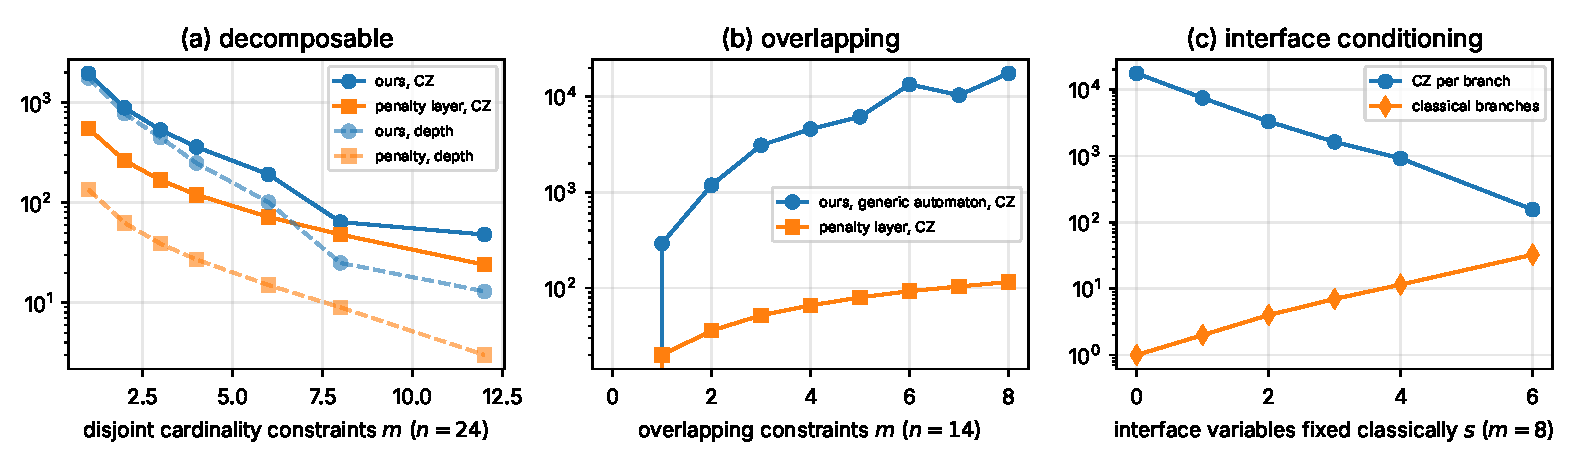
\includegraphics[width=\textwidth]{figures/constraint_scaling.pdf}\caption{\orig{exact enumeration, compiled counts, all-to-all; no noise} Cost of the feasibility block against the number of constraints. (a)~$n=24$ split in $m$ disjoint groups with exactly half of each group on: our block (Dicke per group) and the constraint phase layer of a penalty or unbalanced circuit. (b)~Random overlapping constraints (sum over five of $14$ variables at most two), generic automaton circuit with the best of six variable orders, mean of two instances. (c)~Same constraints, $m=8$: fixing $s$ variables classically lowers the CZ count per branch and increases the number of branches.}\label{fig:constraint_scaling}\end{figure*}

\paragraph{Optimising the Dicke block and the swap chain.} \orig{compiled counts; states checked against the exact one} Every block preparation starts with Dicke states, and with Qiskit's generic controlled gates they cost much more than necessary (\path{negsearch/dicke_opt.py}, \path{experiments/dicke_optimised.py}, \cref{tab:dicke_opt}). Three changes keep the state exactly (fidelity $1$ for every $n\le14$ and $k$). (i)~The doubly controlled RY as two rounds of RY, CX, RY, CX with angles $\pm\theta/4$ ($X\,\mathrm{RY}(\varphi)X=\mathrm{RY}(-\varphi)$ makes the angles add only when both controls are on): $4$ CX, which lowers the count by $32$--$40\%$. (ii)~Since the block acts only on a subspace, a least-squares fit of the whole circuit to the exact state with a three-CX template gave a closed form with $3$ CX (controls $a$, $b$, target $t$): \begin{equation*}\mathrm{RY}_t(\tfrac{\pi}{2}-\tfrac{\theta}{4})\,\mathrm{CX}_{bt}\,\mathrm{RY}_t(\tfrac{\theta}{4})\,\mathrm{CX}_{at}\,\mathrm{RY}_t(-\tfrac{\theta}{4})\,\mathrm{CX}_{bt}\,\mathrm{RY}_t(\tfrac{\theta}{4}-\tfrac{\pi}{2}),\end{equation*}verified for $n\le14$. (iii)~The decompression chain is pruned to the range that can hold a nonzero qubit, and the species with the shorter chain is the control. For a Dicke block of $12$ qubits and $6$ ones, $698\to387$ routed CZ ($-45\%$); the whole preparation of a block drops by $20$--$32\%$ ($(12,6,3)$: $917\to624$ logical CZ). The routing overhead, $1.7$--$1.9\times$, comes from the hub qubit that controls every gate of a stage. In the $120$-qubit prediction the effect is small, because its blocks have $5$ units: the preparation goes from $110$ to $96$ CZ and our light layer from $21\%$ to $22\%$ feasible shots per block, still below the unbalanced baseline ($28\%$). \emph{Negative results on the controlled-swap chain, which is $50$--$60\%$ of the preparation:} no gate cheaper than the controlled swap ($8$ CX, $7$ after optimisation) exists among classical CX and Toffoli circuits of up to five gates even with the don't-care inputs of the pruned chain; a phase-exact numerical resynthesis with up to three CX finds no exact solution (four and more did not finish; \path{experiments/cswap_resynth.py}); a three-symbol generalisation of the Dicke ladder, a network of adjacent exchanges $e^{i\theta\,\mathrm{SWAP}}$ of two units, keeps the support but its gate costs $18$ CX and it needs $18$, $28$, $74$ and $270$ exchanges for $(m,l,s)=(5,2,2)$, $(6,3,2)$, $(8,3,3)$, $(12,4,4)$ against $95$, $138$, $277$ and $666$ CX for the whole optimised preparation, i.e. $3$--$7\times$ more (\path{experiments/three_symbol_exchange.py}). A relative-phase Toffoli inside each controlled swap ($5$ CX instead of $7$) keeps the support and the magnitudes and changes the phases in multiples of $\pi/2$, lowering the preparation to $43$, $77$ and $114$ CX for $(4,2,1)$, $(5,2,2)$, $(6,3,2)$ (from $53$, $95$, $138$), but the quality of our $p=1$ layer, retrained on the actual circuit for the twelve blocks, falls from $0.669$ and $0.715$ to $0.649$ and $0.697$ (\path{experiments/retrain_relphase.py}); it is off by default (\texttt{NS\_REL\_PHASE=1}).

\begin{table*}[t]\centering\scriptsize\setlength{\tabcolsep}{3pt}
\caption{\orig{compiled counts; exact state checked for $n\le12$; nothing executed} Dicke block $|D^n_k\rangle$: CZ count and two-qubit depth, logical (all-to-all) and routed on the \texttt{ibm\_fez} coupling map (best of $10$ transpiler seeds; $6$ for $n\ge16$). ref: generic controlled gates; 4cx: hand-decomposed doubly controlled RY; 3cx: that gate with $3$ CX, exact on the states the block produces.}\label{tab:dicke_opt}
\begin{tabular}{lrrrrrr}\toprule
$(n,k)$ & logical ref & logical 3cx & routed ref & routed 4cx & routed 3cx & 2q depth ref $\to$ 3cx\\\midrule
$(6,3)$ & 73 & 45 & 116 & 65 & 58 & 110$\to$55\\
$(8,4)$ & 149 & 89 & 238 & 152 & 139 & 223$\to$119\\
$(10,5)$ & 252 & 148 & 432 & 277 & 249 & 383$\to$210\\
$(12,6)$ & 382 & 222 & 698 & 432 & 387 & 524$\to$309\\
$(16,8)$ & 723 & 415 & 1395 & 885 & 845 & 779$\to$568\\
$(24,12)$ & 1729 & 981 & 3471 & 2163 & 2034 & 1394$\to$932\\
\bottomrule\end{tabular}\end{table*}


\paragraph{Can the cost function inform the preparation?} \orig{exact simulation of the circuits; classical information from the block QUBO; no noise; nothing executed} Yes, at no cost in gates. Any state with support $F$ is a valid start, and the Dicke circuit of the preparation reaches a biased state by changing only its rotation angles: a least-squares fit of the angles to the target amplitudes $\sqrt{w(x)}$, $w=\prod_i r_i^{x_i}$ on $F$, reaches zero residual on the cases tried ($(n,k)$ up to $(6,3)$), and the CX count is that of the unbiased circuit (\path{experiments/tilted_prep.py}, \cref{tab:tilted_prep}). On the twelve blocks of the $120$-qubit instance, with the tilt $\exp(-\tau\sum_ig_ix_i)$ built from the mean-field linear field $g$ of the block and $\tau=4$, the preparation alone (the angles of the Dicke blocks, the swap chain unchanged) gives a quality among feasible samples of $0.80$ instead of $0.50$, and a probability of the block optimum of $27\%$ instead of $7\%$; the $p=1$ layer then reaches $0.85$ instead of $0.67$. A Boltzmann tilt, which needs the full cost of every feasible string, reaches $0.96$, but its smallest probability on $F$ is $4\cdot10^{-10}$, so it is an upper bound and the circuit is then a classical solution loaded into a state. Three cautions. First, the information is classical and the blocks are small ($|F|\le30$): they are solvable by enumeration, so this shows what a quantum layer can refine, not an advantage; the tilt strength $\tau$ interpolates between the exploration of the uniform state and loading a classical solution, and the best value here was at the edge of the grid. Second, the baselines profit as much. Giving the three warm-started baselines the marginals of the same tilted distribution as the start of their product state raises their quality at $p=1$ from $0.74$, $0.51$ and $0.73$ to $0.91$, $0.84$ and $0.91$ (Fourier-LCU variant, unbalanced penalty, XY mixer), above our $0.85$, with an ideal feasible fraction of $0.38$, $0.69$ and $0.33$; ours remains $1$, which is the advantage that survives, and after noise the feasible fraction of every circuit is multiplied by its ESP. Third, the angles of the Dicke blocks that realise the tilt were fitted numerically per block; a closed form for the angles from the fugacities is not derived, and the shorts are tilted through the compressed coordinates of the swap chain, so the realised state follows the target only approximately (the quality of the realised state is $0.80$ against $0.81$ of the target).
\begin{table*}[t]\centering\small
\caption{\orig{exact simulation of the logical circuits, $12$ blocks of the $120$-qubit instance; no noise; nothing executed} Cost-informed preparation. Feasible: ideal fraction of feasible samples; quality among feasible samples ($1$ is the best of the block); $P(\mathrm{opt})$: probability of the block optimum at $p=0$. Tilt: product tilt $\exp(-\tau\sum_i g_ix_i)$ with the mean-field field $g$ of the block, $\tau=4$ (edge of the grid), realised by changing only the angles of the Dicke blocks. Boltzmann: $\exp(-\tau c(x))$, an upper bound (its smallest probability on $F$ is $4\cdot10^{-10}$, so the support is exact only in name). Baselines: warm start with $k/m$ (plain) or with the marginals of the tilted distribution (biased), $p=1$.}\label{tab:tilted_prep}
\begin{tabular}{lrrrr}\toprule
preparation / method & feasible & quality $p{=}0$ & quality $p{=}1$ & $P$(opt) $p{=}0$\\\midrule
ours, uniform on $F$ & $1$ & 0.50 & 0.67 & 7\,\%\\
ours, product tilt & $1$ & 0.80 & 0.85 & 27\,\%\\
ours, Boltzmann (upper bound) & $1$ & 0.96 & 0.97 & 69\,\%\\\midrule
Fourier-LCU variant, plain & 0.24 & -- & 0.74 & --\\
Fourier-LCU variant, biased & 0.38 & -- & 0.91 & --\\
unbalanced penalty, plain & 0.59 & -- & 0.51 & --\\
unbalanced penalty, biased & 0.69 & -- & 0.84 & --\\
XY mixer, plain & 0.24 & -- & 0.73 & --\\
XY mixer, biased & 0.33 & -- & 0.91 & --\\
\bottomrule\end{tabular}\end{table*}



\section{A 120-qubit experiment: specification, prediction and criteria}\label{app:hw100}
The estimates of \cref{sec:sota} concern one core at a time. To use a chip of more than $100$ qubits we use the independence that the interface gives: a portfolio of $10$ assets, $6$ periods and $2$ sectors ($n=120$ variables, a looser family with at least $10$ feasible strings per block, \path{negsearch/hw100.py}) splits into twelve blocks of $10$ qubits, each with its own quadratic objective (the neighbours enter as linear fields), and the twelve blocks are placed on disjoint connected regions of $11$ physical qubits and run as one circuit of $120$ measured qubits and $120$ classical bits (a chip with at least $132$ usable qubits, such as the $156$-qubit \texttt{ibm\_fez}). Twelve circuits are specified: our light and full $p=1$ layers, our preparation alone, a Hadamard control, three baselines from the warm-started product state of the Fourier-LCU paper (single-basis Fourier-LCU, unbalanced penalty, XY-mixer QAOA; trained by exact simulation, with the same decomposition and count constraints, the setting most favourable to them) and the five cost-informed circuits of \cref{sec:core}. \Cref{tab:hw100_pred,tab:hw100_cost} give the compiled counts, depths and the noise-model prediction (\cref{sec:sota}). A complete shot is feasible with probability roughly the product of the block probabilities, so the useful output is the per-block post-selected samples, assembled into feasible assignments of all $120$ variables. The pre-stated criteria are: (1)~the preparation is above the upper $95\%$ bound of the control; (2)~preparation and light layer are above the upper bounds of the three baselines, and (2c)~the tilted preparation is above the three baselines that receive the same classical information; (3)~all twelve blocks return at least $50$ accepted samples for the preparation; (4)~the light layer has higher quality than the preparation alone; (5)~the measured feasibility of the preparation is within $0.1$ of the prediction. Criterion 2 is predicted to hold for the preparation (and 2c for the tilted one) and to fail for the light layer against the unbalanced circuit, criterion 4 may fail, and the comparison of the quality of the tilted preparation with the biased baselines (4b) is predicted to fail ($0.79$ against $0.83$--$0.88$); the comparison of quality with the baselines is reported, not required. What the experiment would show is feasibility by construction at a scale at which the global-constraint methods have no chance, with the baselines given the decomposition; it would not show a quantum advantage, since blocks of ten qubits are classically trivial, nor better optimisation inside the blocks. The notebooks (\path{notebooks/HW100_*.ipynb}) run the same analysis on the noise model, on a gate-level simulation of each block, or on a device.

\begin{table*}[t]\centering\scriptsize\setlength{\tabcolsep}{3pt}
\caption{\orig{compiled counts, uniform error model $e_2=0.0035$ per two-qubit gate; no noise simulation, nothing executed} One block of the $120$-qubit portfolio ($(l,s)=(2,1)$, $|F|=30$, 10 qubits) compiled to different connectivities with CZ as the only two-qubit gate. Entries: two-qubit gates / two-qubit depth / ESP, best of six transpiler seeds. Preparation: our preparation alone; layer: our light $p=1$ layer (\texttt{architectures.py}; a second block gives the same pattern).}\label{tab:arch}
\begin{tabular}{lcccc}\toprule
topology & our prep. & our layer & Fourier-LCU / unbalanced & XY mixer\\
\midrule
all-to-all & 90 / 64 / 0.66 & 215 / 118 / 0.38 & 90 / 34 / 0.68 & 106 / 36 / 0.62\\
grid $2{\times}5$ & 131 / 90 / 0.56 & 333 / 181 / 0.23 & 112 / 42 / 0.60 & 126 / 44 / 0.56\\
ring & 168 / 110 / 0.49 & 393 / 227 / 0.18 & 152 / 71 / 0.51 & 178 / 74 / 0.45\\
heavy-hex patch & 190 / 164 / 0.44 & 415 / 251 / 0.16 & 140 / 77 / 0.53 & 177 / 85 / 0.45\\
line & 196 / 164 / 0.43 & 418 / 242 / 0.16 & 152 / 75 / 0.51 & 180 / 70 / 0.44\\
\bottomrule\end{tabular}\end{table*}

\paragraph{Does the architecture matter?} \orig{compiled counts, uniform error model; no noise simulation} \Cref{tab:arch} compiles one block to five connectivities (\path{experiments/architectures.py}). The baselines' circuits are a product-state layer followed by one $ZZ$ layer, so their cost moves from $90$ two-qubit gates (all-to-all) to $112$--$152$ on sparse devices ($1.2$--$1.7\times$). Our preparation is more sensitive to connectivity: for the block shown it goes from $90$ (all-to-all) to $131$ on a $2\times5$ grid, $168$ on a ring and $190$ on a heavy-hex patch ($2.1\times$), because the controlled-swap chain moves units across the block; our light layer goes from $215$ to $333$ on the grid and $415$ on heavy-hex. So the ratio of our layer to the baselines is $2.4\times$ all-to-all and $2.7$--$3.0\times$ on heavy-hex, and higher connectivity (a grid or all-to-all) would lower our ESP penalty more than theirs: ESP of the layer $0.16$ (heavy-hex) against $0.23$ (grid) and $0.38$ (all-to-all), against $0.53$, $0.60$ and $0.68$ for the baselines. A native fractional $R_{ZZ}$ gate halves the baselines on all-to-all ($45$ against $90$) but changes ours by only $19\%$ ($175$ against $215$) and the sparse cases little, since routing dominates there; we did not model its error. Smaller preparations, with $|F|=10$, are nearly topology-independent ($23$--$29$ gates), so the sensitivity grows with the number of units in the block. These counts bound what a different architecture (or a better layout for the Dicke hub) could give; the conclusions of the paper concern the heavy-hex Heron devices.

\section{Inequality constraints in QAOA: QOBLIB portfolio optimisation}\label{sec:portfolio}
This appendix uses the constraint automaton to encode \emph{inequality} constraints in QAOA~\cite{farhi2014,hadfield2019}, on class \texttt{06-portfolio} of the Quantum Optimization Benchmarking Library (QOBLIB)~\cite{koch2026qoblib}.

\paragraph{Model.} At each period $t$ the investor holds long and short positions $x_{t,d,i}\in\{0,1\}$ ($d\in\{\mathrm{long},\mathrm{short}\}$, one unit per asset, \texttt{ub}$=1$). The objective (risk, return, transaction, short-selling and liquidation costs, cash interest) is the reference model \texttt{bqp\_u3\_c10}; our implementation reproduces the official QOBLIB checker exactly, including the reference value $-1595$ of the ISQR submission for \texttt{po\_a003\_t02\_orig}. Each period has two inequalities, $0\le C-(L_t-S_t)\le 2^{c_1}-1$ (capital) and $0\le B-(L_t+S_t)\le 2^{c_2}-1$ (budget), where $L_t,S_t$ count long and short positions. We use $C=3$, $B=3$ or $4$, and the risk weights of the ISQR submission ($10^{-5}$--$4\cdot10^{-5}$) or a QOBLIB \texttt{l1e-5} variant. This is a derived model, not the QOBLIB reference variant (three units, $C=10$), so optimal values are not comparable with the QOBLIB table. Exact optima and worst feasible values come from a dynamic programme over periods.

\paragraph{Encodings compared.} (i) The official QUBO, with $T(c_1+c_2)$ binary slack qubits and a quadratic penalty. (ii) Unbalanced penalisation~\cite{montanez2024unbalanced}, which needs no slack qubits. (iii) The negation-forced state $A_q|0\rangle$ as initial state: a variable is forced when its other value would make the period's constraints impossible to complete (exact look-ahead on the counters $(L,S)$), so the support is exactly the feasible set and there are no dead ends. It is combined with the X mixer, with an XY mixer~\cite{wang2020xy} inside each (period, direction) block, which conserves $L_t$ and $S_t$ and hence feasibility, or with the Grover mixer about $A_q|0\rangle$~\cite{bartschi2020gm} (CG-QAOA). With (iii) the phase operator contains only the objective, without any penalty term. \Cref{fig:hybrid} shows the hybrid circuit.

\begin{figure*}[t]\centering
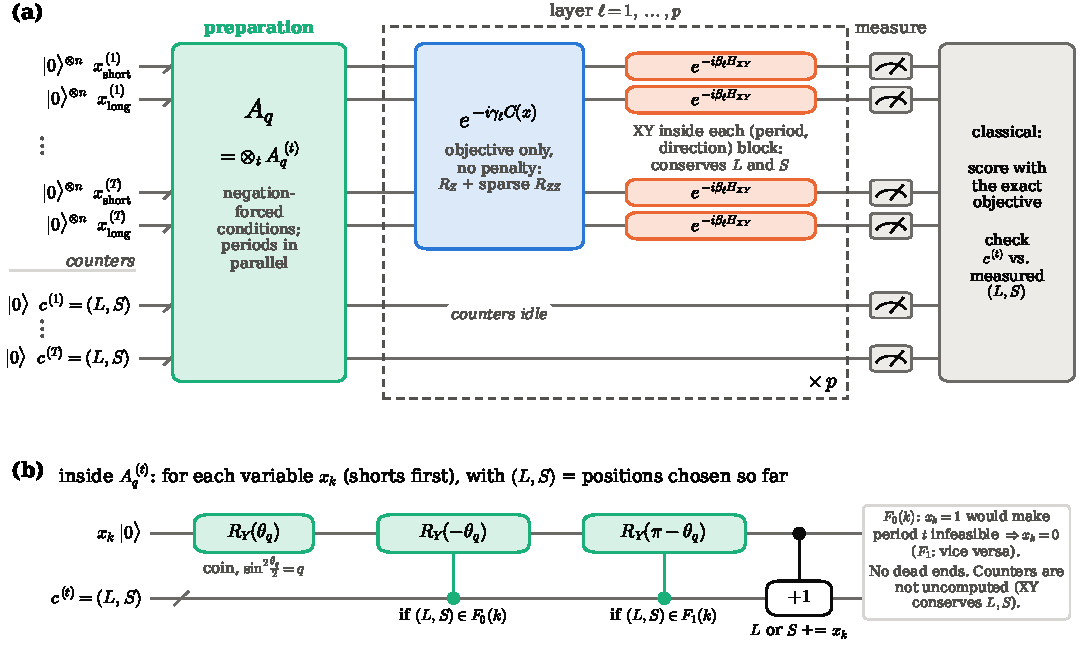
\includegraphics[width=\textwidth]{figures/fig_hybrid_blocks.pdf}
\caption{Hybrid constraint-guided QAOA. (a) Inequalities are enforced once by $A_q=\bigotimes_t A_q^{(t)}$ (periods in parallel); each layer applies the objective-only phase and an XY mixer inside each (period, direction) block, which conserves $(L,S)$. (b) One variable inside $A_q^{(t)}$: coin $R_Y(\theta_q)$, counter-controlled correction when $x_k$ is forced to 0 ($F_0$) or 1 ($F_1$), counter increment. Counters need no uncomputation because XY conserves the counts.}\label{fig:hybrid}
\end{figure*}

\paragraph{Exact simulation.} \Cref{tab:pf_exact,fig:pf_quality} report $p=1,2,3$ on three QOBLIB instances (12, 16, 20 decision qubits). Penalty weights are tuned over $\alpha\in[1/64,8]$ times the largest linear coefficient, and the best value is kept. Five observations: (1)~$A_q$ followed by the X mixer leaks out of the feasible set and ends below $A_q$ alone at every depth: \emph{the constraint-guided state helps only with a constraint-preserving mixer}. (2)~The hybrid ($A_q$ + XY) is 100\,\% feasible and has higher quality and higher P(optimum) than both penalty encodings at every depth on every instance. (3)~CG-QAOA is best in quality and P(optimum). (4)~If infeasible samples are discarded classically, the surviving penalty samples are as good as or better than the hybrid's on the two smaller instances: the hybrid's gain on these two instances is only that it does not waste shots on infeasible samples. (5)~$A_q$ alone is classically samplable and already strong; the QAOA layers add up to $13\times$ in P(optimum) on top of it.

\begin{figure*}[t]\centering
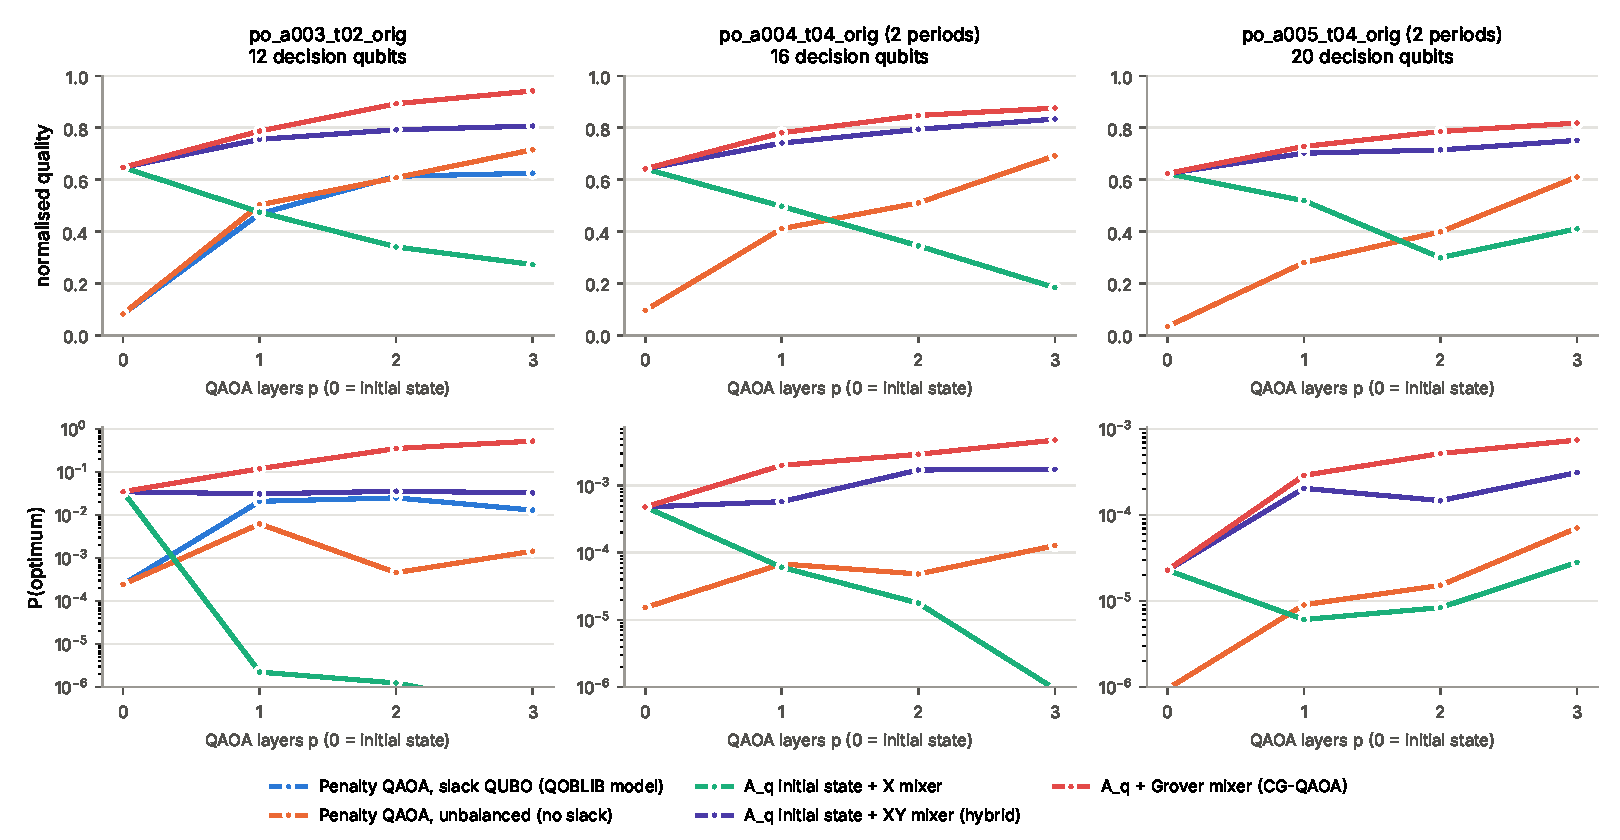
\includegraphics[width=0.92\textwidth]{figures/fig_portfolio_quality.pdf}
\caption{\orig{exact ideal simulation} Exact simulation, QOBLIB portfolio instances: normalised quality (infeasible = 0) and P(optimum) vs.\ QAOA depth. $p=0$ is the initial state.}\label{fig:pf_quality}
\end{figure*}
\begin{table*}[t]\centering\small
\caption{\orig{exact ideal simulation} Exact simulation on QOBLIB portfolio instances: P(feasible) / normalised quality (infeasible samples count 0) / P(optimum) for $p=1,2,3$. Penalty weights tuned over $\alpha\in[1/64,8]$; best value kept. $p=0$: uniform sampling (penalty rows) or $A_q$ alone (classically samplable).}\label{tab:pf_exact}
\resizebox{\linewidth}{!}{\begin{tabular}{llcccc}\toprule instance (qubits ours/slack) & method & $p=0$ & $p=1$ & $p=2$ & $p=3$\\\midrule
\texttt{a003\_t02} (12/20) & Penalty, slack QUBO & 0.17 / 0.08 / 2.4e-4 & 0.58 / 0.47 / 2.1e-2 & 0.72 / 0.61 / 2.5e-2 & 0.77 / 0.62 / 1.3e-2\\
 & Penalty, unbalanced & 0.17 / 0.08 / 2.4e-4 & 0.63 / 0.50 / 6.2e-3 & 0.79 / 0.61 / 4.6e-4 & 0.81 / 0.72 / 1.4e-3\\
 & $A_q$ + X mixer & 1.00 / 0.65 / 3.5e-2 & 0.96 / 0.47 / 2.2e-6 & 0.70 / 0.34 / 1.2e-6 & 0.57 / 0.27 / 3.0e-7\\
 & $A_q$ + XY (hybrid) & 1.00 / 0.65 / 3.5e-2 & 1.00 / 0.76 / 3.1e-2 & 1.00 / 0.79 / 3.6e-2 & 1.00 / 0.81 / 3.3e-2\\
 & $A_q$ + Grover (CG-QAOA) & 1.00 / 0.65 / 3.5e-2 & 1.00 / 0.79 / 1.2e-1 & 1.00 / 0.89 / 3.5e-1 & 1.00 / 0.94 / 5.3e-1\\
\midrule
\texttt{a004\_t04} (2 per.) (16/26) & Penalty, unbalanced & 0.17 / 0.10 / 1.5e-5 & 0.56 / 0.41 / 6.8e-5 & 0.61 / 0.51 / 4.8e-5 & 0.81 / 0.69 / 1.3e-4\\
 & $A_q$ + X mixer & 1.00 / 0.64 / 4.8e-4 & 0.81 / 0.50 / 6.1e-5 & 0.55 / 0.34 / 1.8e-5 & 0.29 / 0.18 / 9.4e-7\\
 & $A_q$ + XY (hybrid) & 1.00 / 0.64 / 4.8e-4 & 1.00 / 0.74 / 5.8e-4 & 1.00 / 0.79 / 1.7e-3 & 1.00 / 0.83 / 1.7e-3\\
 & $A_q$ + Grover (CG-QAOA) & 1.00 / 0.64 / 4.8e-4 & 1.00 / 0.78 / 2.0e-3 & 1.00 / 0.85 / 2.9e-3 & 1.00 / 0.88 / 4.8e-3\\
\midrule
\texttt{a005\_t04} (2 per.) (20/30) & Penalty, unbalanced & 0.06 / 0.03 / 9.5e-7 & 0.43 / 0.28 / 9.0e-6 & 0.55 / 0.40 / 1.5e-5 & 0.84 / 0.61 / 7.1e-5\\
 & $A_q$ + X mixer & 1.00 / 0.62 / 2.3e-5 & 0.87 / 0.52 / 6.1e-6 & 0.48 / 0.30 / 8.4e-6 & 0.68 / 0.41 / 2.8e-5\\
 & $A_q$ + XY (hybrid) & 1.00 / 0.62 / 2.3e-5 & 1.00 / 0.70 / 2.0e-4 & 1.00 / 0.71 / 1.5e-4 & 1.00 / 0.75 / 3.1e-4\\
 & $A_q$ + Grover (CG-QAOA) & 1.00 / 0.62 / 2.3e-5 & 1.00 / 0.73 / 2.9e-4 & 1.00 / 0.79 / 5.2e-4 & 1.00 / 0.82 / 7.4e-4\\
\bottomrule\end{tabular}}\end{table*}


\paragraph{Reducing depth.} \Cref{tab:pf_depth} follows the hybrid through four versions on \texttt{ibm\_fez}. v1 (counters uncomputed) costs 511--1857 CZ at $p=1$ and the Grover mixer 4\,000--13\,000 CZ per layer, beyond current devices. v2 orders the shorts first, which leaves fewer forced counter states, and keeps one counter pair per period without uncomputation; the counters then hold $(L_t,S_t)$, which XY conserves, so all statistics on $x$ are unchanged (verified against the exact state). This halves $A_q$ (324$\to$150 CZ on 12 qubits). v3 drops the small risk couplings from the phase and uses XY on a path. Constraints sit in the state, not in the cost, so this does not lower the ideal quality, whereas a penalty is quadratic by construction. Together v1$\to$v3 removes 65--75\,\% of the CZ gates and 75--82\,\% of the depth. Off-the-shelf ZX simplification did not help here: PyZX \texttt{full\_reduce} with extraction roughly doubles the CZ count and phase teleportation is neutral (within 8\,\%). Comparing all-to-all with heavy-hex compilation shows that about 40\,\% of the remaining CZ gates are routing, which architecture-aware synthesis could target.

\paragraph{Classicality as a design tool.} Feasibility depends only on the counts $(L_t,S_t)$, because every unit has the same cash value, and neither XY nor the phase changes them. Different count sectors therefore never interfere, and the logic of the negative conditions can be executed classically, which is an instance of the idea behind the classicality lemma (\cref{sec:classical}). Draw $(L_t,S_t)$ per shot from the weights of $A_q$, either offline or with a mid-circuit-measured coin, and let the chip prepare only the superposition over \emph{which} assets, a Dicke state per block~\cite{bartschi2019dicke}, followed by the XY layers. Measuring the decision qubits themselves, by contrast, destroys the gain (quality $0.76\to0.64$). The same statistics are obtained coherently and without ancillas: a weighted ``thermometer'' state of the counts followed by the Dicke unitary $U_{n,k}$ of Ref.~\cite{bartschi2019dicke}, which we verified to coincide exactly with the per-shot construction. With counts drawn per shot the 12-qubit circuit needs 24 (40) CZ at $p=1$ ($p=2$) instead of 178 (200), with quality 0.74 (0.84).

\begin{table}[t]\centering\small
\caption{\orig{compiled counts} CZ gates / depth on \texttt{ibm\_fez} (FakeFez, level 3) for one and two layers. v1: counters uncomputed; v2: shorts-first order, lean counters; v3: v2 + path XY + linear phase; counts+Dicke: counts drawn classically, Dicke preparation (most expensive count sector).}\label{tab:pf_depth}
\resizebox{\linewidth}{!}{\begin{tabular}{lccc}\toprule circuit & a003 (12) & a004 (16) & a005 (20)\\\midrule
penalty, slack QUBO, $p=1$ & 311/312 & 588/460 & 854/664\\
penalty, unbalanced, $p=1$ & 92/128 & 185/184 & 301/279\\
hybrid v1, $p=1$ & 511/952 & 1323/2291 & 1857/3053\\
hybrid v2, $p=1$ & 330/387 & 762/696 & 1064/936\\
hybrid v3, $p=1$ & 178/225 & 446/567 & 541/652\\
counts+Dicke, $p=1$ & 24/32 & 156/127 & --\\
\midrule
penalty, slack QUBO, $p=2$ & 693/639 & 1231/986 & 1863/1219\\
penalty, unbalanced, $p=2$ & 206/258 & 408/422 & 674/610\\
hybrid v1, $p=2$ & 678/1361 & 1618/2982 & 2400/3456\\
hybrid v2, $p=2$ & 481/567 & 1100/1040 & 1617/1635\\
hybrid v3, $p=2$ & 200/255 & 454/528 & 601/690\\
counts+Dicke, $p=2$ & 40/49 & 184/148 & --\\
\midrule
CG-QAOA (Grover mixer), $p=1$ & 4013/9882 & 9203/20872 & 13364/31631\\
\bottomrule\end{tabular}}\end{table}


\paragraph{Noise.} \Cref{tab:pf_noise,fig:pf_noise} use the \texttt{ibm\_fez} noise model on \texttt{po\_a003\_t02\_orig}. Feasibility is no longer guaranteed, and the first hybrid (531 CZ) is worse than unbalanced penalty QAOA. The hardware-friendly versions reverse this: counts+Dicke reaches quality 0.70--0.75 with 27--52 CZ per shot, against at most 0.50 for any penalty circuit, and P(optimum) 4.5\,\% against at most 1\,\%.

\begin{table}[t]\centering\small
\caption{\orig{gate-level noisy simulation (FakeFez noise model); no hardware} \texttt{po\_a003\_t02\_orig} under the \texttt{ibm\_fez} noise model (FakeFez, 2000--4000 shots).}\label{tab:pf_noise}
\resizebox{\linewidth}{!}{\begin{tabular}{lcccc}\toprule circuit & CZ & P(feas.) & quality & P(opt)\\\midrule
penalty, unbalanced, $p=1$ & 101 & 0.60 & 0.47 & 0.8\%\\
penalty, slack, $p=1$ & 339 & 0.47 & 0.36 & 0.9\%\\
penalty, unbalanced, $p=2$ & 206 & 0.68 & 0.50 & 0.1\%\\
penalty, slack, $p=2$ & 693 & 0.52 & 0.39 & 1.0\%\\
$A_q$ alone (lean, classically samplable) & 150 & 0.92 & 0.59 & 2.1\%\\
hybrid v1, $p=1$ & 531 & 0.59 & 0.39 & 1.4\%\\
hybrid v3, $p=1$ & 178 & 0.85 & 0.63 & 2.4\%\\
hybrid v3, $p=2$ & 200 & 0.80 & 0.63 & 1.0\%\\
counts+Dicke, $p=1$ & 27 & 0.95 & 0.70 & 4.5\%\\
counts+Dicke, $p=2$ & 52 & 0.90 & 0.75 & 1.2\%\\
\bottomrule\end{tabular}}\end{table}

\begin{figure}[t]\centering
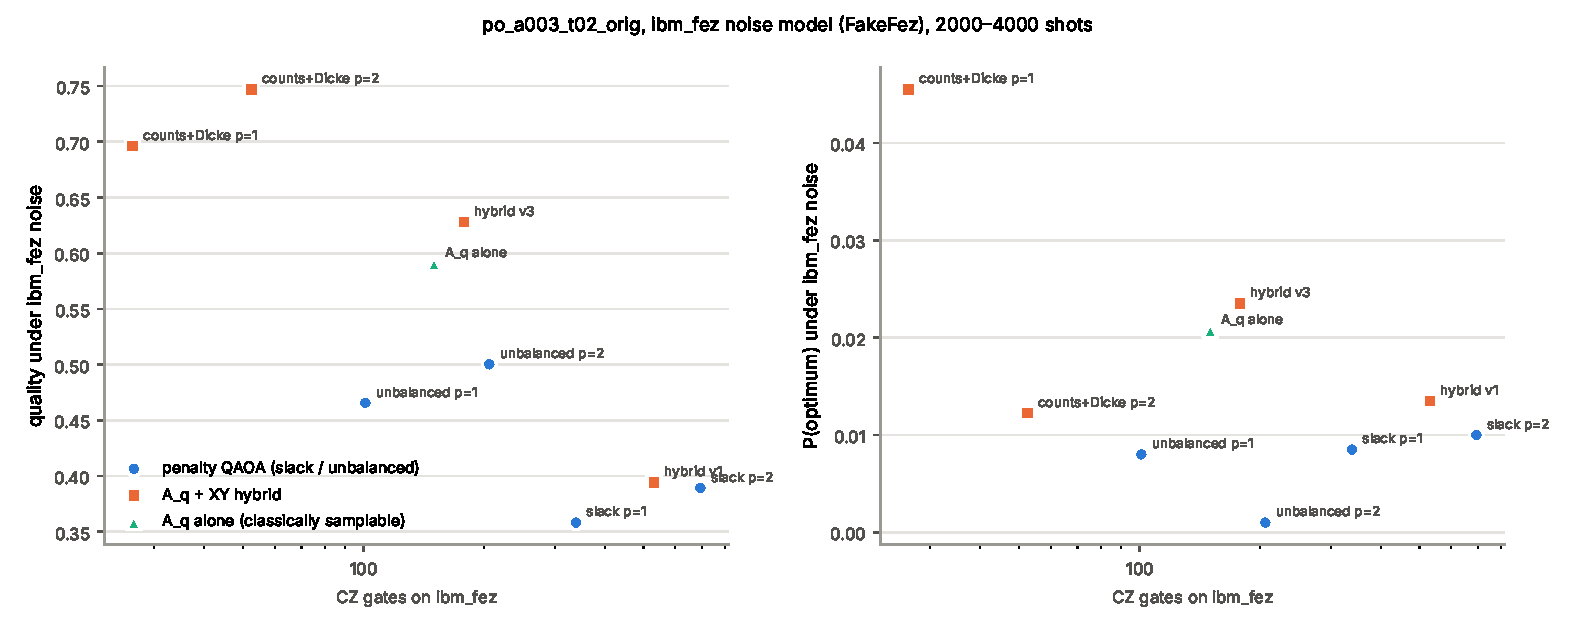
\includegraphics[width=\columnwidth]{figures/fig_portfolio_noisy.pdf}
\caption{\orig{gate-level noisy simulation; no hardware} Quality and P(optimum) vs.\ CZ count under the \texttt{ibm\_fez} noise model (\texttt{po\_a003\_t02\_orig}).}\label{fig:pf_noise}
\end{figure}

\paragraph{Scaling to 300 qubits.} \Cref{tab:pf_scaling,fig:pf_scaling} use Qiskit Aer's MPS simulator on seven QOBLIB instances, from 12 to 300 decision qubits (\texttt{a003\_t02} to \texttt{a010\_t15}), at $p=1$. Angles were transferred from the exactly optimised small instances (phase in units of the largest linear coefficient) and refined on a grid. Bond dimension 64 agrees with 256 and, on 12 qubits, with the exact statevector. The fair classical baseline draws the same counts and a uniform subset of assets. Unbalanced penalty QAOA falls from 64\,\% feasible samples to 0 of 2000 at 300 qubits; the hybrid stays at 100\,\%. It exceeds the classical baseline in quality by 0.04--0.15 at every size, and its best of 2000 shots is 1.2--4.8 times closer to the exact optimum. Where the circuits fit on \texttt{ibm\_fez}, the per-shot hybrid is the cheapest, and the single coherent circuit is cheaper than the penalty circuit from 80 qubits on.

\begin{figure*}[t]\centering
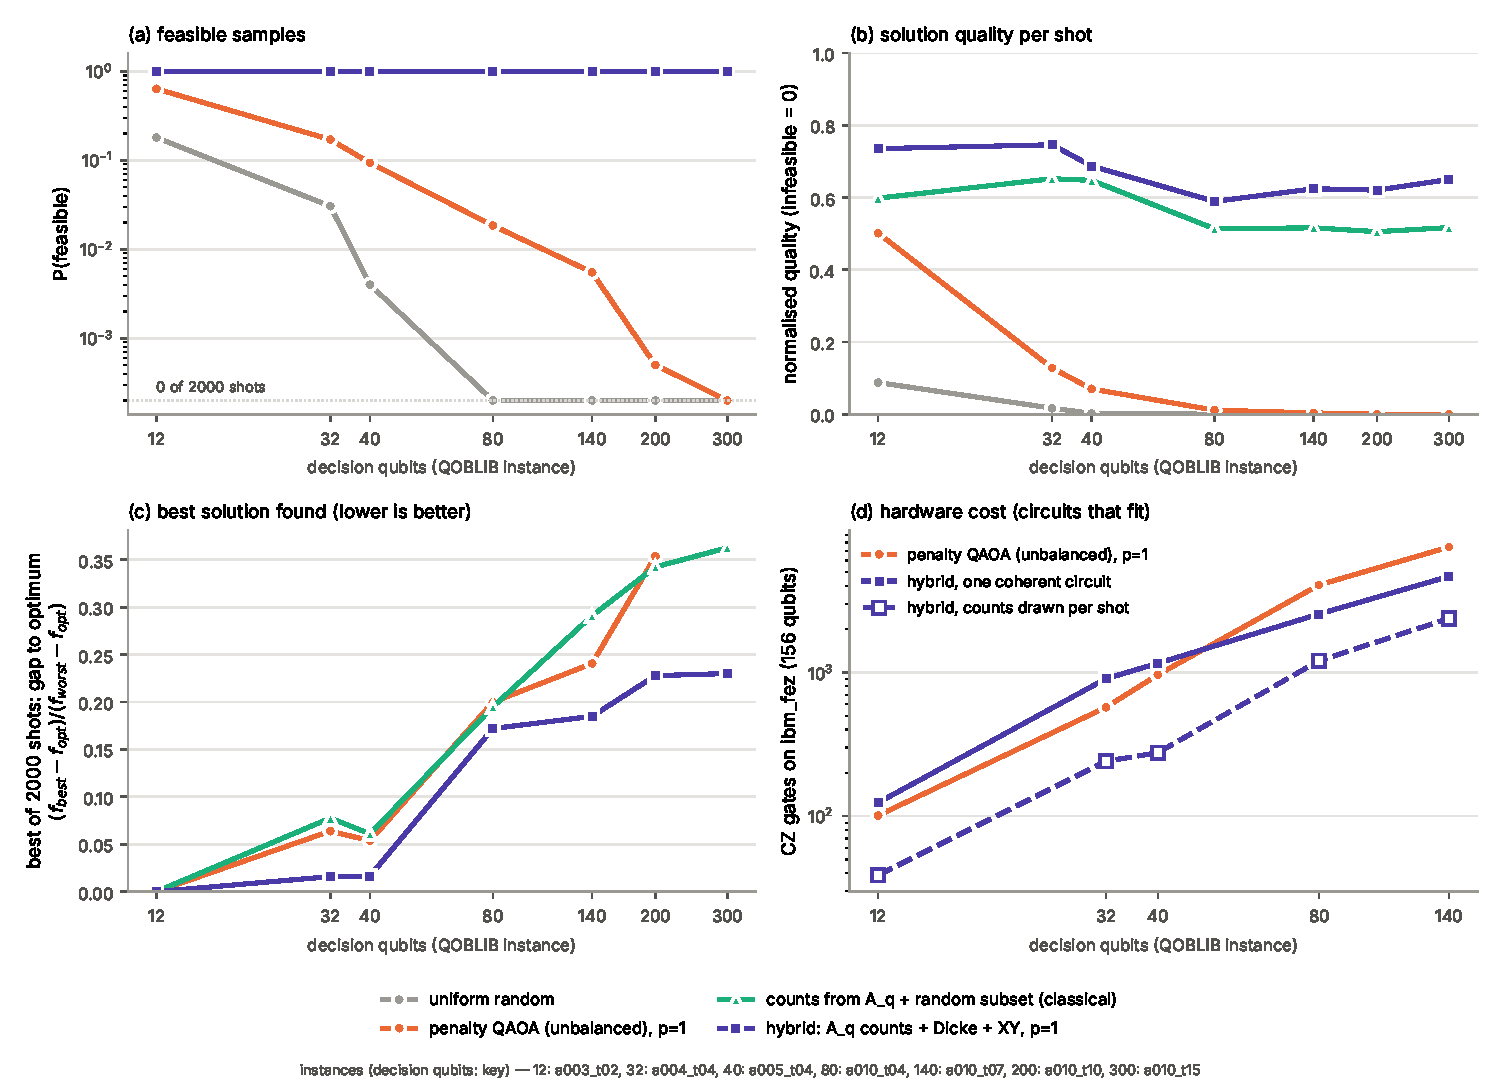
\includegraphics[width=0.9\textwidth]{figures/fig_portfolio_scaling.pdf}
\caption{\orig{ideal matrix-product-state simulation and compiled counts} QOBLIB portfolio instances from 12 to 300 decision qubits (Aer MPS, $p=1$, 2000 shots): feasibility, quality, best-shot gap to the exact optimum, and CZ count on \texttt{ibm\_fez}.}\label{fig:pf_scaling}
\end{figure*}
\begin{table*}[t]\centering\small
\caption{\orig{ideal matrix-product-state simulation and compiled counts} Aer MPS simulation (bond dimension 64), $p=1$, 2000 shots. Quality: normalised, infeasible = 0; gap: best of 2000 shots, $(f_{best}-f_{opt})/(f_{worst}-f_{opt})$, exact $f_{opt}$ by dynamic programming. CZ on \texttt{ibm\_fez} only where the circuit fits (156 qubits).}\label{tab:pf_scaling}
\resizebox{\linewidth}{!}{\begin{tabular}{lrrcccccccc}\toprule & & & \multicolumn{2}{c}{P(feasible)} & \multicolumn{3}{c}{quality} & \multicolumn{2}{c}{best-shot gap} & CZ (pen./hyb./per shot)\\
instance & qubits & slack QUBO & pen. & hyb. & pen. & classical & hyb. & classical & hyb. & \\\midrule
\texttt{a003\_t02} & 12 & 20 & 0.6355 & 1 & 0.501 & 0.598 & 0.735 & 0.000 & 0.000 & 101/124/39\\
\texttt{a004\_t04} & 32 & 52 & 0.1710 & 1 & 0.128 & 0.652 & 0.746 & 0.078 & 0.016 & 572/904/241\\
\texttt{a005\_t04} & 40 & 60 & 0.0935 & 1 & 0.070 & 0.648 & 0.687 & 0.061 & 0.016 & 963/1158/276\\
\texttt{a010\_t04} & 80 & 100 & 0.0185 & 1 & 0.011 & 0.514 & 0.589 & 0.195 & 0.172 & 4056/2546/1205\\
\texttt{a010\_t07} & 140 & 175 & 0.0055 & 1 & 0.004 & 0.516 & 0.625 & 0.291 & 0.185 & 7452/4655/2376\\
\texttt{a010\_t10} & 200 & 250 & 0.0005 & 1 & 0.000 & 0.505 & 0.621 & 0.342 & 0.228 & --\\
\texttt{a010\_t15} & 300 & 375 & 0.0000 & 1 & 0.000 & 0.517 & 0.650 & 0.363 & 0.230 & --\\
\bottomrule\end{tabular}}\end{table*}


\paragraph{Limitations of this study.} (i)~With a linear phase and XY on paths, entanglement stays inside blocks of $n$ qubits. That is why MPS scales, and it also means this regime is classically simulable: we claim a better \emph{encoding}, not a quantum advantage, and classical MIQP solvers solve all these instances~\cite{babbush2021}. (ii)~The counts trick needs constraints that depend only on counts. Weighted constraints (multiple knapsack) need the coherent $A_q$ with counters, or the indicator oracles of Ref.~\cite{bucher2025}. (iii)~Most of the gain comes from the count distribution, which is classical; the quantum layers add a consistent but moderate improvement. (iv)~The noise results are simulations of a noise model and cover one instance; no device run is reported. (v)~Angles at large sizes come from transfer plus a grid, not a full optimisation. (vi)~The model is a derived QOBLIB variant (\texttt{ub}$=1$).

\section{Measure-and-flip dynamic circuits are classical}\label{sec:classical}
\begin{lemma}[Classicality]\label{lem:classical}
Consider a circuit on qubits initialised to $|0\rangle$, with a layer of Hadamards on a subset $S$, followed by any sequence of (i)~permutation gates in the computational basis (X, CNOT, Toffoli, multi-controlled X), (ii)~diagonal gates, (iii)~computational-basis measurements and resets, and (iv)~classically controlled versions of (i)--(iii). The joint distribution of all measurement outcomes equals that of the classical algorithm that samples the bits in $S$ uniformly and applies (i), (iii), (iv) to bit strings.
\end{lemma}
\begin{proof}
Let $\Delta$ be complete dephasing in the computational basis. For a permutation $P$ and a diagonal unitary $D$, $\Delta(P\rho P^\dagger)=P\Delta(\rho)P^\dagger$ and $\Delta(D\rho D^\dagger)=\Delta(\rho)$; computational-basis measurement and reset commute with $\Delta$, and so do their classically controlled versions. Hence inserting $\Delta$ right after the Hadamard layer does not change any outcome statistics. Since $\Delta(|{+}\rangle\langle{+}|)=\mathbb{1}/2$, the state after dephasing is a uniform mixture over bit strings on $S$, evolved by permutations and measurements, i.e. a classical randomized algorithm.
\end{proof}
The lemma also applies at block level: a quantum adder acting on a register initialised to $|0\rangle$ is a permutation of basis states even if implemented with QFT rotations. \Cref{tab:classical} confirms the lemma on the two original proposals: a measure-and-flip 2-colouring of path graphs (simulated with the stabilizer method, $n$ up to 60) and a measure-and-flip subset-sum circuit with a QFT adder.

\begin{table}[t]\centering\small
\caption{Classicality check (Lemma~\ref{lem:classical}): success probability of the measure-and-flip circuits (stabilizer simulation, 50\,000 shots) versus the same rules executed classically ($2\times10^6$ trials); all differences are within $2\sigma$ of shot noise.}\label{tab:classical}
\begin{tabular}{lrrr}\toprule Circuit & iters & quantum & classical\\\midrule
2-col path P10 & 2 & 0.0086 & 0.0078\\
2-col path P10 & 5 & 0.0624 & 0.0624\\
2-col path P10 & 10 & 1.0000 & 1.0000\\
2-col path P10 & 20 & 1.0000 & 1.0000\\
2-col path P30 & 7 & 0.0000 & 0.0000\\
2-col path P30 & 15 & 0.0001 & 0.0001\\
2-col path P30 & 30 & 1.0000 & 1.0000\\
2-col path P30 & 60 & 1.0000 & 1.0000\\
2-col path P60 & 15 & 0.0000 & 0.0000\\
2-col path P60 & 30 & 0.0000 & 0.0000\\
\midrule \multicolumn{4}{l}{Subset sum $\{1,2,3,4\}$, target 7, QFT adder: TV distance 0.0008}\\
\bottomrule\end{tabular}
\end{table}

\section{Negation-forced preparation for CNF formulas}\label{sec:nf}
The main text builds the state $A_q$ from a general constraint automaton. This appendix is the original special case that motivated it: for a CNF formula, a clause is the negation of a forbidden pattern, and ``all other literals false'' is the condition that forces a variable. It gives the exact success probability, the PPZ-type gate bound and the ZX and fault-tolerant analyses below.
Let $F$ be a CNF formula over $x_1,\dots,x_n$ and $\pi$ an order of the variables.
\begin{definition}[Negative conditions]
For a variable $v$, let $\mathcal C_1(v)$ ($\mathcal C_0(v)$) be the clauses containing the literal $v$ ($\neg v$) whose other variables all precede $v$ in $\pi$. Given an assignment of the preceding variables, $v$ is \emph{forced to 1} (resp.\ 0) if some clause in $\mathcal C_1(v)$ ($\mathcal C_0(v)$) has all its other literals false. $\mathcal C^{K}$ keeps at most $K$ clauses of each polarity.
\end{definition}
\begin{definition}[In-place preparation $A_\pi^K$]
Process the variables in order $\pi$. For $v$: compute the flags $f_1,f_0$ (OR over clauses of the AND of their negated other literals), apply $\mathrm{CNOT}(f_1\!\to\!x_v)$, apply a Hadamard on $x_v$ controlled on $\neg f_1\wedge\neg f_0$, then uncompute the flags. All work qubits return to $|0\rangle$.
\end{definition}
The variable qubit is its own coin; no register of random choices and no history is stored. The circuit uses only Toffoli, controlled-Hadamard, CNOT and X gates (\cref{alg:prep}); the number of Toffolis is $O(\sum_v |\mathcal C(v)|\,k)=O(km)$.

\begin{algorithm}[t]
\caption{Negation-forced preparation $A^K_\pi$}\label{alg:prep}
\begin{algorithmic}[1]
\For{$v$ in order $\pi$}
\For{$c\in\mathcal C_1^K(v)\cup\mathcal C_0^K(v)$}
\State $a_c \gets \bigwedge_{\ell\in c\setminus\{v\}} \neg\ell$ \Comment{negative condition}
\EndFor
\State $f_1\gets\bigvee_{c\in\mathcal C_1}a_c$;\; $f_0\gets\bigvee_{c\in\mathcal C_0}a_c$
\State $x_v \mathrel{\oplus}= f_1$;\; \textbf{if} $\neg f_1\wedge\neg f_0$ \textbf{then} $H(x_v)$ \Comment{decision}
\State uncompute $f_1,f_0,a_c$
\EndFor
\end{algorithmic}
\end{algorithm}

\begin{figure}[t]\centering
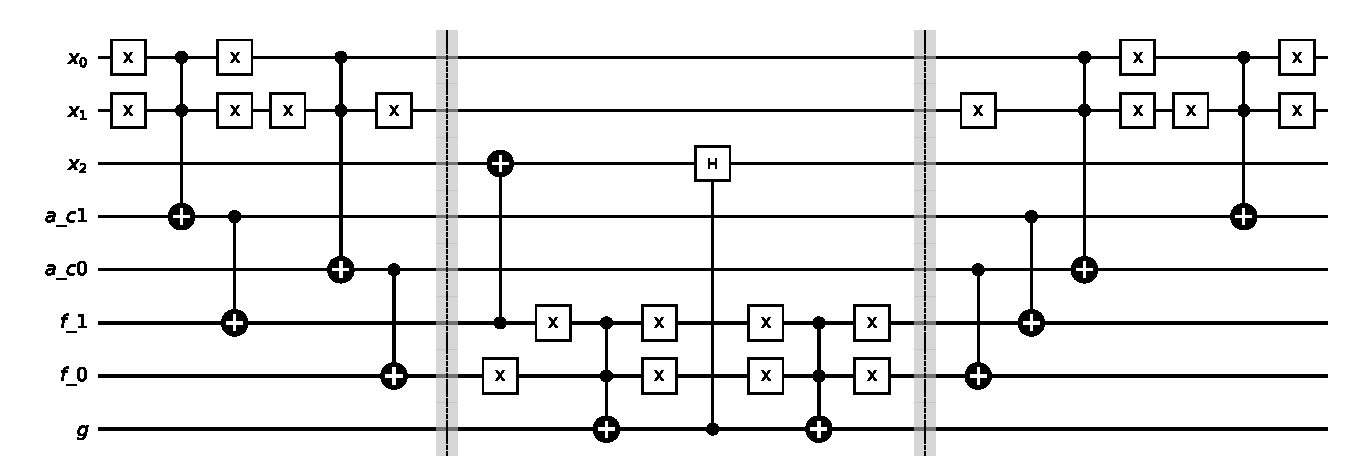
\includegraphics[width=\columnwidth]{figures/fig_step.pdf}
\caption{One negation-forced step for variable $x_2$ with clauses $(x_0\vee x_1\vee x_2)\in\mathcal C_1$ and $(\neg x_0\vee x_1\vee\neg x_2)\in\mathcal C_0$. Left: negative conditions $a_c$ (all other literals false) and flags $f_1,f_0$. Middle: forced value and the decision (controlled Hadamard on the variable itself). Right: uncomputation; all ancillas return to $|0\rangle$ and are reused for the next variable.}
\label{fig:step}
\end{figure}

\begin{lemma}[Soundness]\label{lem:sound}
If the variables preceding $v$ agree with a satisfying assignment $a$, then a forced value of $v$ equals $a_v$, and $v$ is never forced both ways.
\end{lemma}
\begin{proof}
If $c\in\mathcal C_1(v)$ has all other literals false under $a$, then $a$ satisfies $c$ only through the literal $v$, so $a_v=1$. Symmetrically for $\mathcal C_0(v)$. Both cannot hold.
\end{proof}

\begin{lemma}[Exact success probability]\label{lem:exact}
Let $D_\pi^K(a)$ be the number of unforced variables met when following $a$. Then
\begin{equation}
p_\pi^K=\big\|\Pi_{\mathrm{Sol}}A^K_\pi|0\rangle\big\|^2=\sum_{a\in\mathrm{Sol}}2^{-D^K_\pi(a)}.\label{eq:exact}
\end{equation}
Moreover $p^K_\pi$ is non-decreasing in $K$.
\end{lemma}
\begin{proof}
$A^K_\pi|0\rangle=\sum_x \alpha_x|x\rangle$ with $\alpha_x\ge 0$: each basis assignment $x$ is produced by a unique branch, whose amplitude is $2^{-1/2}$ per Hadamard applied to $|0\rangle$ and $1$ per forced step (all ancillas are restored). By \cref{lem:sound} every solution $a$ is reachable, its branch follows $a$, and $\alpha_a^2=2^{-D^K_\pi(a)}$. Increasing $K$ enlarges the sets of forcing clauses, so $D^K_\pi(a)$ can only decrease.
\end{proof}
\Cref{eq:exact} reduces the computation of $p_\pi$ to model enumeration and is what makes our large-$n$ numerics exact. We verified it against exhaustive branch enumeration (zero discrepancy on all tested instances) and against circuit simulation (\cref{sec:exp}).

\begin{theorem}[Gate complexity]\label{thm:main}
Let $F$ be a $k$-CNF with $n$ variables and $m$ clauses and a unique solution. Amplitude amplification over $A_\pi$ with random orders and an unknown-probability schedule~\cite{bbht1998,bhmt2002} finds the solution with $O\!\big(n\,2^{((1-1/k)n+1)/2}\big)$ expected applications of $A_\pi$, $A_\pi^\dagger$ and the phase oracle, i.e.\ $O^*(2^{(1-1/k)n/2})$ gates, using $n+O(m)$ qubits.
\end{theorem}
\begin{proof}
By \cref{lem:exact}, $p_\pi\ge 2^{-D_\pi(a^*)}$. The satisfiability coding lemma of PPZ~\cite{ppz1999} gives $\mu=\mathbb E_\pi[D_\pi(a^*)]\le(1-1/k)n$. By Markov's inequality $\Pr_\pi[D_\pi(a^*)<\mu+1]\ge 1/(\mu+1)$, so after an expected $O(n)$ random orders one has $p_\pi\ge2^{-(\mu+1)}$; for each order, amplitude amplification with an exponential schedule capped at $O(2^{(\mu+1)/2})$ rounds succeeds with constant probability~\cite{bbht1998}. Each application of $A_\pi$ or the oracle costs $O(km)$ Toffolis.
\end{proof}
For several solutions, \cref{eq:exact} sums over all of them and the bound only improves. The PPZ exponent is not new~\cite{ambainis2004,dunjko2018}; what \cref{lem:exact} adds is an exact, cheaply computable probability for \emph{every} instance and every condition budget $K$, which enables the selection procedure of \cref{sec:zx}.

\section{ZX-calculus co-design}\label{sec:zx}
\paragraph{Pipeline.} Each component---$A_\pi^K$, the phase oracle $O_F$ (clause ANDs, a global AND, a $Z$), and the reflection $S_0$---is compiled to Clifford+$T$, converted to a ZX-diagram, simplified with \texttt{full\_reduce} and re-extracted~\cite{duncan2020,pyzx}. Compute/uncompute pairs of Toffolis that share controls fuse into phase gadgets, which is where most $T$ gates disappear.
\paragraph{Verification.} Every optimised component is checked against the original: exactly with statevectors for small instances, and for larger ones by running $U_{\rm orig}U_{\rm ZX}^\dagger$ on random inputs (with a Hadamard to expose relative phases) under MPS simulation and requiring that every shot returns the input.
\paragraph{Condition selection.} Checking more negative conditions raises $p^K_\pi$ (\cref{lem:exact}) but makes $A^K_\pi$ more expensive. With $G(\cdot)$ the post-ZX $T$-count,
\begin{equation}
\begin{aligned}\mathcal T(K)&=\frac{\pi}{4\sqrt{p^K_\pi}}\big(2G(A^K_\pi)+G(O_F)+G(S_0)\big),\\ K^*&=\arg\min_K\mathcal T(K).\end{aligned}\label{eq:select}
\end{equation}
Both factors are computable without running the quantum algorithm: $p^K_\pi$ via \cref{eq:exact} and $G$ via ZX simplification.

\section{Experiments on CNF and colouring instances}\label{sec:exp}
\paragraph{Setup.} Families: random 3-SAT at clause density $4.2$, random 4-SAT at $9.6$, positive 1-in-3-SAT with $0.6n$ triples (encoded as one 3-clause and three 2-clauses each), and Erd\H{o}s--R\'enyi graph 3-colouring with two bits per vertex (average degree $4.2$, or $3.0$ below 10 vertices). Only satisfiable instances are kept; solutions are enumerated with MiniSat~\cite{minisat} through PySAT~\cite{pysat} (instances with more than $2\times10^4$ solutions are rejected). Circuits are built in Qiskit~\cite{qiskit2024}; MPS simulations~\cite{vidal2003} use Qiskit Aer; ZX optimisation uses PyZX~\cite{pyzx}. All runs used two CPU cores.

\paragraph{E1: circuit-level validation with MPS.} \Cref{fig:mps} compares the success probability of the simulated circuit $A_\pi|0\rangle$ with \cref{eq:exact} for \NMPSA{} instances with $n$ up to \MaxMPSn{} (up to \MaxMPSQubits{} qubits), and the success probability after $k^*$ full amplification rounds with the prediction $\sin^2((2k^*+1)\arcsin\sqrt p)$, for both the negation-forced preparation and Grover's uniform preparation. \MPSAgreement{} Runs exceeding 15 minutes were stopped (preparation: 3-COL at $n=20,24$ and 3-SAT at $n=24$; amplification: the uniform baseline for 4-SAT and beyond $n=8$): the MPS bond dimension grows with $n$ and the number of rounds, which limits the validation, not the algorithm.

\begin{figure}[t]\centering
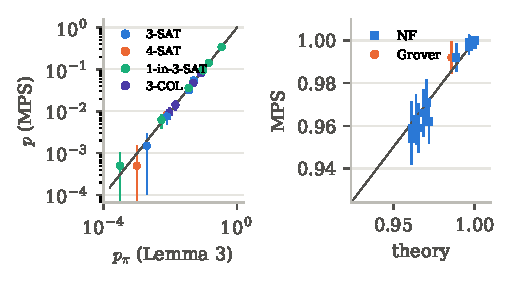
\includegraphics[width=\columnwidth]{figures/fig_mps.pdf}
\caption{\orig{ideal matrix-product-state simulation} MPS circuit simulations versus theory. Left: success probability of $A_\pi|0\rangle$ (one point per instance; error bars are $2\sigma$ shot noise). Right: success after $k^*$ amplification rounds for negation-forced (NF) and uniform (Grover) preparations; the label gives $k^*$.}
\label{fig:mps}
\end{figure}

\paragraph{E2: scaling across problem families.} \Cref{fig:scaling} and \cref{tab:scaling} report $\log_2 p$ versus $n$ for \NInstances{} instances (10 per size, 10 random orders each). Fitting $p\propto2^{-sn}$ with bootstrap confidence intervals, the effective quantum base $2^{s/2}$ drops from \GroverBaseRange{} for the uniform preparation to \NFBaseRange{} with negative conditions. The measured fraction of decisions per variable stays below the PPZ bound $1-1/k$ (\cref{tab:scaling}).

\begin{figure*}[t]\centering
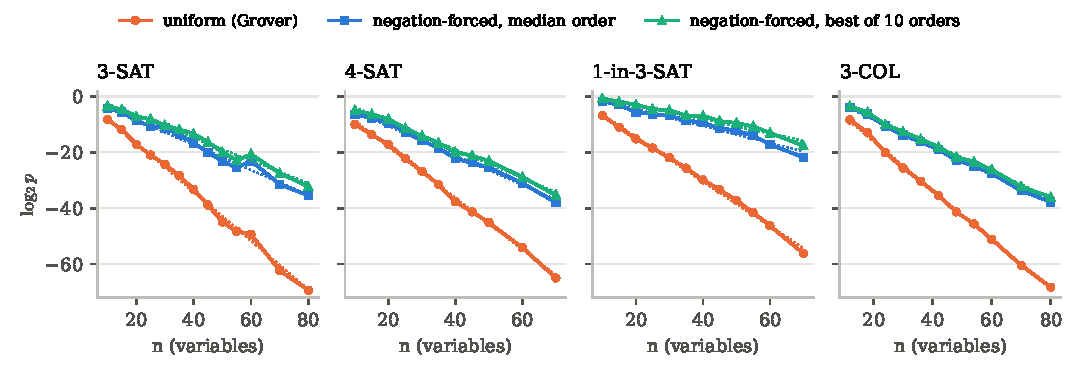
\includegraphics[width=0.95\textwidth]{figures/fig_scaling.pdf}
\caption{\orig{ideal matrix-product-state simulation} Success probability of the prepared state versus number of variables (median over 10 instances per size; dotted lines: least-squares fits). Orange: uniform superposition (Grover). Blue/green: negation-forced preparation, median and best of 10 variable orders.}
\label{fig:scaling}
\end{figure*}
\begin{table}[t]\centering\small
\caption{Fitted scaling $p\propto 2^{-sn}$ (95\% bootstrap CI) and effective quantum base $2^{s/2}$; decisions per variable $D/n$ along solutions versus the PPZ bound $1-1/k$ (for $k$-CNF).}\label{tab:scaling}
\resizebox{\columnwidth}{!}{\begin{tabular}{lrcccc}\toprule Family & inst. & Grover & NF (median) & NF (best) & $D/n$ (bound)\\\midrule
3-SAT & 130 & 1.355 & 1.169 [1.161,1.177] & 1.152 & 0.589 (0.667)\\
4-SAT & 110 & 1.375 & 1.200 [1.191,1.208] & 1.192 & 0.628 (0.750)\\
1-in-3-SAT & 120 & 1.318 & 1.110 [1.103,1.117] & 1.093 & 0.511 (--)\\
3-COL & 110 & 1.357 & 1.187 [1.182,1.192] & 1.181 & 0.630 (--)\\
\bottomrule\end{tabular}}
\end{table}

\paragraph{E3: ZX simplification.} \Cref{tab:zx} lists $T$ and two-qubit gate counts per component before and after ZX simplification, together with the equivalence checks. \ZXSummary{} For 4-SAT, PyZX extraction of the oracle (77 four-literal clauses) did not finish within one CPU-hour; ZX extraction cost is a practical limitation of the approach at this size.

\begin{table}[t]\centering\small
\caption{ZX simplification per component (mean over instances): $T$-count and two-qubit gates before $\to$ after, and the equivalence checks (statevector or MPS, see text).}\label{tab:zx}
\begin{tabular}{llrrr}\toprule Family & comp. & $T$ & 2q & $\Delta T$\\\midrule
3-SAT & $A_\pi$ & 1338$\to$536 & 1153$\to$1325 & $-60\%$\\
3-SAT & $O_F$ & 2618$\to$1130 & 2244$\to$2991 & $-57\%$\\
3-SAT & $S_0$ & 182$\to$56 & 157$\to$117 & $-69\%$\\
1-in-3-SAT & $A_\pi$ & 473$\to$205 & 448$\to$555 & $-57\%$\\
1-in-3-SAT & $O_F$ & 1036$\to$417 & 888$\to$925 & $-60\%$\\
1-in-3-SAT & $S_0$ & 182$\to$56 & 157$\to$117 & $-69\%$\\
3-COL & $A_\pi$ & 1737$\to$859 & 1506$\to$2064 & $-51\%$\\
3-COL & $O_F$ & 2688$\to$865 & 2304$\to$2166 & $-68\%$\\
3-COL & $S_0$ & 238$\to$72 & 205$\to$130 & $-70\%$\\
\bottomrule\end{tabular}
\\[2pt]\footnotesize Equivalence checks passed: 9/9 components.
\end{table}

\paragraph{E4: selecting negative conditions.} \Cref{fig:select} shows $\mathcal T(K)$ from \cref{eq:select} for $K\in\{0,1,2,3,\infty\}$, where $K=0$ is Grover's algorithm. \SelectSummary{}

\begin{figure}[t]\centering
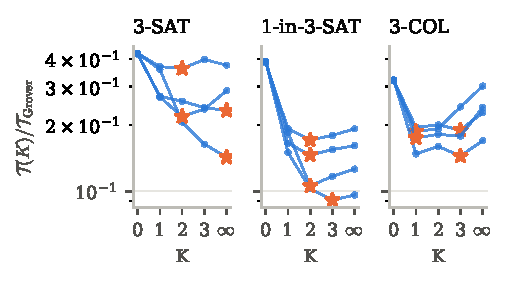
\includegraphics[width=\columnwidth]{figures/fig_select.pdf}
\caption{\orig{resource estimate (model)} Total expected $T$-count (\cref{eq:select}, after ZX) versus the number of negative conditions $K$ checked per variable and polarity, normalised by Grover ($K=0$, no ZX). Each line is one instance; stars mark $K^*$.}
\label{fig:select}
\end{figure}

\paragraph{E5: fault-tolerant resources and classical baselines.} We count logical $T$ gates of the generated circuits exactly for $n$ up to 80, combine them with the median $p$ from E2, and estimate surface-code resources~\cite{fowler2012,litinski2019} with physical error rate $10^{-3}$, threshold $10^{-2}$, logical error $p_L(d)=0.1(p/p_{\rm th})^{(d+1)/2}$, a total failure budget of $1\%$, one 15-to-1 factory~\cite{bravyi2005} and a $1\,\mu$s code cycle; ZX ratios from E3 are applied as measured averages per component (for 4-SAT, the average over the other families). \Cref{tab:resources} reports the result. \ResourceSummary{}

\begin{table*}[t]\centering\small
\caption{Fault-tolerant estimates for the median instance: expected logical $T$-count to find a solution, surface-code distance $d$, physical qubits and runtime (model in the text). Classical reps.: expected repetitions $1/p$ of the classical algorithm with the same negative conditions.}\label{tab:resources}
\begin{tabular}{lr|rrrr|rrrr|r}\toprule
 & & \multicolumn{4}{c|}{Grover (uniform)} & \multicolumn{4}{c|}{Negation-forced + ZX} & \\
Family & $n$ & $T$ & $d$ & qubits & time & $T$ & $d$ & qubits & time & classical reps.\\\midrule
3-SAT & 40 & 1.0e9 & 29 & 9.7e5 & 8.2\,h & 2.5e6 & 23 & 6.1e5 & 58.1\,s & 1.0e5\\
3-SAT & 80 & 5.3e14 & 41 & 3.8e6 & 690.3\,y & 3.1e9 & 29 & 1.9e6 & 1.0\,d & 3.9e10\\
4-SAT & 40 & 1.4e10 & 31 & 2.3e6 & 5.1\,d & 6.4e7 & 27 & 1.8e6 & 28.8\,min & 4.8e6\\
4-SAT & 70 & 3.2e14 & 41 & 7.2e6 & 420.4\,y & 2.6e10 & 33 & 4.6e6 & 10.0\,d & 2.6e11\\
1-in-3-SAT & 40 & 1.4e8 & 25 & 4.4e5 & 58.7\,min & 8.3e4 & 19 & 2.5e5 & 1.6\,s & 6.5e2\\
1-in-3-SAT & 70 & 2.3e12 & 35 & 1.5e6 & 2.6\,y & 1.0e7 & 23 & 6.4e5 & 3.8\,min & 3.3e6\\
3-COL & 30 & 6.0e7 & 25 & 4.8e5 & 25.2\,min & 9.4e5 & 21 & 3.4e5 & 19.7\,s & 1.5e4\\
3-COL & 80 & 4.2e14 & 41 & 3.4e6 & 552.7\,y & 1.0e10 & 31 & 1.9e6 & 3.6\,d & 2.4e11\\
\bottomrule\end{tabular}
\end{table*}
\paragraph{Scope and limits of these results.} The gains are relative to Grover's uniform preparation and are quadratic relative to the classical randomized algorithm that uses the same negative conditions (\Cref{tab:resources}, column ``classical reps.''). They are \emph{not} gains over industrial CDCL solvers: MiniSat solved every instance in our study with at most \MiniSatMaxConflicts{} conflicts. Random instances near the threshold are easy for CDCL at these sizes; our numerics measure exponents, not practical runtimes. Negative conditions do not reduce the number of logical qubits by themselves, since the oracle's clause register dominates; the physical-qubit savings come from fewer gates, which permits a smaller code distance. The algorithm is Las Vegas, so an error costs a repetition but never yields a wrong answer; this is error \emph{detection} at the algorithmic level, not fault tolerance. ZX optimisation and full amplification were simulated only for small instances, the large-$n$ resource estimates combine exact gate counts with ZX ratios measured at small $n$, and the surface-code model is deliberately simple. Stronger negative conditions (PPSZ-style implications via bounded-width resolution) fit the same framework, and \cref{lem:exact} still applies whenever forced values are sound.

\section{Unknown success probability: heralded weak measurement}\label{app:herald}
Theorem~\ref{thm:main} uses an exponential schedule because $p_\pi$ is unknown. On dynamic-circuit hardware an alternative is to copy the satisfaction flag weakly to a herald qubit inside every oracle call ($\mathrm{CR}_y(2\varphi_t)$, no extra queries) and measure it before the reflection; a click projects onto the solution subspace and certifies the answer before readout~\cite{mizel2009,andres2022,prabhat2026}. With the schedule $\sin^2\varphi_t=\min(1/2,5/(t+1))$ the expected cost approaches $1.01\sqrt{N/M}$ without knowing $M$, versus $\approx1.45\sqrt{N/M}$ for BBHT (\cref{tab:herald}); the 2-D model was validated against full circuit simulations. The same schedule applies verbatim to amplification over $A_\pi$ with $N/M$ replaced by $1/p_\pi$.
\begin{table}[h]\centering\small
\caption{Expected oracle queries to a verified solution, in units of $\sqrt{N/M}$ (2-D model, exact). Heralded: weak measurement of the satisfaction flag with $\sin^2\varphi_t=\min(1/2,5/(t+1))$, no knowledge of $M$.}\label{tab:herald}
\begin{tabular}{rccc}\toprule $\log_2(N/M)$ & Grover ($M$ known) & BBHT & Heralded\\\midrule
6 & 0.88 & 1.60 & 0.78\\
10 & 0.81 & 1.63 & 1.00\\
14 & 0.79 & 1.52 & 1.02\\
18 & 0.79 & 1.48 & 1.01\\
22 & 0.79 & 1.44 & 1.01\\
24 & 0.79 & 1.43 & 1.01\\
\bottomrule\end{tabular}
\end{table}

\section{Noisy intermediate-scale simulation}\label{app:noise}
For completeness, \cref{tab:noise} reports a small instance under the \texttt{FakeFez} noise model with relaxation charged to every mid-circuit measurement. At $N=16$ all methods are at the noise floor (cost $\approx8$, equal to guessing and verifying); measurement-based uncomputation (MBU: ancillas uncomputed by $X$-basis measurement and classically controlled phase fixes~\cite{gidney2018}), which needs many mid-circuit measurements, degrades sharply with latency. ``Textbook'' uses Qiskit's multi-controlled gates; ``coherent-rccx'' uses relative-phase Toffolis; ``Heralded $T$'' is the scheme of \cref{app:herald} with at most $T$ iterations. The advantages of the CNF special case discussed here therefore concern query and gate complexity in the fault-tolerant regime, not present-day hardware.
\begin{table}[h]\centering\small
\caption{Noisy simulation with the \texttt{FakeFez} (IBM Heron) noise model, binary $2\times2$ Sudoku ($N=16$, $M=2$); $L$: idle relaxation added per mid-circuit measurement. Cost: oracle queries per valid solution (random guessing: 8). Cert.: $P(\text{valid}\mid\text{herald click})$.}\label{tab:noise}
\begin{tabular}{lrrrr}\toprule Method & $L$ (ns) & $P$(valid) & cert. & cost\\\midrule
Grover textbook & 0 & 0.401 & -- & 7.5\\
Grover coherent-rccx & 0 & 0.358 & -- & 8.4\\
Grover MBU-rccx & 0 & 0.421 & -- & 7.1\\
Heralded T=2 & 0 & 0.380 & 0.67 & 7.0\\
Heralded T=4 & 0 & 0.339 & 0.57 & 11.3\\
Heralded T=6 & 0 & 0.336 & 0.49 & 14.0\\
Grover textbook & 2000 & 0.401 & -- & 7.5\\
Grover coherent-rccx & 2000 & 0.358 & -- & 8.4\\
Grover MBU-rccx & 2000 & 0.102 & -- & 29.3\\
Heralded T=2 & 2000 & 0.340 & 0.60 & 7.9\\
Heralded T=4 & 2000 & 0.308 & 0.51 & 12.5\\
Heralded T=6 & 2000 & 0.297 & 0.43 & 16.1\\
\bottomrule\end{tabular}
\end{table}


\bibliographystyle{unsrtnat}
\bibliography{refs}
\end{document}
